\documentclass{article}
\usepackage[T1]{fontenc}
\usepackage{iclr2027_conference,times}
\usepackage{amsmath,amssymb,amsthm,mathtools,bm,booktabs,graphicx,microtype,array}
\usepackage{hyperref}
\usepackage{url}
\hypersetup{hidelinks,hypertexnames=false}
\newcommand{\E}{\mathbb E}
\newcommand{\Pp}{\mathbb P}
\newcommand{\R}{\mathbb R}
\newcommand{\cD}{\mathcal D}
\newcommand{\cG}{\mathcal G}
\newcommand{\cP}{\mathcal P}
\newcommand{\GammaSet}{\mathfrak G}
\newcommand{\risk}{R^{\mathrm{pair}}_{n,\rho}}
\newcommand{\qrate}{q}
\newcommand{\TermA}{A}
\newcommand{\TermB}{B}
\newcommand{\TermM}{M}
\newcommand{\TermO}{O}
\newcommand{\TermP}{P}
\newcommand{\RateX}{X}
\newcommand{\ind}{\mathbf 1}
\newcommand{\norm}[1]{\lVert #1\rVert}
\newcommand{\abs}[1]{\lvert #1\rvert}
\newcommand{\wedgeop}{\mathbin{\wedge}}



\newtheorem{theorem}{Theorem}
\newtheorem{proposition}[theorem]{Proposition}
\newtheorem{lemma}[theorem]{Lemma}
\newtheorem{corollary}[theorem]{Corollary}
\theoremstyle{definition}
\newtheorem{definition}[theorem]{Definition}
\theoremstyle{remark}
\newtheorem{remark}[theorem]{Remark}
\newcolumntype{L}[1]{>{\raggedright\arraybackslash}p{#1}}

\title{Four-Certificate Minimax Rates over Public Class Pairs\\for Bounded Partially Linear Models}
\author{Anonymous Authors}
% \iclrfinalcopy

\begin{document}
\maketitle

\begin{abstract}
We study estimation of a bounded partially linear coefficient from two public nuisance classes with separate approximation and stochastic complexity certificates. In the strict envelope interior, the worst-public-pair expected absolute risk for \((a,s,b,t)\in[0,1]^4\) has rate
\(n^{-1/2}+(a+s^2)(b+t^2)+(s\wedge t)^2+t(a\wedge t)+s(b\wedge s)\).
Matching directional lower bounds close the gap between the Gu--Yin--Cai--Fan lower envelope and TAME's calibration upper. We also construct one rule attaining this rate without any of the four budget inputs. Double calibration removes approximation-dependent orientation, and empirical local Rademacher fixed points calibrate the stochastic radii. The general rate persists over full finite dictionary \(\ell_1\) balls and finite unions of rank-one balls. Full interval boxes instead have sharp rate \(n^{-1/2}+(a+s^2)(b+t^2)\), and full affine Hilbert balls have rate \(n^{-1/2}+ab\); both are attained without any budget input. The model requires only positive average residual variance and bounded envelopes. Results include all sample sizes and zero budgets; a uniform upper connects to saturation. The guarantees are statistical; effective optimization requires additional interfaces.
\end{abstract}

\section{Introduction}
\label{sec:intro}
A black-box nuisance class has two distinct limitations: its closest candidate can miss the truth, and learning within the class costs statistical error. How do these two limitations on each side of a partially linear model determine the best possible coefficient estimate? We characterize the risk using four upper certificates, then ask which certificates the estimating rule actually needs.

The closest results leave a precise gap. Write \(q=n^{-1/2}\), \(A=a+s^2\), \(B=b+t^2\), and \(M=(s\wedge t)^2\), where \(a,b\) are approximation budgets and \(s,t\) are stochastic budgets. Gu--Yin--Cai--Fan establish the lower envelope \(q+AB+M\) \citep{gu2026tamingbiases}. TAME's two-learner calibration construction supplies the leading upper expression
\[
 q+W,\qquad W=\min\{a(b+t)+(a+s)^2,\ b(a+s)+(b+t)^2\}
\]
\citep{gu2026optimalblackbox}. We close this gap in the bounded public-class experiment by proving matching necessity of
\[
 O=t(a\wedge t),\qquad P=s(b\wedge s).
\]
Since \(W\asymp AB+M+O+P\), these bounds establish optimality of the known two-branch rate in the stated experiment. Public budget-based orientation is already part of TAME, including its equation (3.6).

On the O ray \((a,s,b,t)=(r,0,0,r)\), the old nuisance lower is \(r^3\), while the known upper and our lower are of order \(r^2\). Taking \(r=n^{-1/8}\) makes \(q=o(r^3)\). The aggregate-error product \(xy=(a+s)(b+t)\) already equals \(r^2\) here: the improvement closes a lower-bound gap.

Convexity alone does not remove the directional terms: the same general rate holds over full finite dictionary \(\ell_1\) balls. Section~\ref{sec:adaptation} contrasts these with full interval boxes and affine Hilbert balls, whose sharp rates \(q+AB\) and \(q+ab\) are attained without budget inputs. On the ray above the three rates are \(q+r^2\), \(q+r^3\), and \(q\). These compare worst risks under different geometries with the same certificates. The distinction has a precise envelope cost: enclosing the signed dictionary \(\{0,\pm h\phi_j:j\le p\}\), with orthonormal sign functions \(\phi_j\), in a full Hilbert ball requires pointwise radius at least \(h\sqrt p\).

Section~\ref{sec:upper} supplies a second contribution: one rule attains \(q+W\) without any budget input or additional class geometry. An empirical constraint and two comparisons of the true propensity give both directions for the same rule. An independent covariate block estimates the needed complexity radii. Double calibration and empirical local complexity have established antecedents \citep{liu2023doublecalibration,bartlett2005local}; we prove the uniform expected-loss guarantee under arbitrary M1 classes. The lower also holds under every preassigned atomless covariate marginal.

\section{Experiment and four public certificates}
\label{sec:setup}
Fix a nonempty infinite standard Borel space \((\mathcal X,\mathcal A)\), shared by every law and public class below. Observe independent halves \(\cD_1,\cD_2\), each containing \(n\) iid copies of \(Z=(X,T,Y)\), with
\begin{equation}
 T=\pi_0(X)+u,\qquad Y=\beta_0T+\mu_0(X)+\varepsilon,
 \label{eq:plm}
\end{equation}
where \(\mu_0,\pi_0:\mathcal X\to\mathbb R\) are measurable, \(\E(u\mid X)=0\), \(\E(\varepsilon\mid X,T)=0\), and \(v(P):=\E u^2\in[v_-,v_+]\). Fix
\(\rho=(B_0,B_{\mathcal G},v_-,v_+,c_{\rm rad})\), with \(B_0\ge3\), \(B_{\mathcal G}>0\), \(0<v_-\le v_+\), and \(c_{\rm rad}>0\). Require
\[
 |Y|,|T|,|\mu_0(X)|,|\pi_0(X)|,|u|,|\varepsilon|\le B_0,
 \qquad \beta_0\in[-3,3].
\]
The positive average residual variance identifies the statistical coefficient: \(\E(uY)=\beta_0\E u^2\). Conditional treatment variance may vary with \(X\) and vanish on a set of positive mass.

A public instance \(\Gamma=(\cG_\mu,\cG_\pi,\mathbf g_\mu,\mathbf g_\pi)\) supplies two classes and ordered countable cores with measurable evaluations. Every full-class and represented function obeys \(|g(x)|\le B_{\mathcal G}\) for every \(x\). Our sequential M1 convention requires every full-class element to be the pointwise-everywhere limit of a sequence from its core. The common envelope transfers population approximation infima by dominated convergence and continuous finite-sample objectives by pointwise convergence.

For \(\|f\|_2=\|f\|_{L_2(P_X)}\), the approximation certificates are
\begin{equation}
 \inf_{g\in\cG_\mu}\|g-\mu_0\|_2\le a,\qquad
 \inf_{g\in\cG_\pi}\|g-\pi_0\|_2\le b.
 \label{eq:approx}
\end{equation}
Define \(\Delta\cG=\{g-g':g,g'\in\cG\}\) and the full-class localized complexity
\[
 \mathfrak R^*_{n,P_X}(r;\mathcal H)
 =\E^*_{X_{1:n},\epsilon_{1:n}}
 \sup_{h\in\mathcal H:\|h\|_2\le r}
 \left|\frac1n\sum_{i=1}^n\epsilon_i h(X_i)\right|.
\]
Here the \(\epsilon_i\) are independent Rademacher signs, independent of \(X_{1:n}\sim P_X^n\), and outer expectation is the infimum of expectations of measurable majorants. The stochastic certificates are exactly
\[
 \sup_{r\ge r_\nu,\ r>0}
 \frac{\mathfrak R^*_{n,P_X}(r;\Delta\cG_\nu)}{3r}
 \le c_{\rm rad}r_\nu,
 \qquad (\nu,r_\nu)\in\{(\mu,s),(\pi,t)\}.
\]
At zero budget this requires vanishing complexity at every positive radius. No quotient at zero is used. The countable represented difference core has measurable supremum and complexity at most the full outer complexity; equality is unnecessary and is not implied by M1.

Let \(\cP(\Gamma)=\mathcal P_{\rho,n,a,s,b,t}(\Gamma)\) be all probability laws on \(\mathcal X\times\mathbb R^2\) satisfying these model, envelope, approximation, and complexity conditions, and let \(\GammaSet_{\rho,n}(a,s,b,t)\) contain the represented pairs with \(\cP(\Gamma)\ne\varnothing\). For \((a,s,b,t)\in[0,1]^4\), define
\begin{equation}
\risk(a,s,b,t)=
\sup_{\Gamma\in\GammaSet_{\rho,n}(a,s,b,t)}
\inf_{\delta_\Gamma\ {\rm Borel}}
\sup_{P\in\cP(\Gamma)}
\E_P\abs{\delta_\Gamma(Z_{1:2n})-\beta(P)}.
\label{eq:risk}
\end{equation}
In the baseline risk \eqref{eq:risk}, the four budgets are known pre-data upper certificates, not exact errors. For each \(n\) and budget cell, the pair can change, but is fixed before Nature selects a compatible law, latent hard label, or data. The Borel rule knows \(\Gamma,\rho\) and the budgets and is fixed before the law. This order allows pair-specific rules on the one fixed ambient space. All statements include every \(n\ge1\) and every zero-budget boundary; Appendix~\ref{app:model} collects the formal measurable conventions.

\section{Sharp rate and the envelope boundary}
\label{sec:theorem}
Put
\begin{align}
 q&=n^{-1/2},& A&=a+s^2,& B&=b+t^2,\nonumber\\
 M&=(s\wedge t)^2,& O&=t(a\wedge t),& P&=s(b\wedge s),
 \label{eq:terms}
\end{align}
and write \(X=AB+M+O+P\) for the rate polynomial (distinct from the covariate).
\begin{theorem}[Three-stratum minimax law]
\label{thm:main}
Fix a nonempty infinite standard Borel measurable space
\((\mathcal X,\mathcal A)\), and fix \(B_0\ge3\), \(B_{\mathcal G}>0\),
\(0<v_-\le v_+\), and \(c_{\rm rad}>0\).  Use the sequential M1 interface above.
\begin{enumerate}
\item[\textnormal{E.}] If \(v_->B_0^2\), the experiment is empty and no minimax rate is assigned.
\item[\textnormal{I.}] If \(0<v_-<B_0^2\), there are \(0<c_\rho\le C_\rho<\infty\), depending only on fixed \(\rho\), such that, for every \(n\ge1\) and budget tuple,
\begin{equation}
c_\rho(q+X)\le\risk(a,s,b,t)\le C_\rho(q+X).
\label{eq:mainrate}
\end{equation}
One valid lower constant is one tenth the minimum of the five component constants in Appendix~\ref{app:assembly}.
\item[\textnormal{S.}] If \(v_-=B_0^2\), the upper bound holds uniformly for every legal nonempty public pair, while one explicit legal singleton pair witnesses the outer lower bound; consequently
\begin{equation}
\frac{3}{128\sqrt n}\le\risk(a,s,b,t)\le\frac1{\sqrt{2n}}.
\label{eq:saturation}
\end{equation}
\end{enumerate}
The matching constants in I are for fixed \(\rho\); in particular the lower constants need not be uniform as \(v_-\uparrow B_0^2\) or \(c_{\rm rad}\downarrow0\).
\end{theorem}

\paragraph{Average variance and the envelope boundary.}
\label{sec:boundary}
For an explicit zero-variance region, put mass \(p=v_-/B_0^2\in(0,1)\) on one of two covariate points, let \(T=\pm B_0\) equiprobably there and \(T=0\) elsewhere, and take \(\pi_0=\mu_0=\beta_0=Y=0\) and both classes \(\{0\}\). Then \(\E u^2=v_-\), while conditional variance is zero on the second point.

\begin{proposition}[Uniform one-sided envelope bound]
\label{prop:envelope-bridge}
Let \(N=2n\), let \(P_N f=N^{-1}\sum_{i=1}^N f(Z_i)\) denote the empirical average over all observations, assume \(0<v_-\le B_0^2\), and set \(\omega=1-v_-/B_0^2\). For every legal public pair and compatible law, the fixed-denominator estimator
\[
 \widehat\beta_{\rm env}=\Pi_{[-3,3]}\{P_N(TY)/B_0^2\}
 \quad\text{satisfies}\quad
 \E_P|\widehat\beta_{\rm env}-\beta(P)|\le N^{-1/2}+4\omega.
\]
The numerical constants are uniform, including in \(B_0\); this estimator uses neither \(v_+\), the four budgets, nor M1.
\end{proposition}
The envelope identity \(\E(u^2\mid X)\le B_0(B_0-|\pi_0|)\) implies \(B_0\E|\pi_0|\le B_0^2-v_-\); this controls the population bias by \(4\omega\). Appendix~\ref{app:boundary} gives the proof and the saturation lower bound. In the strict interior, comparison of the two deterministic upper guarantees gives
\[
 \risk\le\min\{C_\rho(q+X),\ q/\sqrt2+4\omega\}.
\]
This is a one-sided connection, not a matching joint transition rate. The interior lower construction uses positive slack in \(B_0-\sqrt{v_-}\).

\begin{figure}[t]
\centering
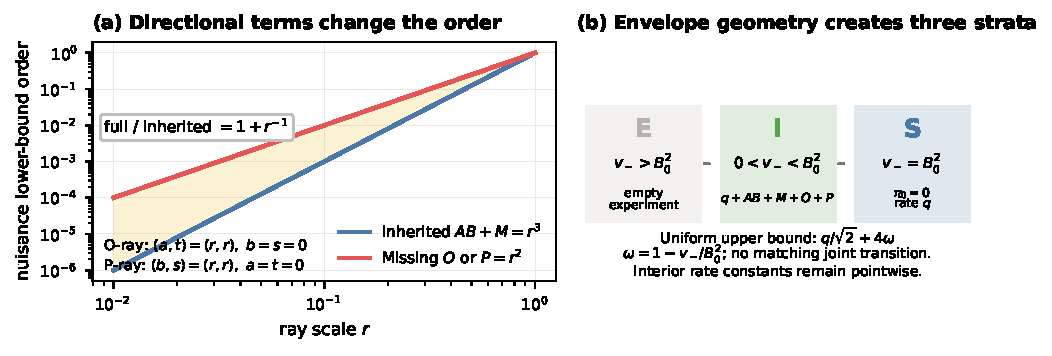
\includegraphics[width=\textwidth]{figures/theory_summary.pdf}
\caption{\textbf{Closing the directional gap and identifying the boundary.} On the O ray \((a,s,b,t)=(r,0,0,r)\), and its P mirror, the old nuisance lower is \(r^3\), while the matching rate has order \(r^2\). The ratio is \(1+r^{-1}\). Taking \(r=n^{-1/8}\) keeps \(q=o(r^3)\). The aggregate product \(xy\) already has order \(r^2\) here. The uniform upper \(q/\sqrt2+4\omega\), with \(\omega=1-v_-/B_0^2\), connects the interior to saturation; no matching joint transition rate is asserted.}
\label{fig:summary}
\end{figure}

\section{Directional lower bounds: laws, cancellation, and learning budgets}
\label{sec:lower}
Work in \(0<v_-<B_0^2\). The common treatment channel is the device that preserves exact variance while moving its mean. Set
\[
 m_\rho=\min\left\{\frac1{64},\frac{v_-}{4B_0},\frac{B_0-\sqrt{v_-}}4\right\},
 \quad\lambda_\rho=\min\left\{1,\frac{192c_{\rm rad}}{23},128B_{\mathcal G}\right\},
 \quad L=\sqrt{v_-}+2m_\rho.
\]
For \(|m|\le m_\rho\), assign treatment masses
\begin{equation}
 p_{\pm L}(m)=\frac{v_-+m^2\pm Lm}{2L^2},\qquad
 p_0(m)=1-\frac{v_-+m^2}{L^2}.
 \label{eq:treatment-channel}
\end{equation}
Indeed \(Lm_\rho\le v_-/4\), \(v_-+m_\rho^2<L^2\), and \(L+m_\rho<B_0\); thus every mass is positive and both treatment and residual envelopes hold. Direct summation gives
\[
 \E(T\mid X)=m,\qquad \E(T^2\mid X)=v_-+m^2,
 \qquad\operatorname{Var}(T\mid X)=v_-.
\]
Let \(A_Y=B_0/2\). Under each label \(\ell\), use this treatment channel at \(m=\pi_\ell(X)\) and set \(Y=A_YR\), with
\begin{equation}
 \Pr_\ell(R=r\mid X,T=\zeta)=\frac12\left[1+r\frac{\beta_\ell \zeta+\mu_\ell(X)}{A_Y}\right],
 \qquad r\in\{-1,1\}.
 \label{eq:response-channel}
\end{equation}
This specifies the entire observation law and gives the PLM conditional mean, not just a matched observable moment.

\paragraph{Two public dictionaries and their labels.}
Let \(N=2n\), and initially suppose \(n\ge16\), \(\nu^2\ge q\), with \(\nu=s\) for P and \(\nu=t\) for O, and a positive directional term. Set \(p=\lceil\exp(64N\nu^2)\rceil\). Embed a finite binary group with at least \(p\) nonzero Walsh characters into the fixed \(\mathcal X\), let \(P_X\) be uniform on its image, and extend the selected characters \(\phi_j\) by zero elsewhere. They are measurable, mean zero and orthonormal under \(P_X\). Write \(z=\sigma\phi_j(X)\).

For P, take
\[
 \eta=\frac{m_\rho(b\wedge s)}4,\quad
 \gamma=\frac{\lambda_\rho s}{256},\quad
 \Delta=\frac{2\eta\gamma}{v_-},\quad \kappa=\gamma+\Delta\eta.
\]
For O, take
\[
 \gamma=\frac{\lambda_\rho m_\rho t}4,\quad
 \eta=\frac{a\wedge t}{256},\quad
 \Delta=\frac{\gamma\eta}{v_-+\gamma^2}.
\]
Each dictionary contains the listed functions for every \(j\) and both signs, and is fixed before a label is selected:
\begin{center}
\begin{tabular}{c c c c}
\toprule
Branch & Label 0: \((\beta,\pi,\mu)\) & Label 1: \((\beta,\pi,\mu)\) & Public classes \((\cG_\mu,\cG_\pi)\)\\
\midrule
P & \((0,z\eta,z\gamma)\) & \((\Delta,-z\eta,z\kappa)\) & \((\{\pm\gamma\phi_j,\pm\kappa\phi_j\},\{0\})\)\\
O & \((0,z\gamma,z\eta)\) & \((\Delta,z\gamma,0)\) & \((\{0\},\{\pm\gamma\phi_j\})\)\\
\bottomrule
\end{tabular}
\end{center}
In P, the propensity approximation error is \(\eta\le b\) and the outcome truth is represented. In O, the outcome approximation error is at most \(\eta\le a\) and the propensity is represented. The remaining approximation distances and difference-class complexities are zero. The amplitudes give \(\kappa\le2\gamma\) and \(\Delta L+\kappa<A_Y\) in P, and \(\Delta L\le\eta/4<A_Y\) in O. Consequently the response probabilities are positive, \(|\varepsilon|\le B_0\), \(\beta\in[-3,3]\), and both public envelopes hold (Appendices~\ref{app:qp} and \ref{app:o}). Both labels have variance exactly \(v_-\), including when \(v_-=v_+\).

\paragraph{Atomwise cancellation.}
Here is why observing \((X,T,Y)\) cannot easily distinguish the coefficients. For either branch write \(d=\eta\) in P and \(d=\gamma\) in O, and define
\[
 \alpha_{\pm L}=\frac{v_-+d^2}{2L^2},\quad
 \alpha_0=1-\frac{v_-+d^2}{L^2},\quad b_\zeta=\frac{d\zeta}{2L^2}.
\]
Conditional on \(X\), the six-atom masses from \eqref{eq:treatment-channel}--\eqref{eq:response-channel} are
\begin{align*}
 \text{P: }& P_{0,z}(\zeta,r)=\tfrac12(\alpha_\zeta+zb_\zeta)(1+rz\gamma/A_Y),\\
 &P_{1,z}(\zeta,r)=\tfrac12(\alpha_\zeta-zb_\zeta)(1+r(\Delta \zeta+z\kappa)/A_Y);\\
 \text{O: }&P_{0,z}(\zeta,r)=\tfrac12(\alpha_\zeta+zb_\zeta)(1+rz\eta/A_Y),\\
 &P_{1,z}(\zeta,r)=\tfrac12(\alpha_\zeta+zb_\zeta)(1+r\Delta \zeta/A_Y).
\end{align*}
Averaging over the sign gives the same reference under the two labels precisely when
\[
 \begin{array}{ll}
 \text{P:}&\Delta\alpha_\zeta \zeta=b_\zeta(\kappa+\gamma),\quad
 \Delta(v_-+\eta^2)=\eta(\kappa+\gamma),\\
 \text{O:}&\Delta\alpha_\zeta \zeta=b_\zeta\eta,\quad
 \Delta(v_-+\gamma^2)=\gamma\eta.
 \end{array}
\]
The second identity in each row proves the first on \(\zeta=\pm L\); on \(\zeta=0\), both sides separately vanish. In P the identity follows by substituting \(\kappa=\gamma+\Delta\eta\) and \(\Delta v_-=2\eta\gamma\). Thus the common positive conditional references are
\[
 Q_P(\zeta,r)=\tfrac12(\alpha_\zeta+rb_\zeta\gamma/A_Y),\qquad
 Q_O(\zeta,r)=\tfrac12(\alpha_\zeta+rb_\zeta\eta/A_Y).
\]
This is equality of every sign-averaged atom, stronger than equality of \(\E(TY\mid X)\).

\paragraph{From cancellation to testing distance.}
Include the common marginal \(P_X\) in \(Q\). Expanding the remaining sign-linear term gives
\[
 \frac{dP_{\ell,j,\sigma}}{dQ}=1+\sigma\phi_j(X)h_\ell(\zeta,r),\qquad
 \E_Qh_\ell=0,\qquad K_\ell=\E_Qh_\ell^2.
\]
For example, in O, with \(e=\eta/A_Y\),
\[
 h_0=\frac{b_\zeta+r\alpha_\zeta e}{\alpha_\zeta+rb_\zeta e},\qquad
 h_1=\frac{b_\zeta}{\alpha_\zeta},\qquad
 K_0\le t^2/9,\quad K_1=\frac{\gamma^2}{v_-+\gamma^2}\le t^2/256.
\]
The P expansion similarly gives \(K_\ell\le s^2/196\) (Appendix~\ref{app:p-kernel}). Walsh orthogonality now yields the exact one-observation Gram entry
\[
 \E_Q\left[\frac{dP_{\ell,j,\sigma}}{dQ}
              \frac{dP_{\ell,j',\sigma'}}{dQ}\right]
 =1+\sigma\sigma'\ind\{j=j'\}K_\ell.
\]
First fix each component law, take its \(N\)-fold iid product, and only then mix the hidden coordinate and sign:
\[
 \overline P_\ell^N=\frac1{2p}\sum_{j=1}^p\sum_{\sigma=\pm1}P_{\ell,j,\sigma}^{\otimes N}.
\]
Expanding the mixture square counts \(2p\) equal-sign pairs, \(2p\) opposite-sign pairs and \(4p(p-1)\) different-coordinate pairs, giving
\begin{equation}
 \chi^2(\overline P_\ell^N,Q^{\otimes N})
 =\frac{\{(1+K_\ell)^N+(1-K_\ell)^N\}/2-1}{p}
 \le\frac{e^{NK_\ell}}p<e^{-511}.
 \label{eq:mixture-distance}
\end{equation}
The two mixtures therefore have TV distance below \(1/2\). Since each label has one common target, the midpoint testing inequality gives maximum expected absolute error at least \(\Delta/8\). Substitution yields \(\risk\gtrsim_\rho P\) and \(\risk\gtrsim_\rho O\).

\paragraph{The same dictionaries satisfy the learning certificates.}
In P the difference class has at most \(16p^2\) elements and envelope \(2\kappa\). Since \(\log(32p^2)\le258ns^2\), the finite-class Rademacher bound, applied also to every localized subset, gives
\[
 \mathfrak R_n(r;\Delta\cG_\mu)<46\kappa s
 \le\frac{23\lambda_\rho}{64}s^2,
 \qquad \frac{\mathfrak R_n(r;\Delta\cG_\mu)}{3r}
 \le\frac{23\lambda_\rho}{192}s\le c_{\rm rad}s
\]
for every \(r\ge s>0\). In O, the corresponding bound is
\(\mathfrak R_n(r;\Delta\cG_\pi)<46\gamma t\), with normalized ratio at most \(23\lambda_\rho t/384\le c_{\rm rad}t\). Thus amplitude times \(\sqrt{\log p/n}\) is of order \(\nu^2\), while the likelihood energy is also of order \(\nu^2\); the exponential dictionary makes both requirements compatible.

When \(\nu^2<q\), the corresponding interaction is at most \(q\). When \(n<16\), it is at most \(1\le4q\). These cases use the scalar lower experiment with zero nuisance classes; zero interactions need no construction. This supplies the all-\(n\) bounds without changing the active-family amplitudes.

\paragraph{Other components and assembly.}
\label{sec:assembly}
The scalar experiment perturbs only \(\beta\); the \(ab\) experiment uses two off-class truths; and the M experiment uses two represented stochastic dictionaries. Appendices~\ref{app:qp}--\ref{app:m} prove these three component bounds. The outer supremum in \eqref{eq:risk} dominates each component-specific pair. Put \(S_0=ab+M+O+P\). Expansion gives
\begin{equation}
 S_0\le X\le2S_0,
 \label{eq:budget-equivalence}
\end{equation}
since \(at^2\le O\), \(bs^2\le P\), and \(s^2t^2\le M\) on \([0,1]^4\). Taking the maximum of the five lower bounds and then their sum up to a factor five proves \(\risk\gtrsim_\rho q+X\).

Proposition~\ref{prop:same-pair-lower} additionally embeds all specified active P/O/\(ab\)/M families and the scalar family into one finite pair and one \(P_X\). Disjoint frequency bands preserve approximation distances, while the global difference-class bound pays for cross-band differences. Inactive terms use the scalar family. This simultaneous compatibility strengthens the component-wise construction; the outer lower above does not require it.

\paragraph{A preassigned covariate distribution.}
For any atomless probability \(\nu\) fixed before \(n\) and the budgets, restricting \eqref{eq:risk} to \(P_X=\nu\) preserves rate \(\asymp_\rho q+X\), with constants independent of \(\nu\), even when the learner knows it (Proposition~\ref{prop:fixed-nu-lower}). A Borel uniform coordinate transports the Walsh likelihoods. One pair still contains all specified families, but may depend on \(\nu,\rho,n\) and the budgets. This excludes arbitrary atomic marginals: a Dirac design permits order-\(q\) scalar regression.

\section{Calibration without budget inputs}
\label{sec:upper}
Write \(x=a+s\), \(y=b+t\), \(T_\mu=ay+x^2\),
\(T_\pi=bx+y^2\), and \(W=T_\mu\wedge T_\pi\).
TAME supplies the calibration branches and budget-based orientation
\citep{gu2026optimalblackbox}; Appendix~\ref{app:upper} supplies the complete
known-budget implementation and expected-loss proof.
\begin{proposition}[Known-budget class-pair upper]
\label{prop:upper}
That rule satisfies
\(\sup_{P\in\cP(\Gamma)}\E_P|\widehat\beta_\Gamma-\beta(P)|
\le C_\rho(q+X)\) for every fixed legal pair, uniformly in \(n,a,s,b,t\).
\end{proposition}
The selector and rate algebra are
\begin{equation}
 T_{\rm selected}\le2W\le48X,\qquad X/5\le W\le24X.
 \label{eq:selector-algebra}
\end{equation}
We remove all four inputs by combining double calibration
\citep[Section 4.1]{liu2023doublecalibration} and classical empirical local
Rademacher fixed points \citep{bartlett2005local}, with a uniform guarantee
under the original interface.

\begin{theorem}[Adaptation to all four budgets]
\label{thm:approximation-main}
For every fixed \((\Gamma,\rho,n)\), one Borel rule
\(\widehat\beta_{\rm ad}\), using none of \(a,s,b,t\), satisfies
\[
 \forall(a,s,b,t)\in[0,1]^4,\quad
 \sup_{P\in\mathcal P_{\rho,n,a,s,b,t}(\Gamma)}
 \E_P|\widehat\beta_{\rm ad}-\beta(P)|\le C_\rho(q+W)
\]
whenever the compatible-law set is nonempty. The constant depends
only on \(\rho\); no additional class geometry is imposed.
\end{theorem}

\paragraph{Estimating the two complexity radii.}
Above a fixed sample threshold, split the \(2n\) observations into three
blocks of size \(m=\lfloor2n/3\rfloor\), discarding at most two.
Use only covariates from block \(\mathcal C\) for calibration.
Let \(Q_{\mathcal C}\) be its empirical average,
\(L_0=1\vee2B_{\mathcal G}\),
\(\mathcal F_\nu=\Delta\cG_\nu^{\rm rep}/L_0\), and compute
\[
 \widehat\psi_\nu(r)=20\E_\epsilon\sup_{f\in\mathcal F_\nu}
 \left(1\wedge\sqrt{\frac{2r}{Q_{\mathcal C}f^2}}\right)
 |Q_{\mathcal C}(\epsilon f)|+\frac{186\log(em)}m .
\]
Zero empirical norms contribute zero. This star-hull complexity with a
positive floor has a unique positive fixed point \(\widehat r_\nu\).
Set \(\widehat s=1\wedge C_0L_0\sqrt{\widehat r_\mu}\) and
\(\widehat t=1\wedge C_0L_0\sqrt{\widehat r_\pi}\),
where \(C_0=1\vee(60c_{\rm rad})^{-1}\).
Appendix~\ref{app:stochastic-adaptation} proves that, except with probability
\(8(em)^{-6}\), these are valid size-\(m\) full-class certificates with
\(c_{\rm rad}\) replaced by \(2c_{\rm rad}\), and
\(\widehat s\le C_\rho(s+h)\), \(\widehat t\le C_\rho(t+h)\),
where \(h^2=\log(em)/m\). The public classes are unchanged. Using a first crossing without the
star hull can fail when smaller localized balls contain only zero.

\paragraph{One calibrated rule for both directions.}
On the remaining main and fitting blocks, let \(P_1,P_2\) be their
empirical averages, \(\|w\|_m^2=P_1w^2\), and \(\tau=m^{-12}\).
All constants below are fixed using
\(\rho'=(B_0,B_{\mathcal G},v_-,v_+,2c_{\rm rad})\).
Fit \(\widehat\pi\) and jointly \((\widehat\beta_0,\widehat\mu)\)
by represented least squares on the fitting block. Its internal
train/validation split also supplies a fixed-anchor scalar pilot
\(\bar\beta\). Set
\(\kappa_\mu=K(\widehat s^2+h^2)\),
\(\kappa_\pi=K(\widehat t^2+h^2)\), and
\(A_{\widehat t}=K_A(\widehat t^2+h^2)\).
First approximately minimize \(\|w-\widehat\mu_X\|_m^2\) over
\(w\in\mathbb Q^m\), subject to
\[
 \sup_{f\in\Delta\cG_\pi^{\rm rep}}
 \{|P_2[(Y-\bar\beta T)f]-P_1(wf)|-P_1f^2\}<\kappa_\pi,
 \qquad \|w\|_m<M_{\rho'}.
\]
Call the result \(\widehat\eta\), put \(d=\widehat\eta-\widehat\mu_X\),
and define
\(H_\nu(r)=\sup_{f\in\Delta\cG_\nu^{\rm rep}}
\{|P_1(rf)|-P_1f^2\}\).
Next minimize \(\|z\|_m^2\) over
\(g\in\cG_\pi^{\rm rep}\), \(z\in\mathbb Q^m\).
Writing \(\widetilde\pi=g_X+z\), \(r=T_X-\widetilde\pi\) and
\(D=P_1(Tr)\), impose
\[
 \begin{gathered}
 P_1(g-\widehat\pi)^2<A_{\widehat t},\quad D>v_-/2,\quad
 \|r\|_m,\|\widetilde\pi\|_m<R_{\rho'},\quad
 H_\nu(r)<\kappa_\nu\quad(\nu=\mu,\pi),\\
 |P_1(rw)|<8B_0h\|w\|_m+\tau
 \quad\text{for }w\in\{d,\widetilde\pi,z\}.
 \end{gathered}
\]
The output is
\(\widehat\beta_{\rm ad}
=\Pi_{[-3,3]}\{P_1[r(Y-\widehat\eta)]/D\}\).
Take the first feasible candidate within \(\tau\) of each infimum;
infeasibility or small \(n\) gives zero. These choices and the fixed
points are jointly Borel, without a finite-query optimization guarantee.

\paragraph{Why the guarantee adapts.}
Given a good calibration block, the remaining samples retain their iid
law and the radii are valid fixed inputs. The pilot error \(c=\beta_0-\bar\beta\)
has second moment at most
\(C_\rho\min\{a^2+\widehat s^2+h^2,b^2+\widehat t^2+h^2\}\).
The first edit uses fitting data and main covariates, with comparison
\(\eta_0=\mu_0+c\pi_0\). The second also uses main treatments;
main outcomes enter only the final ratio. Treatment noise is centered
against directions fixed by fitting data and main covariates;
outcome noise after additionally conditioning on main treatments.

On a further event of probability \(1-O_\rho(m^{-4})\),
\(g=\widehat\pi,z=\pi_0-\widehat\pi\) represents the true propensity
with zero class cost and strict feasibility margins.
When \(b\le\widehat t+h\), a fixed close core function \(g_0\) supplies
the second comparison \(g=g_0,z=\pi_0-g_0\).
Rational approximation transfers these comparisons to the same
minimum of \(\|z\|_m^2\). Outcome calibration squares the represented
fit error; propensity calibration exploits the smaller free residual.
For larger \(b\), the same rule's product bound applies.
The split partitions only the proof.
Appendix~\ref{app:approximation-adaptation} gives the resulting conditional
risk bound
\[
 C_\rho\left[m^{-1/2}+
 \min\{a(b+\widehat t)+a^2+\widehat s^2,\
        b(a+\widehat s)+(b+\widehat t)^2\}\right].
\]
The radius bounds, \(ah\le(a^2+h^2)/2\),
\(bh\le(b^2+h^2)/2\), and \(h^2\le4q\) turn this into \(C_\rho(q+W)\).
Clipping pays for calibration failure. Appendix~\ref{app:stochastic-adaptation}
proves the transfers and zero-budget cases; only \(\Gamma,\rho,n\) are inputs.

\section{Class geometry and budget adaptation}
\label{sec:adaptation}
Restricting the outer supremum in \eqref{eq:risk} to the displayed geometries gives different minimax rates. Write \(\mathcal R_{\rm box}\) and \(\mathcal R_{\rm Hilb}\) for full box and full affine Hilbert pairs. All these rates admit rules without budget inputs; the distinction below is the available class geometry.

\paragraph{Full interval boxes.}
For each \(\nu\in\{\mu,\pi\}\), allow its own countable Borel partition and
\[
 \cG_\nu=\left\{c_\nu+\sum_j\theta_j\mathbf1_{C_{\nu j}}:
 |\theta_j|\le h_{\nu j}\right\},\qquad
 |c_\nu(x)|+h_{\nu j}\le B_{\mathcal G}\quad(x\in C_{\nu j}).
\]
All coordinate choices are included; the public centers may vary within cells. Recover \(c_\nu,h_\nu\) as the midpoint and half-range of its core evaluations. Group equal centered core profiles, which recover occupied positive-width cells. Set \(N=2n\), \(\alpha=\min\{1/8,v_-/(8B_0^2)\}\), and \(m=\lfloor\alpha N\rfloor\). On each side, trim the \(m\) largest-width singleton rows, or all if fewer exist, resolving ties by sample index. Let \(\mathsf A_\nu\) center repeated groups, vanish on trimmed rows, and retain other singletons. Define
\[
 \begin{gathered}
 \mathsf B=\mathsf A_\pi\mathsf A_\mu,\quad
 D=(T-c_\pi)'\mathsf BT/N,\quad U=(T-c_\pi)'\mathsf B(Y-c_\mu)/N,\\
 S=T'\mathsf A_\mu T/N,\qquad V=T'\mathsf A_\mu(Y-c_\mu)/N.
 \end{gathered}
\]
\begin{equation}
 \widehat\beta_{\rm box}=
 \begin{cases}
 \Pi_{[-3,3]}(U/D),&D\ge v_-/32,\\
 \Pi_{[-3,3]}\{V/(S\vee(v_-/4))\},&D<v_-/32.
 \end{cases}
 \label{eq:histogram-estimator}
\end{equation}
\begin{proposition}[Sharp box rate without budget inputs]
\label{prop:histogram-adaptation}
For every fixed represented box pair and \(n\ge1\), the same Borel rule \eqref{eq:histogram-estimator} satisfies
\[
 \E_P|\widehat\beta_{\rm box}-\beta(P)|\le C_\rho\{q+(a+s^2)(b+t^2)\}
\]
simultaneously for all four certificate tuples and compatible laws. In the strict interior,
\(\mathcal R_{\rm box}\asymp_\rho q+AB\).
\end{proposition}
The key is selective retention of singletons. For either side put
\(H=N^{-1}\sum_jh_j\mathbf1_{\{N_j=1\}}\). The complexity certificate and a one-observation replacement bound give
\[
 \E H\le C_\rho r^2,\qquad
 \E H^2\le C_\rho r^4+2B_{\mathcal G}^2/N.
\]
After trimming, every retained width is at most \(H/\alpha\); hence each public residual has expected squared norm \(O_\rho(r^4+N^{-1})\). Writing
\(F_\nu=\|\mathsf A_\nu(\nu_0-c_\nu)_X\|_N\), both the primary bias and the event-weighted fallback bias are controlled by
\(\E(F_\mu F_\pi)\le C_\rho\{AB+q\}\).
At most \(2\alpha N\) diagonal entries of \(\mathsf B\) lose the \(1/4\) lower bound. A small cross denominator forces \(F_\pi\) above a fixed constant outside an \(O_\rho(n^{-1})\) event.

For the matching lower, full boxes of widths proportional to \(s^2,t^2\) have global difference complexity bounded by twice their width, regardless of host size. Rescaling the two cancellation channels above yields gaps \(ab,at^2,bs^2,s^2t^2\); an exponential Walsh host hides their mixtures. Appendix~\ref{app:budget-adaptation} supplies both complete proofs. This lower bound concerns the restricted outer supremum, not every fixed box.

\paragraph{Full affine Hilbert balls.}
Suppose \(\cG_\nu=c_\nu+R_\nu B_{\mathcal H_\nu}\) is an entire reproducing-kernel Hilbert ball obeying the same envelope and M1 interface. The two kernels may differ and have overlapping features or infinite rank. Polarization of centered-core evaluation suprema recovers the normalized kernels \(\ell_\nu=R_\nu^2k_\nu\) without extra inputs. Let \(M_c\) project off the two sampled center vectors and put
\[
 H=M_c[\ell_\mu(X_i,X_j)+\ell_\pi(X_i,X_j)]_{i,j}M_c/N,\quad
 \lambda=\frac{16B_{\mathcal G}^2B_0^2}{Nv_-},\quad
 A_c=M_c(I+H/\lambda)^{-1}M_c.
\]
For \(N\ge16B_0^2/v_-\), use
\(\widehat\beta_{\rm Hilb}=\Pi_{[-3,3]}\{T'A_cY/(T'A_cT\vee Nv_-/4)\}\);
otherwise output zero.
\begin{proposition}[Hilbert-ball comparison]
\label{prop:hilbert-main}
The same fixed-\((\Gamma,\rho,n)\) rule satisfies
\(\E_P|\widehat\beta_{\rm Hilb}-\beta(P)|\le C_\rho(q+ab)\)
for every certificate tuple and compatible law. In the strict interior,
\(\mathcal R_{\rm Hilb}\asymp_\rho q+ab\), allowing zero-radius balls.
\end{proposition}
In this large-sample branch, \(\operatorname{tr}(I-A_c)\le Nv_-/(4B_0^2)\) and
\(\sup_{g\in\cG_\mu\cup\cG_\pi}\|A_cg_X\|_N\le\sqrt\lambda/2\).
These preserve average variance and leave \(ab+O_\rho(q)\) bias.
Appendix~\ref{app:hilbert-adaptation} proves the result; its outer lower already holds for the zero pair.
This is a bounded misspecification guarantee for classical penalized partialling-out
\citep{heckman1986spline,zhao2016partially}, not a new estimator family.
Finite versions require evaluable centers together with partition labels and widths, or kernel evaluations, respectively; M1 alone gives Borel existence.

\begin{proposition}[Convex hulls and finite unions]
\label{prop:convex-geometry}
For full dictionary \(\ell_1\) balls
\(\{\sum_{j=1}^k\theta_jd_j:\sum_j|\theta_j|\le1\}\), and for segment
unions \(\bigcup_{j=1}^k\{\tau d_j:|\tau|\le1\}\), both restricted
outer risks are \(\asymp_\rho q+X\) in the strict interior.
Zero classes are allowed and \(k\) may grow with \(n\) and the budgets.
Each segment is a full RKHS ball of rank at most one.
\end{proposition}
Enlarging the same-pair dictionaries this way preserves global difference
complexity \citep[Theorem 12(2)]{bartlett2002rademacher}; off-band truths
remain orthogonal to the enlarged span. Every certificate and testing
lower therefore survives. Localized complexities need not be equal.
Moreover, enclosing \(\{0,\pm h\phi_j:j\le p\}\), for orthonormal sign
functions \(\phi_j\), in a full affine Hilbert ball requires pointwise radius at least
\(h\sqrt p\), sharply (Appendix~\ref{app:convex-geometry}).
Convexity or a finite union alone thus does not give the Hilbert rate.

\section{What the rate says about nuisance imbalance}
\label{sec:interpretation}
\label{sec:mechanisms}
\begin{corollary}[Optimal calibration and certificate allocation]
\label{cor:allocation}
Fix \(\rho\) in the interior stratum. Then \(\risk\asymp_\rho q+W\). On \(0<x\le y\),
\[
 \frac{\risk}{xy}\asymp_\rho\frac{q}{xy}+\frac ax+\frac xy.
\]
Along any such sequence with \(q=o(xy)\), \(\risk=o(xy)\) if and only if \(a=o(x)\) and \(x=o(y)\). For \(0<y<x\), interchange \((a,x)\) and \((b,y)\).
For \(0<x\le y\le1\), put
\(\mathcal A(x,y)=\{(a,s,b,t)\in[0,1]^4:a+s=x,\ b+t=y\}\). Then
\[
 \inf_{\mathcal A(x,y)}\risk\asymp_\rho q+x^2,
 \qquad \sup_{\mathcal A(x,y)}\risk\asymp_\rho q+xy.
\]
\end{corollary}
Divide the selected-branch rate by \(xy\). For allocation,
\(x^2/4\le X\le4xy\), with endpoints \((0,x,y,0)\) and \((x,0,y,0)\);
see Appendix~\ref{app:allocation-proof}. TAME's sufficient imbalance
conditions are therefore necessary in this experiment. The benchmark
\(xy\) describes a guarantee, not a lower bound for a particular DML algorithm.

\section{Related work, limitations, and conclusion}
\label{sec:related}
Gu--Yin--Cai--Fan Theorem A.1 gives \(q+AB+M\) in a fixed-covariate, constant-variance field \citep{gu2026tamingbiases}. TAME Corollary 3.2, equations (3.6)--(3.7), gives the orientation, tuning, and leading upper \(q+W\); Condition 2.1(b) already uses average residual variance \citep{gu2026optimalblackbox}. SADE Theorem 2.1 and Remark 2.1 give budget-free single-outcome-class adaptation \citep{gu2026tamingbiases}; our results concern the sharp two-class risk and simultaneous adaptation to its four certificates.

Jin--Mackey--Syrgkanis Theorem 3.1 gives squared-radius and mixed-product obstructions around fixed estimates of \((\E[T\mid X],\E[Y\mid X])\) in binary-treatment PLMs \citep{jin2025hardnormal}. Because \(\E[Y\mid X]=\mu_0+\beta_0\pi_0\) changes with the target, those anchored radii are not our four certificates. The obstruction concepts are inherited; our cancellation constructions preserve the four certificates and a common variance. Related fields include anchored product bounds \citep{jin2026sharpstructureagnostic}, calibrated inference \citep{vanderlaan2025calibrateddml}, and fixed-pilot asymptotic risk \citep{liu2026dmlinadmissibility}.

\paragraph{Limitations.}
The general adaptive rule knows the represented pair and \(\rho\); it is Borel but need not have a finite-query implementation. Lower dictionaries may be exponential. Faster box and Hilbert rates require their full-class geometry and envelopes. Selection across different public pairs and effective optimization remain open. Constants depend on fixed \(\rho\); the joint envelope transition is unresolved. No causal, inference, or empirical performance guarantee is supplied.

\paragraph{Conclusion.}
Matching O/P bounds close the known calibration rate. Double calibration and empirical complexity estimation attain it without any budget input. The rate persists for dictionary \(\ell_1\) balls, while full boxes and Hilbert balls admit faster rates. The sharp enclosure cost prevents a same-envelope transfer of the dictionary lower to Hilbert balls.

\clearpage
\subsection*{Reproducibility statement}
This paper is theoretical.  The appendices give all proofs, reductions,
constants, and audits.  Figure~\ref{fig:summary} is generated analytically by
\nolinkurl{figures/+generate_theory_summary.py}; from the source-tree root, run
% Portable command: <PYTHON_EXECUTABLE> figures/+generate_theory_summary.py
\texttt{<PYTHON\_EXECUTABLE>}\ \texttt{figures/+generate\_theory\_summary.py}.
It contains no empirical or simulated performance evidence.

\subsection*{AI use statement}
Generative AI assisted discovery, literature work, proof drafting and auditing,
symbolic checks, figures, and editing.  The authors reviewed all AI-assisted work
and take responsibility for the final content, including text, mathematical
claims, proofs, and artifacts produced with AI assistance.  No
AI-generated empirical evidence is reported.

\bibliography{references}
\bibliographystyle{iclr2027_conference}

\appendix
\section{Full model, measurable access, and minimax quantifiers}
\label{app:model}

\subsection{Measurable experiment and statistical target}

Fix once and for all a nonempty infinite standard Borel measurable space
\((\mathcal X,\mathcal A)\).  This fixed nonempty infinite standard Borel measurable space is shared by every public pair and law below.  Equip
\[
 \mathcal Z=\mathcal X\times\mathbb R\times\mathbb R
\]
with the product sigma-field
\(\mathcal A\otimes\mathcal B(\mathbb R)\otimes
\mathcal B(\mathbb R)\).  The coordinates
\(X:\mathcal Z\to\mathcal X\), \(T,Y:\mathcal Z\to\mathbb R\) are
measurable, and all conditional expectations are ordinary versions on this
probability space.  Public represented functions are jointly supplied with
measurable evaluation maps \(x\mapsto g_j(x)\).  This standard-Borel
condition is part of the theorem field before \(n\), the budget tuple, the
public pair, and the compatible law are chosen.  It excludes pathological
nonstandard measurable spaces and finite ambient spaces from the matching
I-stratum theorem, while including countably infinite and uncountable
standard Borel spaces used in ordinary ML models.

For a fixed regularity tuple
\[
 \rho=(B_0,B_{\mathcal G},v_-,v_+,c_{\rm rad}),\qquad
 B_0\ge3,\quad B_{\mathcal G}>0,\quad
 0<v_-\le v_+,\quad c_{\rm rad}>0,
\]
a law in \(\cP(\Gamma)\) satisfies \eqref{eq:plm},
\(\E(u\mid X)=0\), \(\E(\varepsilon\mid X,T)=0\), and
\(v:=\E u^2\in[v_-,v_+]\).  The conditional variance
\(\operatorname{Var}(T\mid X)=\E(u^2\mid X)\) may vary with \(X\)
and may vanish on subsets of the covariate space.  It also satisfies
\[
 |Y|,|T|,|\beta_0|,|\mu_0(X)|,|\pi_0(X)|,|u|,|\varepsilon|
 \le B_0,\qquad \beta_0\in[-3,3].
\]
The target is the statistical coefficient \(\beta_0\) in this conditional
mean model.  Causal interpretation would require additional assumptions and
is not asserted.

Every admissible public pair also satisfies the fixed pointwise candidate
envelope
\[
 \sup_{g\in\cG_\mu\cup\cG_\pi}|g(x)|\le B_{\mathcal G}
 \qquad\text{for every }x\in\mathcal X.
 \tag{A.0}
\]
Every function in the supplied countable representations obeys the same
bound.  Thus each public difference class has envelope \(2B_{\mathcal G}\).
This condition is part of the fixed theorem field before the outer public-pair
supremum; it is not inferred from approximation or localized complexity.

\subsection{Positive-radius public complexity and M1 access}

For a public class \(\cG\), let
\(\Delta\cG=\{g-g':g,g'\in\cG\}\).  For any class \(\mathcal H\) and
\(r\ge0\), put
\[
 Z_{\mathcal H}(r):=
   \sup_{\substack{h\in\mathcal H\\ \norm h_{L_2(P_X)}\le r}}
   \abs{\frac1n\sum_{i=1}^n\epsilon_i h(X_i)},\qquad
 \mathfrak R^{*}_{n,P_X}(r;\mathcal H)
 :=\E^{*}_{X_{1:n},\epsilon_{1:n}} Z_{\mathcal H}(r).
\]
Here \(X_{1:n}\sim P_X^n\), the \(\epsilon_i\)'s are independent Rademacher
signs independent of the sample, and the outer expectation \(\E^*Z\) is the
infimum of \(\E U\) over all measurable majorants \(U\ge Z\).  When
\(Z_{\mathcal H}(r)\) is measurable, outer and ordinary expectation agree.
If \(\cG^{\rm rep}=\{g_j:j\in\mathbb N\}\), its countable represented difference core is
\(\Delta\cG^{\rm rep}=\{g_j-g_k:j,k\in\mathbb N\}\).  Its supremum is an ordinary measurable random variable, and we write its ordinary-expectation
complexity as \(\mathfrak R_{n,P_X}(r;\Delta\cG^{\rm rep})\).  Pointwise
set inclusion and monotonicity of outer expectation give
\[
 \mathfrak R_{n,P_X}(r;\Delta\cG^{\rm rep})
 \le \mathfrak R^{*}_{n,P_X}(r;\Delta\cG).
\]
Equality is not required, and sequential M1 alone does not provide it.  At
\(r=0\) the unquotiented quantities above remain defined.  No
star-shapedness or scaling closure is assumed or used.  The stochastic
constraints are exactly
\begin{align}
 \sup_{r\ge s,\ r>0}
 \frac{\mathfrak R^{*}_{n,P_X}(r;\Delta\cG_\mu)}{3r}
 &\le c_{\rm rad}s,\nonumber\\
 \sup_{r\ge t,\ r>0}
 \frac{\mathfrak R^{*}_{n,P_X}(r;\Delta\cG_\pi)}{3r}
 &\le c_{\rm rad}t.
 \tag{A.1}
\end{align}
No positive-radius quotient at \(r=0\) is defined or used.  When a declared
stochastic budget is zero, (A.1) directly forces the corresponding full-class
outer complexity, and hence every represented-core complexity, to vanish at
each positive radius.  Later upper-proof calls therefore use core base radius
zero directly; they never evaluate a radius-zero quotient.

M1 means that the learner receives the represented public instance
\[
 \Gamma=(\cG_\mu,\cG_\pi,\mathbf g_\mu,\mathbf g_\pi),\qquad
 \mathbf g_\nu=(g_{\nu,j})_{j\in\mathbb N},\quad \nu\in\{\mu,\pi\},
\]
where \(\mathbf g_\nu\) is an ordered countable representation of
\(\cG_\nu\).  It also receives the fixed
tuple including \(B_{\mathcal G}\), and the four declared budgets before
observing data.  The representation has measurable evaluations, obeys the
same envelope, and has the following sequential property: for every
full-class element \(g\in\cG\), there is a sequence \(g_{j_k}\) from the
representation that converges pointwise everywhere to \(g\) on \(\mathcal X\).
The common envelope and dominated convergence make the represented and
full-class population \(L_2(P_X)\) approximation infima equal; finite-sample
continuity gives the corresponding empirical fit and calibration transfers.
Empirical approximate minimizers select the first represented index within
\(n^{-12}\) of a countable infimum.
Scalar coefficients use \(\mathbb Q\cap[-3,3]\); finite-dimensional convex
objectives use objective-dense rational parameterizations.  Countable
infima, first qualifying indices, finite arithmetic, and clipping are
measurable, so every fitted rule is Borel.  M1 does not supply nuisance truths,
population best approximants, realized errors, a hard label, or an
optimization oracle.

\begin{definition}[Indexed compatible-law class]
\label{def:indexed-compatible-laws}
Fix \(\rho,n,a,s,b,t\), and let
\(\Gamma=(\cG_\mu,\cG_\pi,\mathbf g_\mu,\mathbf g_\pi)\) be a represented
public instance obeying the envelope and measurable sequential-M1 interface
above.  We call \((\cG_\mu,\cG_\pi)\) its class-pair projection.  The indexed compatible-law class
\(\mathcal P_{\rho,n,a,s,b,t}(\Gamma)\) is the set of probability laws
\(P\) on \(\mathcal Z\) for which there are
\(\beta_0\in[-3,3]\),
\(\mathcal A/\mathcal B(\mathbb R)\text{-measurable functions }\mu_0,\pi_0:\mathcal X\to\mathbb R\),
and residuals
\[
 u=T-\pi_0(X),\qquad
 \varepsilon=Y-\beta_0T-\mu_0(X),
\]
such that the PLM representation \eqref{eq:plm}, the conditional-centering
conditions
\(\E(u\mid X)=0\) and \(\E(\varepsilon\mid X,T)=0\) hold
\(P\)-almost surely, and the average residual-variance condition
\(v:=\E_P u^2\in[v_-,v_+]\) holds.  The shared law and target envelopes are
\[
 |Y|,|T|,|\beta_0|,|\mu_0(X)|,|\pi_0(X)|,|u|,|\varepsilon|
 \le B_0,
\]
and the public classes and their representations retain the pointwise
candidate envelope (A.0), measurable evaluation maps, and the
pointwise-everywhere sequential-M1 approximation property.  Under this
law's covariate marginal \(P_X\), the approximation-budget conditions are
\[
 \inf_{g\in\cG_\mu}\norm{g-\mu_0}_2\le a,
 \qquad
 \inf_{g\in\cG_\pi}\norm{g-\pi_0}_2\le b,
\]
and the localized-complexity conditions are
\[
 \sup_{r\ge s,\ r>0}
 \frac{\mathfrak R^{*}_{n,P_X}(r;\Delta\cG_\mu)}{3r}
 \le c_{\rm rad}s,
 \qquad
 \sup_{r\ge t,\ r>0}
 \frac{\mathfrak R^{*}_{n,P_X}(r;\Delta\cG_\pi)}{3r}
 \le c_{\rm rad}t.
\]
The target \(\beta(P)\) is uniquely identified: if two such conditional-mean
PLM representations describe the same law, their conditional-mean difference
is \(\gamma T+f(X)=0\) almost surely.  Conditional centering identifies
\(\pi_0(X)=\E(T\mid X)\), hence the same residual \(u\), in both
representations.  Multiplying the difference by \(u\) and taking
expectations gives \(0=\gamma\E u^2\), since
\(\E\{f(X)u\}=\E\{\pi_0(X)u\}=0\).  Because
\(\E u^2\ge v_->0\), \(\gamma=0\), so the two coefficients agree.
Apart from recording this consequence, this
definition merely collects the model, envelope, approximation,
positive-radius complexity, and public measurable-access predicates already
stated above; it changes none of them.  In the main text and the rest of the
appendices we suppress the fixed indices \(\rho,n,a,s,b,t\) and write
\(\cP(\Gamma)\).
\end{definition}

\subsection{Q1 order and allowed sample-size dependence}

For each integer \(n\ge1\) and budget tuple, define
\(\GammaSet_{\rho,n}(a,s,b,t)\) as the collection of represented public
pairs on this same fixed ambient space satisfying the candidate-envelope and
measurable sequential-M1 fields above and having
\(\mathcal P_{\rho,n,a,s,b,t}(\Gamma)\ne\varnothing\).  The ambient space is not a coordinate
of \(\Gamma\) and is not varied by the outer supremum.
Q1 is the order printed in \eqref{eq:risk}:
\[
 \sup_{\Gamma\in\GammaSet_{\rho,n}(a,s,b,t)}
 \inf_{\delta_\Gamma\ {\rm Borel}}
 \sup_{P\in\cP(\Gamma)}
 \E_P|\delta_\Gamma(Z_{1:2n})-\beta(P)|.
\]
The public pair and a lower hard family may depend on \(n\) and the declared
budgets, but they are fixed before the data and before any latent label,
coordinate, or sign is drawn.  Dependence on realized data is prohibited.
No single class pair is required to serve all sample sizes or all budget
cells.  For each fixed \(\Gamma\), the decision rule may depend on
\(\Gamma,\rho,a,s,b,t\) but not on \(P\), proof-only comparators, or
realized errors.  Hence the outer public-pair supremum is taken only after the
fixed-pair rule and its uniform law bound are established.

The total sample size is \(N=2n\), while \(q=n^{-1/2}\); replacing \(q\) by
\(N^{-1/2}\) changes only a fixed factor.  Risk is expected absolute error.
All interior constants may depend on fixed \(\rho\), including
\(B_{\mathcal G}\), but not on
\(n,a,s,b,t,\Gamma,P\).  At \(c_{\rm rad}=0\), (A.1) collapses every legal
difference class in \(L_2(P_X)\), and the positive-budget nuisance lower is
false.  Thus the theorem is pointwise for \(c_{\rm rad}>0\), with constants
that may degenerate as \(c_{\rm rad}\downarrow0\); it is not uniform at that
boundary.

\section{Complete proof of the global upper bound}
\label{app:upper}

This appendix defines the estimator and proves every stochastic and
deterministic step used in Proposition~\ref{prop:upper}.  No result from an
internal proof package is an assumption below.  Throughout, \(P_j\) denotes
the empirical average on half \(\cD_j\), \(j=1,2\).  Every unnamed proof
constant depends only on the fixed tuple \(\rho\).  Throughout, put
\(v:=\E u^2\in[v_-,v_+]\); no constant or positive pointwise
conditional treatment variance is assumed.  Put
\[
 \norm{f}_{1,n}:=(P_1f^2)^{1/2},\qquad
 \norm{f}_{2,n}:=(P_2f^2)^{1/2}.
\]
These half-indexed symbols are used for fitted functions of \(X\).  A vector
norm whose sample half is already fixed by its definition retains the shorter
notation \(\norm\cdot_n\).
Put
\[
 C_f=1+\frac{B_0}{\sqrt{v_-}},\qquad
 C_J=1+3C_f+\frac{B_0}{c_{\rm rad}\sqrt{v_-}}.
\]
Let \(K_{1,\star}\) be the maximum of the primitive radius constants in
Lemma~\ref{lem:localized-process} for the seven calls listed explicitly in
the event ledger below.  They use only the two public difference cores and
the joint class, on a specified sample half, with a specified multiplier or
square process, before any fitted index is substituted.  Fix
\[
 C_{\rm rad}:=1+K_{1,\star}(1+C_J),\qquad
 K_\lambda:=1,\qquad K_d:=8.
\]
Here the model parameter \(c_{\rm rad}>0\) is distinct from the
proof/estimator inflation constant \(C_{\rm rad}\).  Also put
\[
 B_\pi=B_0+B_{\mathcal G},\qquad
 B_{\rm all}=B_0+4B_{\mathcal G},\qquad
 \vartheta_\rho=\frac{B_\pi}{8},\qquad
 \delta_\rho=\frac{\vartheta_\rho}{C_{\rm rad}}.
\]
These quantities are fixed before \(n,(a,s,b,t),\Gamma,P\), and the data;
they are never enlarged or redefined by a later proof constant.  Finally set
\[
 h_n=\sqrt{\frac{\log(en)}n},\quad
 \bar s=C_{\rm rad}(s\vee h_n),\quad
 \bar t=C_{\rm rad}(t\vee h_n),\quad
 \rho_n=n^{-6},\quad \tau_n=n^{-12}.
\]

\subsection{Elementary concentration and countable optimization}

\begin{lemma}[Bounded Bernstein inequality]
\label{lem:bernstein}
Let \(\mathcal F\) be a sigma-field.  Suppose \(W_1,\ldots,W_n\) are
conditionally independent given \(\mathcal F\) and conditionally centered
given \(\mathcal F\), with \(\abs{W_i}\le B\), and
\(n^{-1}\sum_i\E(W_i^2\mid\mathcal F)\le\sigma^2\), then, conditionally on
\(\mathcal F\), with probability at least \(1-2e^{-z}\),
\[
 \abs{P_nW}\le \sqrt{\frac{2\sigma^2z}{n}}+\frac{2Bz}{3n}.
 \tag{B.1}
\]
\end{lemma}
\begin{proof}
For \(0<\lambda<3/B\), the power series and
\(k!\ge2\,3^{k-2}\) for \(k\ge2\) give
\[
 \E(e^{\lambda W_i}\mid\mathcal F)
 \le1+\frac{\lambda^2\E(W_i^2\mid\mathcal F)}
 {2(1-\lambda B/3)}.
\]
Use \(1+x\le e^x\).  Conditional independence given \(\mathcal F\) permits
multiplication of the conditional moment generating functions.  Apply
Markov's inequality and optimize in \(\lambda\).  This gives the
upper tail in (B.1); apply the same argument to \(-W_i\) for the lower tail.
\end{proof}

We also use the following weighted form, which does not require a bound on
the largest weight.  If \(c_1,\ldots,c_n\) are \(\mathcal F\)-measurable and,
conditionally on \(\mathcal F\), the \(\xi_i\) are conditionally independent
given \(\mathcal F\), conditionally centered given \(\mathcal F\), and satisfy
\(\abs{\xi_i}\le B\), then
\[
 \abs{P_n(\xi c)}
 \le B\norm c_n\sqrt{\frac{2z}{n}}
 \tag{B.1a}
\]
with conditional failure at most \(2e^{-z}\).  Indeed, Hoeffding's
one-variable exponential bound and conditional independence give
\(\E[\exp\{\lambda\sum_i c_i\xi_i\}\mid\mathcal F]
\le\exp\{\lambda^2B^2\sum_i c_i^2/2\}\); optimize the two Chernoff tails.

\begin{lemma}[Localized supremum concentration]
\label{lem:supremum-bernstein}
Let \(\mathcal W\) be a countable class of centered functions of an iid
observation, with \(\abs{W(w)}\le B\) and
\(\E W(w)^2\le\sigma^2\), uniformly in \(w\).  Put
\[
 \mathcal R_n(\mathcal W)
 =\E_{\mathrm{data},\epsilon}\sup_{w\in\mathcal W}
   \abs{\frac1n\sum_{i=1}^n\epsilon_iW_i(w)}.
\]
If \(Z=\sup_{w\in\mathcal W}\abs{P_nW(w)}\), then
\[
 \Pp\!\left\{Z>4\mathcal R_n(\mathcal W)
            +\sqrt{\frac{2\sigma^2z}{n}}
            +\frac{8Bz}{3n}\right\}\le2e^{-z}.
 \tag{B.2}
\]
\end{lemma}
\begin{proof}
This is an exact transfer of Theorem 2.1 of
\citet[pp. 1503--1504]{bartlett2005local}.  Enlarge \(\mathcal W\) by its
negatives and map the source theorem's \([a,b]\), variance parameter \(r\),
confidence \(x\), and tuning \(\alpha\) to
\([-B,B]\), \(\sigma^2\), \(z\), and \(1\), respectively.  Its one-sided
supremum is then exactly \(Z\); its Rademacher term is
\(\mathcal R_n(\mathcal W)\); and its range term is
\(2B(1/3+1)z/n=8Bz/(3n)\).  The source probability is \(1-e^{-z}\), so
the displayed \(2e^{-z}\) is conservative.  The source assumes measurable
suprema; countability supplies this here.  Thus every source assumption
has been mapped, and no project-internal concentration certificate is used.
\end{proof}

\begin{lemma}[Localized multiplier and square processes]
\label{lem:localized-process}
Let \(\mathcal H\) be a countable class with envelope \(B\), containing zero,
and suppose
\[
 \mathfrak R_{n,P_X}(r;\mathcal H)\le c_{\rm rad}r_0r,
 \qquad r\ge r_0,\quad r>0.
 \tag{B.2a}
\]
Let \(\xi\) be bounded and satisfy \(\E(\xi\mid X)=0\).  For
\(\delta_z=K_1(r_0\vee h_n)+\sqrt{z/n}\) and \(1\le z\le n\), an event
of probability at least \(1-K_2e^{-z}\) satisfies, simultaneously for every
\(f\in\mathcal H\),
\begin{align}
 \abs{(P_n-P)(\xi f)}
 &\le K_3\{\delta_z\norm f_2+\delta_z^2\},\tag{B.3}\\
 \abs{(P_n-P)f^2}
 &\le K_3\{\delta_z\norm f_2+\delta_z^2\}.\tag{B.4}
\end{align}
The same conclusion holds when \(\xi\) is a fixed bounded multiplier, with
the centered process in (B.3).
\end{lemma}
\begin{proof}
Write \(L=\norm\xi_\infty\).  Define the inner ball and dyadic shells by
\[
 \mathcal H_0=\{f:\norm f_2\le\delta_z\},\qquad
 \mathcal H_j=\{f:2^{j-1}\delta_z<\norm f_2
       \le\min(2^j\delta_z,B)\},\quad j\ge1,
\]
and set
\[
 J=\left\lceil\log_2(B/\delta_z)\right\rceil_+.
\]
The envelope gives \(\mathcal H=\bigcup_{j=0}^J\mathcal H_j\); if
\(\delta_z\ge B\), then \(J=0\).  Since \(\delta_z\ge h_n\),
\begin{equation}
 J\le \left\lceil\log_2(B/h_n)\right\rceil_+
 \le C_B\log(en),\qquad
 \sqrt{j/n}\le C_Bh_n,\qquad j/n\le C_Bh_n^2.
 \tag{B.2b}
\end{equation}

For \(j\ge1\), put \(R_j=2^j\delta_z\), and put
\(R_0=\delta_z\).  On \(\mathcal H_j\), conditional Rademacher
contraction bounds the multiplier mean by
\(L\mathfrak R_n(R_j;\mathcal H)\).  If the multiplier is fixed rather
than conditionally centered, centering adds at most \(LR_j/\sqrt n\).
Thus its centered Rademacher mean is at most
\(C(r_0+h_n)R_j\le C\delta_zR_j\), its variance is at most
\(L^2R_j^2\), and its centered range is at most \(2LB\).
These multiplier bounds use only boundedness, not a constant conditional
variance.

For the square process,
\[
 \operatorname{Var}(f^2)\le \E f^4\le B^2R_j^2.
\]
The map \(u\mapsto u^2\) is \(2B\)-Lipschitz on \([-B,B]\), so
symmetrization and contraction bound the uncentered Rademacher term by
\(CB\mathfrak R_n(R_j;\mathcal H)\).  By localization and the envelope,
the centering contribution satisfies
\[
 \sup_{f\in\mathcal H_j}Pf^2\,\E_\epsilon
 \abs{\frac1n\sum_{i=1}^n\epsilon_i}
 \le\frac{\min\{R_j^2,B^2\}}{\sqrt n}
 \le\frac{BR_j}{\sqrt n}\le Bh_nR_j.
\]
Its centered mean is therefore at most
\(C\delta_zR_j\), and its centered range is at most \(2B^2\).

For each process and every \(0\le j\le J\), apply
Lemma~\ref{lem:supremum-bernstein} with
\(x_j=z+2j+\log8\).  The multiplier and square-process failures form the
geometric sum
\begin{equation}
 4\sum_{j=0}^Je^{-x_j}
 \le\frac12e^{-z}\sum_{j=0}^\infty e^{-2j}<e^{-z}.
 \tag{B.2c}
\end{equation}
The shellwise variance and range terms satisfy, respectively,
\[
 R_j\sqrt{x_j/n}
 \le CR_j\{\sqrt{z/n}+\sqrt{j/n}+n^{-1/2}\}
 \le C\delta_zR_j,
\]
and
\begin{equation}
 Cx_j/n\le C\{z/n+j/n+1/n\}\le C\delta_z^2.
 \tag{B.2d}
\end{equation}
For \(j\ge1\), \(R_j<2\norm f_2\); on the inner ball,
\(R_0=\delta_z\).  These inequalities prove (B.3)--(B.4).
Finally, \(\delta_z\ge r_0\), so the sub-\(r_0\) region is contained in
the actual positive-radius \(\delta_z\)-ball.  No function is rescaled, and
no star-shapedness or scaling closure is used.  The same calculation covers
\(n=1\), zero stochastic budgets, \(z=1\), the maximum-radius shell, and the
case in which the inner ball is the whole class.  Countability makes every
supremum measurable.
\end{proof}

Apply Lemma~\ref{lem:localized-process} before inserting fitted indices.  Its
complete primitive call list is:
\begin{enumerate}
\item \(\mathsf P_{\pi,2}^{u}(z)\): on \(\cD_2\), the countable
represented core of \(\Delta\cG_\pi\), with multiplier \(u\) and with the
square process;
\item \(\mathsf P_{\mu,2}^{\rm sq}(z)\): on \(\cD_2\), the countable
represented core of \(\Delta\cG_\mu\), retaining the square process;
\item \(\mathsf P_{J,2}^{\varepsilon}(z)\): on \(\cD_2\), the joint
class \(\mathcal J_\mu\) defined below, with multiplier \(\varepsilon\)
and with the square process;
\item \(\mathsf P_{\mu,1}^{u}(z)\): on \(\cD_1\), the countable
represented core of \(\Delta\cG_\mu\), with multiplier \(u\) and with the
square process;
\item \(\mathsf P_{\pi,2}^{\xi}(z)\): on \(\cD_2\), the countable
represented core of \(\Delta\cG_\pi\), with multiplier
\(\xi=Y-m_0(X)\);
\item \(\mathsf P_{\pi,2}^{m_0}(z)\): on \(\cD_2\), the countable
represented core of \(\Delta\cG_\pi\), with the fixed multiplier
\(m_0(X)\); and
\item \(\mathsf P_{\pi,1}^{m_0}(z)\): on \(\cD_1\), the countable
represented core of \(\Delta\cG_\pi\), with the fixed multiplier
\(m_0(X)\) and with the square process.
\end{enumerate}
The model-field certificate (A.1) is an outer-expectation bound for the full
difference class.  The pointwise inclusion in Appendix~\ref{app:model}
therefore gives the ordinary countable-core bound needed in (B.2a).  The
seven calls use the following explicit core base radii:
\begin{center}
\begin{tabular}{ll}
\(\mathsf P_{\pi,2}^{u}(z)\) & \(3t\) \\
\(\mathsf P_{\mu,2}^{\rm sq}(z)\) & \(3s\) \\
\(\mathsf P_{J,2}^{\varepsilon}(z)\) & \(C_J(s\vee h_n)\) \\
\(\mathsf P_{\mu,1}^{u}(z)\) & \(3s\) \\
\(\mathsf P_{\pi,2}^{\xi}(z)\) & \(3t\) \\
\(\mathsf P_{\pi,2}^{m_0}(z)\) & \(3t\) \\
\(\mathsf P_{\pi,1}^{m_0}(z)\) & \(3t\) \\
\end{tabular}
\end{center}
Indeed, (A.1) gives (B.2a) with \(r_0=3s\) or \(r_0=3t\)
for each simple core.  Consequently
\[
 K_1(3s\vee h_n)\le3K_1(s\vee h_n),\qquad
 K_1(3t\vee h_n)\le3K_1(t\vee h_n).
\]
Since \(C_J\ge4\), the already frozen \(C_{\rm rad}\) in the opening
display absorbs both \(3K_{1,\star}\) and \(K_{1,\star}C_J\); no downstream
tuning is changed.
If \(s=0\) or \(t=0\), the relevant call uses \(r_0=3s=0\) or
\(r_0=3t=0\) and the zero full-class certificate directly.  There is no radius-zero quotient.
Repeated downstream uses reuse these uniform events; they are not new calls
at fitted random indices.  Let
\[
 \mathcal F_2=\sigma(\cD_2),\quad
 \mathcal F_X=\mathcal F_2\vee\sigma(X_{1:n}),\quad
\mathcal F_T=\mathcal F_X\vee\sigma(T_{1:n}).
\]
These primitive calls are unconditional iid empirical-process calls.  The
nested sigma-fields are used later for the fitted weighted inequality
(B.1a) and, in the case of \(\mathcal F_2\), for the R denominator:
given \(\mathcal F_X\), the \(u_i\)'s remain independent and centered, and
given \(\mathcal F_T\), the \(\varepsilon_i\)'s do.  Let
\(\mathcal E_z^{\rm proc}\) be the finite intersection of the seven listed
uniform process events.  Apply every primitive call at the same admissible
confidence parameter \(z\); a finite union bound absorbs the seven fixed
failure multipliers into \(K_4\) and gives
\begin{equation}
 \Pp\{(\mathcal E_z^{\rm proc})^c\}\le K_4e^{-z},
 \qquad 1\le z\le n.
 \tag{B.5}
\end{equation}
This localized-process event is constructed separately for each \(z\);
simultaneity in \(z\) is not used.  It does not contain the comparator,
scalar-Bernstein, denominator, or fitted weighted events defined below.

\begin{lemma}[Sequential M1 transfer]
\label{lem:sequential-density-transfer}
Let \(\cG^{\rm rep}=\{g_j:j\in\mathbb N\}\subset\cG\) obey the common
envelope and suppose that, for every \(g\in\cG\), some represented sequence
converges pointwise everywhere to \(g\).  Then, for every \(P_X\), bounded
truth, and finite sample: (i) full-class and represented population infima
coincide; (ii) full-class and represented empirical infima coincide for every
continuous fit objective used here; (iii) full and represented
difference-class suprema coincide for the calibration objectives; and (iv)
the ordered first-within-tolerance represented selector is Borel.
\end{lemma}
\begin{proof}
The common envelope dominates squared differences, so pointwise convergence
and dominated convergence give \(L_2(P_X)\) convergence and hence (i).
Convergence of the finite evaluation vectors, followed by continuity of
finite sums, products, absolute values, and squares, gives (ii).  Pair
representing sequences for \(g,g'\) to approximate \(g-g'\); the same
finite-vector argument gives (iii).  Finally, if \(L_j(D)\) are the countable
Borel objectives, then \(L_*(D)=\inf_jL_j(D)\) is Borel and the least index
with \(L_j(D)\le L_*(D)+\tau_n\) has Borel level sets, proving (iv).
\end{proof}

For every empirical infimum over a public class, use its supplied countable
representation and select the first index within \(\tau_n\).  A countable
infimum of Borel functions and its first qualifying index are Borel.  The
set is nonempty by the definition of infimum, even without attainment.
Lemma~\ref{lem:sequential-density-transfer} transfers all full-class
population and finite-sample objectives used below to that representation.

\subsection{Initial fits}
\label{app:upper-initial}

On \(\cD_2\), let \(\widehat\pi\) be the first
\(\tau_n\)-minimizer of \(P_2(T-g)^2\) over \(\cG_\pi\), and let
\((\widehat\beta_0,\widehat\mu)\) be the first \(\tau_n\)-minimizer of
\(P_2(Y-\beta T-g)^2\) over the rational representation of
\([-3,3]\times\cG_\mu\).  For arbitrary
\(\varepsilon_{\rm cmp,\pi}>0\),
Lemma~\ref{lem:sequential-density-transfer} supplies a deterministic
represented comparator \(g_\pi\) satisfying
\(\norm{g_\pi-\pi_0}_2\le b+\varepsilon_{\rm cmp,\pi}\).  With
\(h=\widehat\pi-g_\pi\) and \(r_\pi=g_\pi-\pi_0\), the basic inequality is
\[
 P_2h^2\le2P_2(uh)-2P_2\{(g_\pi-\pi_0)h\}+\tau_n.
 \tag{B.6}
\]
For this fixed comparator, define the one-sided scalar-Bernstein event
\[
\begin{split}
 \mathcal E_{\pi,z}^{\rm cmp}(\varepsilon_{\rm cmp,\pi})
 :=\bigg\{P_2r_\pi^2\le{}&\norm{r_\pi}_2^2
 +B_\pi\norm{r_\pi}_2\sqrt{2z/n}
 +\frac{2B_\pi^2z}{3n}\bigg\}.
\end{split}
\]
Indeed, \(r_\pi^2\le B_\pi^2\) and
\(\operatorname{Var}(r_\pi^2)\le B_\pi^2\norm{r_\pi}_2^2\), so its
failure is at most \(2e^{-z}\), uniformly in the positive slack.  On
\(\mathcal E_z^{\rm proc}\cap
\mathcal E_{\pi,z}^{\rm cmp}(\varepsilon_{\rm cmp,\pi})\),
put \(w_z=\sqrt{z/n}\) and
\[
 \delta_{\pi,z}:=K_{1,\star}(3t\vee h_n)+w_z
 \le \bar t+w_z.
\]
Because \(h\) belongs to the represented treatment difference core and
\(P(uh)=0\), equations (B.3)--(B.4) give
\begin{equation}
 \begin{split}
 |P_2(uh)|&\le C_\rho\{\delta_{\pi,z}\norm h_2
                         +\delta_{\pi,z}^2\},\\
 P_2h^2&\ge \norm h_2^2
       -C_\rho\{\delta_{\pi,z}\norm h_2+\delta_{\pi,z}^2\}.
 \end{split}
 \tag{B.6a}
\end{equation}
Writing \(R_\pi=\norm{r_\pi}_{2,n}\), the fixed-comparator event and
\(\norm{r_\pi}_2\le b+\varepsilon_{\rm cmp,\pi}\) imply
\begin{equation}
 R_\pi\le C_\rho\{b+\varepsilon_{\rm cmp,\pi}+w_z\}.
 \tag{B.6b}
\end{equation}
Indeed, this follows by taking square roots in the displayed Bernstein bound
and using \(\sqrt{x^2+xy+y^2}\le x+y\) after absorbing the fixed envelope
coefficients into \(C_\rho\).  The upper side of (B.4) similarly gives the
population-to-empirical square-process conversion
\begin{equation}
 \norm h_{2,n}\le C_\rho(\norm h_2+\delta_{\pi,z}).
 \tag{B.6c}
\end{equation}
Thus (B.6), (B.6a), empirical Cauchy--Schwarz, and (B.6c) yield
\begin{align}
 \norm h_2^2
 &\le C_\rho\{\delta_{\pi,z}\norm h_2+\delta_{\pi,z}^2\}
      +2R_\pi\norm h_{2,n}+\tau_n \nonumber\\
 &\le C_\rho\{(\delta_{\pi,z}+R_\pi)\norm h_2
              +(\delta_{\pi,z}+R_\pi)^2+\tau_n\}.
 \tag{B.6d}
\end{align}
Specifically, Young's inequality gives
\[
 C_\rho(\delta_{\pi,z}+R_\pi)\norm h_2
 \le \frac12\norm h_2^2
      +C_\rho(\delta_{\pi,z}+R_\pi)^2,
\]
so the quadratic term is absorbed into the left-hand side.  Using
\(\sqrt{\tau_n}=\rho_n\), (B.6b), and
\(\delta_{\pi,z}\le\bar t+w_z\) gives
\begin{equation}
 \norm h_2\le C_\rho\{b+\varepsilon_{\rm cmp,\pi}
                         +\bar t+w_z+\rho_n\}.
 \tag{B.6e}
\end{equation}
Finally, the triangle inequality
\(\norm{\widehat\pi-\pi_0}_2\le\norm h_2+\norm{r_\pi}_2\)
gives, with a failure bound independent of
\(\varepsilon_{\rm cmp,\pi}\),
\[
 \norm{\widehat\pi-\pi_0}_2
 \le K_5\{b+t+\bar t+\sqrt{z/n}+\rho_n\}
      +C_\rho\varepsilon_{\rm cmp,\pi}.
\]
The resulting scalar tail inequality is uniform in the positive comparator
slack.  Letting \(\varepsilon_{\rm cmp,\pi}\downarrow0\) by continuity of
the scalar tail probabilities gives
\begin{equation}
 \norm{\widehat\pi-\pi_0}_2
 \le K_5\{b+t+\bar t+\sqrt{z/n}+\rho_n\}.
 \tag{B.7}
\end{equation}
with failure at most \(K_{\pi,2}e^{-z}\).  This limit does not intersect
the comparator-specific events.

For the joint fit first record the population curvature.  For every
\(\gamma\in\mathbb R\) and measurable \(f:\mathcal X\to\mathbb R\),
conditional centering gives
\[
 P(\gamma T+f)^2=\gamma^2\E u^2+\norm{\gamma\pi_0+f}_2^2
 \ge \frac{v_-}{2(1+B_0)^2}\{\gamma^2+\norm f_2^2\}.
\tag{B.8}
\]
Indeed, if \(q=\norm{\gamma\pi_0+f}_2\), then
\[
 \gamma^2+\norm f_2^2
 \le (1+2B_0^2)\gamma^2+2q^2.
\]
For \(c=v_-/\{2(1+B_0)^2\}\), one has
\(c(1+2B_0^2)\le v_-\le v\) and \(2c<1\), so
\(c\{\gamma^2+\norm f_2^2\}\le v\gamma^2+q^2\), proving (B.8).
The transfer to a joint class requires a separate localization argument.
Let \(\Delta\cG_\mu^{\rm rep}\) be the supplied countable difference core and
define
\[
 \mathcal J_\mu=\{\gamma T+f(X):
 \gamma\in\mathbb Q\cap[-6,6],\ f\in\Delta\cG_\mu^{\rm rep}\}.
\]
This class is countable, contains zero, and has the fixed envelope
\(B_{\mathcal J}=6B_0+2B_{\mathcal G}\).  If
\(j=\gamma T+f(X)\) and \(\norm j_2\le R\), then the orthogonal identity
\[
 \norm j_2^2=v\gamma^2+\norm{\gamma\pi_0+f}_2^2
\]
implies
\(\abs\gamma\le R/\sqrt{v_-}\) and \(\norm f_2\le C_fR\).  Hence, for
\(R\ge r_{0,\mu}:=C_J(s\vee h_n)\),
\[
\begin{aligned}
 \mathfrak R_{n,P}(R;\mathcal J_\mu)
 &\le \frac{R}{\sqrt{v_-}}\E\left|\frac{1}{n}
       \sum_{i=1}^n\epsilon_iT_i\right| \\
 &\quad +\mathfrak R_{n,P_X}(C_fR;\Delta\cG_\mu^{\rm rep}) \\
 &\le\left\{\frac{B_0}{\sqrt{v_-}}h_n
             +3c_{\rm rad}C_fs\right\}R \\
 &\le c_{\rm rad}r_{0,\mu}R,
\end{aligned}
\]
where the last inequality follows from the definition of \(C_J\).  This uses
the public outcome-class budget only at admissible positive radii; when
\(s=0\), the floor \(C_Jh_n\) remains positive.
Lemma~\ref{lem:localized-process}, with
base observation \((X,T)\) and conditionally centered multiplier
\(\varepsilon\), therefore supplies both the multiplier and square-process
bounds uniformly over \(\mathcal J_\mu\).

For completeness, here is the full basic-inequality step.  For arbitrary
\(\varepsilon_{\rm cmp,\mu}>0\),
Lemma~\ref{lem:sequential-density-transfer} supplies deterministic represented
comparators \(\beta^\circ\in\mathbb Q\cap[-3,3]\) and
\(g^\circ\in\cG_\mu\) satisfying
\(\abs{\beta^\circ-\beta_0}\le\varepsilon_{\rm cmp,\mu}\) and
\(\norm{g^\circ-\mu_0}_2\le a+\varepsilon_{\rm cmp,\mu}\), and put
\[
 e^\circ=(\beta^\circ-\beta_0)T+(g^\circ-\mu_0),\qquad
 j=(\widehat\beta_0-\beta^\circ)T+(\widehat\mu-g^\circ).
\]
The approximate empirical minimization gives exactly
\[
 P_2j^2\le2P_2(\varepsilon j)-2P_2(e^\circ j)+\tau_n.
\]
For this fixed pair of comparators, let
\(B_{\rm cmp,\mu}:=7B_0+B_{\mathcal G}\) and define
\[
\begin{split}
 \mathcal E_{\mu,z}^{\rm cmp}(\varepsilon_{\rm cmp,\mu})
 :=\bigg\{P_2(e^\circ)^2\le{}&\norm{e^\circ}_2^2
 +B_{\rm cmp,\mu}\norm{e^\circ}_2\sqrt{2z/n}
 +\frac{2B_{\rm cmp,\mu}^2z}{3n}\bigg\}.
\end{split}
\]
Here \(\abs{e^\circ}\le B_{\rm cmp,\mu}\) and
\(\operatorname{Var}\{(e^\circ)^2\}\le
B_{\rm cmp,\mu}^2\norm{e^\circ}_2^2\), so its failure is at most
\(2e^{-z}\), uniformly in the positive slack.
Put \(w_z=\sqrt{z/n}\) and
\(\delta_{\mu,z}=C_{\rm rad}(s\vee h_n)+w_z\).  Since \(j\) belongs to the
countable joint class \(\mathcal J_\mu\), the multiplier and square parts of
\(\mathsf P_{J,2}^{\varepsilon}(z)\), before insertion of the fitted index,
give, using \(P(\varepsilon j)=0\),
\begin{equation}
 \begin{split}
 |P_2(\varepsilon j)|+|(P_2-P)j^2|
 &\le C_\rho\{\delta_{\mu,z}\norm j_2+\delta_{\mu,z}^2\},\\
 \norm j_{2,n}&\le C_\rho(\norm j_2+\delta_{\mu,z}).
 \end{split}
 \tag{B.8a}
\end{equation}
The deterministic comparator residual obeys
\[
 \norm{e^\circ}_2
 \le B_0|\beta^\circ-\beta_0|+\norm{g^\circ-\mu_0}_2
 \le a+(1+B_0)\varepsilon_{\rm cmp,\mu}.
\]
Consequently the fixed-comparator Bernstein event gives, for
\(E_\mu:=\norm{e^\circ}_{2,n}\),
\begin{equation}
 E_\mu\le C_\rho\{a+(1+B_0)\varepsilon_{\rm cmp,\mu}+w_z\}.
 \tag{B.8b}
\end{equation}
The joint basic inequality, the lower square-process comparison in (B.8a),
and empirical Cauchy--Schwarz now give
\begin{align}
 \norm j_2^2
 &\le |(P_2-P)j^2|+2|P_2(\varepsilon j)|
      +2E_\mu\norm j_{2,n}+\tau_n \nonumber\\
 &\le C_\rho\{(\delta_{\mu,z}+E_\mu)\norm j_2
              +(\delta_{\mu,z}+E_\mu)^2+\tau_n\}.
 \tag{B.8c}
\end{align}
Here the explicit quadratic absorption is
\[
 C_\rho(\delta_{\mu,z}+E_\mu)\norm j_2
 \le\frac12\norm j_2^2
     +C_\rho(\delta_{\mu,z}+E_\mu)^2.
\]
Together with \(\sqrt{\tau_n}=\rho_n\), it yields
\begin{equation}
 \norm j_2\le C_\rho\{a+(1+B_0)\varepsilon_{\rm cmp,\mu}
                         +\bar s+w_z+\rho_n\}.
 \tag{B.8d}
\end{equation}
Set \(\Gamma=\widehat\beta_0-\beta_0\) and
\(F=\widehat\mu-\mu_0\).  Since \(\Gamma T+F=e^\circ+j\), the population
comparator bound, the triangle inequality, and (B.8) imply
\begin{equation}
 \begin{split}
 |\Gamma|+\norm F_2
 &\le \sqrt2\{\Gamma^2+\norm F_2^2\}^{1/2}\\
 &\le \frac{2(1+B_0)}{\sqrt{v_-}}\norm{\Gamma T+F}_2\\
 &\le C_\rho\{a+(1+B_0)\varepsilon_{\rm cmp,\mu}
                +\bar s+w_z+\rho_n\}.
 \end{split}
 \tag{B.8e}
\end{equation}
Equations (B.8a)--(B.8e) use only the already listed joint process call and
the fixed-comparator event; they add no joint-complexity certificate.  Their
failure bound is independent of the positive comparator slack.  Letting
\(\varepsilon_{\rm cmp,\mu}\downarrow0\) by continuity of the scalar tail
probabilities
yields
\begin{equation}
 \abs{\widehat\beta_0-\beta_0}+\norm{\widehat\mu-\mu_0}_2
 \le K_6\{a+s+\bar s+\sqrt{z/n}+\rho_n\}.
 \tag{B.9}
\end{equation}
with failure at most \(K_{\mu,2}e^{-z}\).  Again, no infinite
comparator-event intersection is formed.
The proof-only comparator slack is not an estimator tuning parameter.  Thus
the proof uses neither an uncountable fitted-index insertion nor a new joint
complexity assumption.
No exact minimizer, convexity, or population oracle is used by the learner.

\paragraph{Empirical initial-fit radii.}
Let \(K_{\rm sq}\) be the maximum, after the preceding radius rescaling, of
the square-process coefficients for the represented treatment and outcome
difference cores, and put
\[
 c_{\rm sq}=K_{\rm sq}+\sqrt{K_{\rm sq}},\qquad
 L_\pi=K_5+c_{\rm sq}+B_\pi+2,\qquad
 L_\mu=K_6+c_{\rm sq}+B_\pi+2.
\]
The square-process event is uniform over each countable difference core before
the fitted index is inserted and implies, on either named half,
\(\norm{f}_{j,n}\le\norm f_2+c_{\rm sq}\Delta\).  For a deterministic
comparator residual \(r\), bounded by \(B_\pi\), scalar Bernstein gives
\(\norm{r}_{j,n}\le\norm r_2+C_\rho B_\pi\sqrt{z/n}\).
Applying this first on the fitting half \(\cD_2\), for every positive
comparator slack,
\[
 \|\widehat\pi-\pi_0\|_{2,n}
 \le L_\pi\{b+t+\bar t+\sqrt{z/n}+\rho_n\}
       +2\varepsilon_{\rm cmp,\pi},
\]
and
\[
 |\widehat\beta_0-\beta_0|+\|\widehat\mu-\mu_0\|_{2,n}
 \le L_\mu\{a+s+\bar s+\sqrt{z/n}+\rho_n\}
       +2\varepsilon_{\rm cmp,\mu}.
\]
For each display the failure bound is independent of the slack.  Taking the
corresponding slack down to zero in the scalar tail probabilities, rather than intersecting comparator-specific events, yields the same displays without the
final slack terms.  Define \(\mathcal E_{\pi,z}^{\rm fit,2}\) to be the event
on which (B.7) and the exact \(\cD_2\) empirical treatment-fit display both
hold, and define \(\mathcal E_{\mu,z}^{\rm fit,2}\) analogously using (B.9).
Their failure bounds are
\[
 \Pp\{(\mathcal E_{\pi,z}^{\rm fit,2})^c\}
 \le K_{\pi,\rm fit,2}e^{-z},\qquad
 \Pp\{(\mathcal E_{\mu,z}^{\rm fit,2})^c\}
 \le K_{\mu,\rm fit,2}e^{-z}.
\]
These are events defined by the displayed exact inequalities, not
intersections over comparator choices.

The downstream edits instead require \(\cD_1\) empirical norms.  Condition on
\(\mathcal F_2=\sigma(\cD_2)\).  Then each fitted represented index and hence
\(h=\widehat\pi-g_\pi\) and \(f=\widehat\mu-g^\circ\) is conditionally fixed,
while \(\cD_1\) remains iid.  Before conditioning, the uniform square parts of
\(\mathsf P_{\pi,1}^{m_0}(z)\) and
\(\mathsf P_{\mu,1}^{u}(z)\) were already formed over their entire represented
difference cores.  Thus they may be evaluated at these conditionally fixed
indices and give
\[
 \norm{h}_{1,n}\le\norm h_2+c_{\rm sq}
   \{C_{\rm rad}(t\vee h_n)+\sqrt{z/n}\},\qquad
 \norm{f}_{1,n}\le\norm f_2+c_{\rm sq}
   \{C_{\rm rad}(s\vee h_n)+\sqrt{z/n}\}.
\]
For each fixed positive proof slack, apply scalar Bernstein on \(\cD_1\) to
the fixed comparator residuals \(r_\pi=g_\pi-\pi_0\) and
\(r_\mu=g^\circ-\mu_0\).  Denote the resulting events by
\(\mathcal E_{\pi,z}^{\rm cmp,1}(\varepsilon_{\rm cmp,\pi})\) and
\(\mathcal E_{\mu,z}^{\rm cmp,1}(\varepsilon_{\rm cmp,\mu})\); each has
failure at most \(2e^{-z}\), \(1\le z\le n\), and supplies the preceding
fixed-residual norm conversion.  Combining these events with (B.7)--(B.9),
the triangle inequality, and then taking each proof slack down to zero by
scalar tail-probability continuity gives
\begin{align}
 \norm{\widehat\pi-\pi_0}_{1,n}
 &\le L_\pi\{b+t+\bar t+\sqrt{z/n}+\rho_n\},\tag{B.9a}\\
 |\widehat\beta_0-\beta_0|+
 \norm{\widehat\mu-\mu_0}_{1,n}
 &\le L_\mu\{a+s+\bar s+\sqrt{z/n}+\rho_n\}.
 \tag{B.9b}
\end{align}
No infinite comparator-event intersection is used, and neither slack is an
estimator input.  Let \(\mathcal E_{\pi,z}^{\rm tr,1}\) and
\(\mathcal E_{\mu,z}^{\rm tr,1}\) be the exact events defined respectively
by (B.7),(B.9a) and by (B.9),(B.9b).  The finite unions just described give
\[
 \Pp\{(\mathcal E_{\pi,z}^{\rm tr,1})^c\}
 \le K_{\pi,\rm tr,1}e^{-z},\qquad
 \Pp\{(\mathcal E_{\mu,z}^{\rm tr,1})^c\}
 \le K_{\mu,\rm tr,1}e^{-z},\qquad 1\le z\le n.
\]
These are population-to-\(\cD_1\) transfer events; they are distinct from
the \(\cD_2\) fit events above and change only fixed failure multipliers.

\subsection{The O edit: definition, normalization, and calibration}
\label{app:upper-o-calibration}

Put \(x=a+s\), \(y=b+t\), and recall the frozen envelope \(B_\pi\).  Put
\[
 d_\pi=\min\{B_\pi,8(y+\bar s+\rho_n)\},\qquad
 \lambda_O=(\bar s/d_\pi)^2.
\]
The cap is fixed because
\(\abs{\widehat\pi-\pi_0}\le B_{\mathcal G}+B_0=B_\pi\)
pointwise.
On the O-safe cell
\[
 x\le y,\qquad \bar s\le\vartheta_\rho,
\]
both arguments in the minimum are at least \(8\bar s\).  Hence
\[
 d_\pi\ge8\bar s,\qquad0<\lambda_O\le1/64<1/16.
\]
Define
\[
 \widetilde D_O=(v_-/2)\vee P_1\{T(T-\widehat\pi)\},\qquad
 \widetilde a_i=\frac{T_i-\widehat\pi(X_i)}{\widetilde D_O}.
\]
For \(f\in\Delta\cG_\mu\), \(\gamma\in\R\), and \(a\in\R^n\), let
\begin{align*}
 \Phi_\mu(f,\gamma,a)
 &=\abs{P_1\{(\gamma T+f)a\}-\gamma}-P_1f^2,\\
 H_\mu(a)&=\sup_{\gamma\in\R,\,f\in\Delta\cG_\mu}
 \Phi_\mu(f,\gamma,a),\\
 F_O(a)&=\lambda_O\norm{a-\widetilde a}_n^2+H_\mu(a).
\end{align*}
Here and below, the code takes the supremum over the countable represented
core.  On a finite sample, Lemma~\ref{lem:sequential-density-transfer}(iii)
identifies its value with the displayed full-class supremum.
Because \(0\in\Delta\cG_\mu\), \(H_\mu(a)<\infty\) if and only if
\(P_1(Ta)=1\).  On this hyperplane,
\[
 H_\mu(a)=\sup_f\{\abs{P_1(fa)}-P_1f^2\}.
 \tag{B.10}
\]
For \(a,a'\) on this normalization hyperplane, the uniform envelope gives
\[
 |H_\mu(a)-H_\mu(a')|
 \le\sup_{f\in\Delta\cG_\mu}|P_1\{f(a-a')\}|
 \le2B_{\mathcal G}\norm{a-a'}_n.
\]
Hence the reduced objective is continuous on the hyperplane; no continuity
of the extended-valued \(H_\mu\) on all of \(\R^n\) is asserted.
If \(T_{1:n}=0\), set
\[
 \widehat a:=0,\qquad
 \widehat\beta_O^{\rm raw}:=0.
\]
On \(T_{1:n}\ne0\), choose the first largest-magnitude coordinate \(j\),
enumerate rational values of the other coordinates, and set
\[
 a_j=\frac{n-\sum_{i\ne j}T_ia_i}{T_j}.
 \tag{B.11}
\]
This is a Borel dense chart of the exact hyperplane, even for irrational
\(T_j\).  The objective is continuous and coercive there.  The first point
within \(\tau_n\) of its countable infimum is a Borel
\(\tau_n\)-minimizer \(\widehat a\) satisfying \(P_1(T\widehat a)=1\), and
we put
\[
 \widehat\beta_O^{\rm raw}=P_1\{(Y-\widehat\mu)\widehat a\}.
\]
Finally define
\[
 \widehat\beta_O=\Pi_{[-3,3]}(\widehat\beta_O^{\rm raw}).
\]
With \(p_\rho=v_-/B_0^2\),
\[
 \E T^2=\E\pi_0(X)^2+v\ge v_-,\qquad
 \Pr(T\ne0)\ge\frac{\E T^2}{B_0^2}\ge p_\rho.
\]
Independence of the D1 observations therefore gives
\[
 \Pr(T_{1:n}=0)\le e^{-p_\rho n},
\]
and projection bounds the loss on this event by three.  Therefore
\[
 3\Pr(T_{1:n}=0)
 \le 3e^{-p_\rho n}
 \le \frac{3}{\sqrt{2ep_\rho}}\,n^{-1/2}.
\]
The O proof below is on \(T_{1:n}\ne0\); this display accounts separately
for the zero-vector branch.

For the proof-only comparator let \(D_0=P_1(Tu)\) and \(a_0=u/D_0\).
Since \(\E(Tu)=v\), \(\abs{Tu}\le B_0^2\), and
\(\operatorname{Var}(Tu)\le \E(T^2u^2)\le B_0^2v\), define
\[
 \mathcal E_{D_0,z}:=
 \left\{\abs{D_0-v}\le
 B_0\sqrt{\frac{2vz}{n}}+\frac{4B_0^2z}{3n}\right\}.
\]
Lemma~\ref{lem:bernstein} gives
\(\Pp(\mathcal E_{D_0,z}^c)\le2e^{-z}\): the centered range satisfies
\(\abs{Tu-v}\le2B_0^2\), which gives the displayed \(4/3\) linear
coefficient.  With
\(c_0=v_-/(32B_0^2)\), the square-root and linear deviations are at most
\(v/4\) and \(v/24\), respectively, whenever
\(1\le z\le c_0n\).  Hence \(D_0\ge17v/24\ge v_-/2\) on
\(\mathcal E_{D_0,z}\), and \(P_1(Ta_0)=1\).  On
\(\mathcal E_z^{\rm proc}\cap\mathcal E_{D_0,z}\), apply the localized
multiplier and square bounds to (B.10).  Because
\(\E\{f(X)u\}=0\), with \(w_z=\sqrt{z/n}\) they give
\[
 \abs{P_1(fa_0)}\le C_\rho\{(\bar s+w_z)\norm f_2
                  +(\bar s+w_z)^2\},
 \quad
 P_1f^2\ge\norm f_2^2-C_\rho\{(\bar s+w_z)\norm f_2
                  +(\bar s+w_z)^2\}.
\]
Maximizing the resulting concave quadratic gives the all-\(z\) benchmark
\begin{equation}
 H_\mu(a_0)\le K_7\{\bar s^2+z/n\}.
 \tag{B.12}
\end{equation}
Projection of the fitted denominator onto \([v_-/2,\infty)\) is
one-Lipschitz and leaves \(D_0\) fixed.  With
\(e_\pi=\widehat\pi-\pi_0\),
\[
 \abs{\widetilde D_O-D_0}\le\abs{P_1(Te_\pi)}
 \le B_0\norm{e_\pi}_{1,n}.
\]
On \(D_0\ge v_-/2\), put
\[
 C_u:=\frac2{v_-}+\frac{4B_0^2}{v_-^2}.
\]
The same denominator algebra gives
\[
 \|\widetilde a-a_0\|_n
 \le C_u\|\widehat\pi-\pi_0\|_{1,n}.
\]
If the cap in \(d_\pi\) is inactive,
 \(\mathcal E_{\pi,z}^{\rm tr,1}\) and (B.9a),
\(\bar t\le C_{\rm rad}y+\bar s\) bound the deterministic part by a fixed
multiple of \(d_\pi\).  If the cap is active, the pointwise envelope gives
\(\abs{\widehat\pi-\pi_0}\le B_\pi=d_\pi\).  Put
\[
 K_8^*:=C_u\max\left\{1,L_\pi,
              \frac{L_\pi(1+C_{\rm rad})}{8}\right\}.
\]
Thus, including cap equality,
\begin{equation}
 \norm{\widetilde a-a_0}_n
 \le K_8^*\{d_\pi+\sqrt{z/n}\}.
 \tag{B.13}
\end{equation}
This covers active and inactive caps.

Compare the approximate objective at \(\widehat a\) and \(a_0\).  Since
\(H_\mu\ge0\),
\begin{align}
 \norm{\widehat a-\widetilde a}_n
 &\le K_9\{d_\pi+\sqrt{z/n}
      +(d_\pi/\bar s)\sqrt{z/n}
      +\sqrt{\tau_n/\lambda_O}\},\tag{B.14}\\
 H_\mu(\widehat a)
 &\le K_9\{\bar s^2+z/n
       +\lambda_O(d_\pi+\sqrt{z/n})^2+\tau_n\}.
 \tag{B.15}
\end{align}
Indeed, approximate optimality first bounds
\(\lambda_O\norm{\widehat a-\widetilde a}_n^2+H_\mu(\widehat a)\) by
\(K_\rho\{\lambda_O(d_\pi+w_z)^2+\bar s^2+w_z^2+\tau_n\}\);
only the norm bound divides by \(\lambda_O\), and
\(\sqrt{\lambda_O}\asymp_\rho\bar s/d_\pi\).  This is the source of the
amplified term in (B.14).
Exact normalization and (B.10) now give, for every represented \(f\),
\begin{equation}
 \abs{P_1(f\widehat a)}
 \le P_1f^2+H_\mu(\widehat a).
 \tag{B.16}
\end{equation}
Thus the one-sided O calibration inequality has been proved rather than
assumed.
Equations (B.12)--(B.16) hold on the finite intersection
\(\mathcal E_z^{\rm proc}\cap\mathcal E_{D_0,z}\cap
\mathcal E_{\pi,z}^{\rm tr,1}\), for
\(1\le z\le(c_0\wedge1)n\); each fitted substitution is made only after
the corresponding uniform or exact-fit event has been formed.

\subsection{The O all-z oracle inequality and expectation}
\label{app:upper-o-oracle}

Recall the piecewise raw O output and its clipped version defined above.
Choose a deterministic represented \(g_\mu\), available by
Lemma~\ref{lem:sequential-density-transfer}, such that
\(\norm{g_\mu-\mu_0}_2\le a+\rho_n\), and put \(w=u/v\) and
\(r_\mu=\mu_0-g_\mu\).
Exact normalization gives the exhaustive identity
\begin{align}
 \widehat\beta_O^{\rm raw}-\beta_0
={}&P_1(\varepsilon w)+P_1\{\varepsilon(\widehat a-w)\}
 +P_1\{(\mu_0-g_\mu)w\}\nonumber\\
 &+P_1\{(\mu_0-g_\mu)(\widehat a-w)\}
 +P_1\{(g_\mu-\widehat\mu)\widehat a\}.
 \tag{B.17}
\end{align}
Let \(r=\bar s\), \(d=d_\pi\), \(w_z=\sqrt{z/n}\), and
\(\ell=\sqrt{\tau_n/\lambda_O}\).  On \(\mathcal E_{D_0,z}\), the
preceding deviation bound and \(\norm u_n\le B_0\) give
\(\norm{a_0-w}_n\le K_\rho w_z\), hence (B.13)--(B.14) imply
\[
 \norm{\widehat a-w}_n\le K\{d+w_z+(d/r)w_z+\ell\}.
\]
For this fixed comparator, let
\[
 \mathcal E_{O,z}^{\rm cmp}
 :=\{\norm{r_\mu}_{1,n}\le K_{O,\rm cmp}(a+\rho_n+w_z)\}.
\]
Bounded scalar Bernstein applied to \(r_\mu(X)^2\) gives
\(\Pp\{(\mathcal E_{O,z}^{\rm cmp})^c\}\le2e^{-z}\), after one fixed
enlargement of \(K_{O,\rm cmp}\).  No fitted index occurs in this event.
Define the fitted weighted event
\[
\begin{split}
 \mathcal E_{O,z}^{\rm wt}:=\bigg\{&
 \abs{P_1(\varepsilon w)}\le K_{O,\rm wt}w_z,\\
 &\abs{P_1\{\varepsilon(\widehat a-w)\}}
 \le K_{O,\rm wt}\norm{\widehat a-w}_n w_z,\\
 &\abs{P_1(r_\mu w)}
 \le K_{O,\rm wt}\norm{r_\mu}_{1,n} w_z\bigg\}.
\end{split}
\]
The first two inequalities follow from (B.1a) conditional on
\(\mathcal F_T\); the last follows from (B.1a) conditional on
\(\mathcal F_X\), because \(\E(u\mid X)=0\).  Taking expectations of
each conditional failure over its own conditioning field and then applying
an unconditional union bound gives failure at most \(6e^{-z}\).

On the finite event
\[
 \mathcal E_{O,z}:=
 \mathcal E_z^{\rm proc}\cap\mathcal E_{\pi,z}^{\rm tr,1}\cap
 \mathcal E_{\mu,z}^{\rm tr,1}\cap\mathcal E_{D_0,z}\cap
 \mathcal E_{O,z}^{\rm cmp}\cap\mathcal E_{O,z}^{\rm wt},
 \qquad \Pp(\mathcal E_{O,z}^c)\le K_{O,0}e^{-z},
\]
Equation (B.1a), the exact fit events, and (B.15)--(B.16) give the five
separate bounds
\begin{align*}
 \abs{P_1(\varepsilon w)}&\le Kw_z,\\
 \abs{P_1\{\varepsilon(\widehat a-w)\}}
   &\le K\{d+w_z+(d/r)w_z+\ell\}w_z,\\
 \abs{P_1\{(\mu_0-g_\mu)w\}}
   &\le K(aw_z+w_z^2),\\
 \abs{P_1\{(\mu_0-g_\mu)(\widehat a-w)\}}
   &\le K(a+w_z)\{d+w_z+(d/r)w_z+\ell\},\\
 \abs{P_1\{(g_\mu-\widehat\mu)\widehat a\}}
   &\le K\{(x+r+w_z)^2+r^2+w_z^2
             +\lambda_O(d+w_z)^2+\tau_n\}.
\end{align*}
Adding these inequalities gives the displayed bound first for the raw output.
Projection cannot increase distance to the legal target
\(\beta_0\in[-3,3]\), so the same tail bound holds for the clipped
\(\widehat\beta_O\).  Retaining a common nonnegative amplification envelope
for the subsequent layer-cake calculation gives
\begin{align}
 \abs{\widehat\beta_O-\beta_0}
 \le K_{10}\bigg[&ad+x^2+r^2+\lambda_Od^2+\tau_n+\ell(a+r)\nonumber\\
 &+(1+a+d+x+r)w_z+\frac{ad}{r}w_z
  +\left(1+\frac d r\right)w_z^2+w_z^3+\ell w_z\bigg]
 \tag{B.18}
\end{align}
on \(\mathcal E_{O,z}\).  Choose the fixed endpoint
\(c_2\le c_0\wedge1\) and \(K_{11}\ge K_{O,0}\); then its failure is at
most \(K_{11}e^{-z}\), \(1\le z\le c_2n\).
The displayed \(d w_z\) is the edited-noise contribution.  The amplified
terms \((ad/r)w_z\) and \((d/r)w_z^2\) are required by the corrected
intermediate norm bound (B.14), rather than decorative padding: respectively,
they arise when \((d/r)w_z\) is multiplied by \(a\) and by \(w_z\) in the
five-term identity.  There is no standalone \((d/r)w_z\), no
\((d/r)w_z^3\), and no \(\lambda_O^{-1}w_z^2\).  The denominator perturbation
is in (B.13) and is not counted twice.

\begin{lemma}[O all-\(z\) absorption certificate]
\label{lem:o-all-z-absorption}
On the O-safe cell, every monomial in (B.18), integrated against its
pointwise tail, is bounded by \(K(q+ay+x^2)\).  The complete accounting is
\[
\begin{array}{c|c|c}
\text{tail monomial}&\text{layer-cake scale}&\text{deterministic control}\\ \hline
(1+a+d+x+r)w_z&q&Kq\\
\frac{ad}{r}w_z&\frac{ad}{r}q&K(q+ay+x^2)\\
w_z^2&q^2&Kq\\
\frac d r w_z^2&\frac d{nr}&Kq\\
w_z^3&q^3&Kq\\
\ell w_z&\ell q&K(q+ay+x^2).
\end{array}
\tag{B.19}
\]
The deterministic terms \(ad,x^2,r^2,\lambda_Od^2,\tau_n\), and
\(\ell(a+r)\) obey the same target bound.  This statement includes zero
budgets, both cap branches, and cap equality.  It is pointwise in \(z\), not
simultaneous in \(z\); unsafe cells are handled only by the later fallback.
\end{lemma}
\begin{proof}
Use
\[
 h_n^2\le2q,\quad r\ge C_{\rm rad}h_n,\quad
 d\le B_\pi,\quad d\le K_d(y+r+\rho_n),\quad
 \lambda_Od^2=K_\lambda r^2.
\]
Because \(s\le x\le y\), \(r^2\le K(x^2+q)\),
\(\rho_n\le q\le Kr\), and \(ad\le K(ay+x^2+q)\): when
\(h_n\le y\), send \(ah_n\) to \(ay\); when \(y<h_n\), use
\(a\le x\le y<h_n\) and \(ah_n\le h_n^2\le2q\).
Since \(q/r\le K\), the same split proves
\((ad/r)q\le K(q+ay+x^2)\), while
\[
 \frac d{nr}\le
 \frac{B_\pi}{C_{\rm rad}\sqrt{n\log(en)}}\le Kq,\qquad
 \ell=\frac{\rho_n}{\sqrt{\lambda_O}}
 =\frac{\rho_nd}{r}.
\]
Thus \(\ell(a+r)+\ell q\) has the claimed bound.  The remaining rows use
\(q^2,q^3\le q\) and the fixed envelopes.  The positive floor
\(r=C_{\rm rad}(s\vee h_n)\) makes every ratio defined when \(s=0\), and
the two inequalities for \(d\) cover the active, inactive, and equality
cases of the cap.  Finally,
\(\int_1^\infty z^{p/2}e^{-z}\,dz\le\Gamma(1+p/2)\) gives the listed
scales.  The interval below \(z=1\) uses the \(z=1\) threshold; clipping
handles \(z>c_2n\); and if \(c_2n<1\), then \(q>\sqrt{c_2}\) absorbs the
bounded loss.  This uses a separate event for each \(z\), never one
simultaneous event.
\end{proof}

Applying Lemma~\ref{lem:o-all-z-absorption} to (B.18) and adding the zero-vector contribution
\(3/\sqrt{2ep_\rho}\,n^{-1/2}\) to the fixed O constant, we obtain
\begin{equation}
 \sup_{P\in\cP(\Gamma)}
 \E_P\abs{\widehat\beta_O-\beta(P)}
 \le C_O\{q+ay+x^2\}.
 \tag{B.20}
\end{equation}

\subsection{The R edit and two-sample calibration}
\label{app:upper-r-calibration}

This R proof is an independent replay, not by symmetry with O.  It uses only
the generic public-class process lemma and the corrected initial-fit bounds;
the O instrument, normalization, and functional \(H_\mu\) do not enter.
Let \(m_0(X)=\E(Y\mid X)=\beta_0\pi_0(X)+\mu_0(X)\),
and recall the frozen envelope \(B_{\rm all}\).  Put
\[
 d_{\rm all}=\min\{B_{\rm all},8(x+y+\bar t+\rho_n)\},\qquad
 \lambda_R=(\bar t/d_{\rm all})^2.
\]
Here \(\abs{m_0}\le B_0\) by conditional expectation of the bounded
response, while
\(\abs{\widehat\beta_0\widehat\pi+\widehat\mu}\le4B_{\mathcal G}\).
Thus \(B_{\rm all}\) is a fixed envelope for their discrepancy.
On the R-safe cell \(y<x\), \(\bar t\le\vartheta_\rho\), both arguments in
the minimum are at least \(8\bar t\), so
\[
 d_{\rm all}\ge8\bar t,\qquad0<\lambda_R\le1/64<1/16.
\]
On D1 covariates set
\(\widetilde m_i=\widehat\beta_0\widehat\pi(X_i)+\widehat\mu(X_i)\).
For \(f\in\Delta\cG_\pi\), define
\[
 H_\pi(m)=\sup_f\{\abs{P_2(Yf)-P_1(mf)}-P_1f^2\}.
\]
For every \(m,m'\in\R^n\), the uniform envelope similarly gives
\[
 |H_\pi(m)-H_\pi(m')|
 \le\sup_{f\in\Delta\cG_\pi}|P_1\{f(m-m')\}|
 \le2B_{\mathcal G}\norm{m-m'}_n.
\]
Thus \(H_\pi\) is continuous on \(\R^n\); together with the positive
quadratic penalty and coercivity below, this supports first-within-tolerance
selection on the rational dense chart.
The implemented supremum is over the represented difference core and equals
the full-class display by Lemma~\ref{lem:sequential-density-transfer}(iii).
Over the rational enumeration of \(\R^n\), select the first
\(\tau_n\)-minimizer \(\widehat m\) of
\(\lambda_R\norm{m-\widetilde m}_n^2+H_\pi(m)\).  The positive quadratic is
coercive, so this Borel selection is well defined.

Put \(\xi=Y-m_0(X)\) and
\(\delta_z=K(\bar t+\sqrt{z/n})\).  On
\(\mathcal E_z^{\rm proc}\), uniformly in
\(f\in\Delta\cG_\pi\), (B.3)--(B.4) give
\begin{align}
 &\abs{P_2(\xi f)}+\abs{(P_2-P)(m_0f)}
 +\abs{(P_1-P)(m_0f)}+\abs{(P_1-P)f^2}\nonumber\\
 &\hspace{35mm}\le K\{\delta_z\norm f_2+\delta_z^2\}.
 \tag{B.21}
\end{align}
Inserting \(m=m_0(X_{1:n})\) and maximizing
\(K\delta_zr-r^2/2\) proves
\begin{equation}
 H_\pi(m_0(X_{1:n}))\le K\delta_z^2.
 \tag{B.22}
\end{equation}
The exact decomposition
\[
 \widetilde m-m_0=(\widehat\beta_0-\beta_0)\widehat\pi
 +\beta_0(\widehat\pi-\pi_0)+(\widehat\mu-\mu_0)
\]
and \(\mathcal E_{\pi,z}^{\rm tr,1}\cap
\mathcal E_{\mu,z}^{\rm tr,1}\), together with (B.9a)--(B.9b) and
\(\bar s\le C_{\rm rad}x+\bar t\) on \(y<x\), give the following bound after
putting
\[
 L_R:=(B_{\mathcal G}+1)L_\mu(1+C_{\rm rad})+3L_\pi:
\]
\[
 \|\widetilde m-m_0\|_{1,n}
 \le L_R\{x+y+\bar t+\rho_n+\sqrt{z/n}\}.
\]
If the cap is inactive, the deterministic base is a fixed multiple of
\(d_{\rm all}\); if active, the pointwise envelope gives
\(\abs{\widetilde m-m_0}\le B_{\rm all}=d_{\rm all}\).  Put
\(K_m^*:=1+L_R\).  Hence, including equality,
\[
 \|\widetilde m-m_0\|_{1,n}\le K_m^*\{d_{\rm all}+\sqrt{z/n}\}.
\]
Objective comparison therefore yields
\begin{align}
 H_\pi(\widehat m)&\le K\{\delta_z^2+
 \lambda_R(d_{\rm all}+\delta_z)^2+\tau_n\},\tag{B.23}\\
 \norm{\widehat m-m_0}_n&\le K\{d_{\rm all}+\delta_z+
 \delta_z/\sqrt{\lambda_R}+\sqrt{\tau_n/\lambda_R}\}.
 \tag{B.24}
\end{align}
For every represented \(f\), the identity
\[
 P_1\{(m_0-\widehat m)f\}
 =[P_2(Yf)-P_1(\widehat mf)]-[P_2(Yf)-P_1(m_0f)]
\]
and (B.21)--(B.23) imply
\begin{equation}
 \abs{P_1\{(m_0-\widehat m)f\}}
 \le K\{\norm f_2^2+\delta_z^2+
 \lambda_R(d_{\rm all}+\delta_z)^2+\tau_n\}.
 \tag{B.25}
\end{equation}
The event is uniform before substitution, so (B.25) applies legally to
\(f=\widehat\pi-g_\pi\).  The edit uses D2 outcomes and D1 covariates only;
conditioning has not frozen the D1 treatments.
Equations (B.21)--(B.25) hold on
\(\mathcal E_z^{\rm proc}\cap\mathcal E_{\pi,z}^{\rm tr,1}\cap
\mathcal E_{\mu,z}^{\rm tr,1}\).

\subsection{The R denominator, oracle inequality, and expectation}
\label{app:upper-r-oracle}

Let \(e_\pi=\widehat\pi-\pi_0\), \(r_m=\widehat m-m_0\), and
\(D=P_1(T-\widehat\pi)^2=P_1(u-e_\pi)^2\).  Conditional on
\(\mathcal F_2\), the function \(e_\pi\) is fixed and the variables
\[
 W_i=(u_i-e_\pi(X_i))^2=(T_i-\widehat\pi(X_i))^2
\]
are conditionally iid.  Their conditional center is
\[
 m_\pi:=\E(W_i\mid\mathcal F_2)
 =v+\norm{e_\pi}_2^2,
 \tag{B.26}
\]
where sample-split independence and \(\E(u\mid X)=0\) were used,
with \(v=\E u^2\).  Put \(B_D:=B_0+B_{\mathcal G}=B_\pi\).  Since
\(0\le W_i\le B_D^2\), also
\(\abs{W_i-m_\pi}\le B_D^2\), and
\[
 \operatorname{Var}(W_i\mid\mathcal F_2)
 \le\E(W_i^2\mid\mathcal F_2)\le B_D^2m_\pi.
\]
Lemma~\ref{lem:bernstein}, conditionally on \(\mathcal F_2\), therefore
uses \(B=B_D^2\), \(\sigma^2=B_D^2m_\pi\), and defines the event
\[
 \mathcal E_{R,z}^{\rm den}:=
 \left\{\abs{D-m_\pi}\le
 B_D\sqrt{\frac{2m_\pi z}{n}}+\frac{2B_D^2z}{3n}\right\},
 \qquad
 \Pp\{(\mathcal E_{R,z}^{\rm den})^c\mid\mathcal F_2\}\le2e^{-z}.
\]
The same failure bound holds unconditionally.  With
\(c_{\rm den}:=v_-/(32B_D^2)\), the square-root term is at most
\(m_\pi/4\), and the linear term is at most
\(v_-/48\le m_\pi/48\), whenever
\(1\le z\le c_{\rm den}n\).  Consequently, on this event,
\begin{equation}
 v_-/2\le m_\pi/2\le D\le K_{\rm den}:=B_D^2,
 \qquad 1\le z\le c_{\rm den}n.
 \tag{B.27}
\end{equation}
The upper bound is also immediate from \(D=P_1W\le B_D^2\).  Thus the
floor \((v_-/2)\vee D\) is inactive on
\(\mathcal E_{R,z}^{\rm den}\) and defines the estimator on its complement.

The raw R estimator is
\[
 \widehat\beta_R^{\rm raw}
 =\frac{P_1\{(Y-\widehat m)(T-\widehat\pi)\}}
 {(v_-/2)\vee P_1(T-\widehat\pi)^2}.
\]
Define its clipped version by
\[
 \widehat\beta_R=\Pi_{[-3,3]}(\widehat\beta_R^{\rm raw}).
\]
On (B.27), direct substitution gives the exact signed identity
\begin{align}
 D(\widehat\beta_R^{\rm raw}-\beta_0)
 ={}&P_1\{\varepsilon(u-e_\pi)\}-P_1\{r_m(u-e_\pi)\}\nonumber\\
 &+\beta_0\{P_1(ue_\pi)-P_1e_\pi^2\}.
\tag{B.28}
\end{align}
This R identity is derived independently, not by symmetry: it follows from
direct substitution into the R ratio after the denominator event, and it
contains no O-specific object.
With \(r=\bar t\), \(d=d_{\rm all}\), \(w_z=\sqrt{z/n}\), and
\(\ell=\sqrt{\tau_n/\lambda_R}\), (B.9a), (B.24), and
\(\delta_z=K(r+w_z)\) give
\[
 \norm{e_\pi}_{1,n}\le K(y+r+w_z),\qquad
 \norm{r_m}_{1,n}\le
 K\{d+r+w_z+(d/r)w_z+\ell\}.
\]
Choose a deterministic represented \(g_\pi\), available by
Lemma~\ref{lem:sequential-density-transfer}, such that
\(\norm{g_\pi-\pi_0}_2\le b+\rho_n\).  Its fixed-comparator event is
\[
 \mathcal E_{R,z}^{\rm cmp}:=
 \{\norm{g_\pi-\pi_0}_{1,n}\le K_{R,\rm cmp}(b+\rho_n+w_z)\}.
\]
Bounded scalar Bernstein applied to \((g_\pi-\pi_0)^2\) gives
\(\Pp\{(\mathcal E_{R,z}^{\rm cmp})^c\}\le2e^{-z}\).  Define also
\[
\begin{split}
 \mathcal E_{R,z}^{\rm wt}:=\bigg\{&
 \abs{P_1\{\varepsilon(u-e_\pi)\}}
 \le K_{R,\rm wt}\norm{u-e_\pi}_{1,n} w_z,\\
 &\abs{P_1(r_m u)}\le K_{R,\rm wt}\norm{r_m}_{1,n} w_z,\\
 &\abs{P_1(ue_\pi)}\le K_{R,\rm wt}\norm{e_\pi}_{1,n} w_z\bigg\}.
\end{split}
\]
The first inequality follows from (B.1a) conditional on
\(\mathcal F_T\); the other two follow from (B.1a) conditional on
\(\mathcal F_X\).  Taking expectations of each conditional failure over
its own conditioning field and then applying an unconditional union bound
gives failure at most \(6e^{-z}\).  The remaining fitted propensity calibration is
supplied by (B.25).  Decomposing
\(e_\pi=(\widehat\pi-g_\pi)+(g_\pi-\pi_0)\), (B.1a), (B.25), and empirical
Cauchy--Schwarz yield
\begin{align*}
 \abs{P_1\{\varepsilon(u-e_\pi)\}}
  &\le K(1+y+r+w_z)w_z,\\
 \abs{P_1(r_mu)}
  &\le K\{d+r+w_z+(d/r)w_z+\ell\}w_z,\\
 \abs{P_1(r_me_\pi)}
  &\le K\{(y+r+w_z)^2+(r+w_z)^2
       +\lambda_R(d+r+w_z)^2+\tau_n\\
  &\hspace{22mm} +(b+w_z)[d+r+w_z+(d/r)w_z+\ell]\},\\
 \abs{P_1(ue_\pi)}+P_1e_\pi^2
  &\le K\{(y+r+w_z)w_z+(y+r+w_z)^2\}.
\end{align*}
On the finite event
\[
 \mathcal E_{R,z}:=
 \mathcal E_z^{\rm proc}\cap\mathcal E_{\pi,z}^{\rm tr,1}\cap
 \mathcal E_{\mu,z}^{\rm tr,1}\cap\mathcal E_{R,z}^{\rm den}\cap
 \mathcal E_{R,z}^{\rm cmp}\cap\mathcal E_{R,z}^{\rm wt},
 \qquad \Pp(\mathcal E_{R,z}^c)\le K_{R,0}e^{-z},
\]
the uniform events precede every fitted substitution, so no random D1
index enters a pointwise event.  Adding the four displays and dividing by
the floor \(D\ge v_-/2\) gives the complete tail for the raw output.
Projection cannot increase distance to \(\beta_0\in[-3,3]\), so the same
tail holds for the clipped \(\widehat\beta_R\):
\begin{align}
 \abs{\widehat\beta_R-\beta_0}
 \le K_{12}\bigg[&bd+y^2+r^2+\lambda_Rd^2+\tau_n+\ell(b+r)\nonumber\\
 &+(1+b+d+y+r)w_z+\frac{bd}{r}w_z
 +\left(1+\frac d r\right)w_z^2+w_z^3+\ell w_z\bigg],
 \tag{B.29}
\end{align}
Choose \(c_3\le c_{\rm den}\wedge1\) and
\(K_{13}\ge K_{R,0}\).  Then (B.29) has failure at most
\(K_{13}e^{-z}\), for \(1\le z\le c_3n\).  The possible amplification is
explicit.
\begin{lemma}[R all-\(z\) absorption certificate]
\label{lem:r-all-z-absorption}
On the R-safe cell, the complete stochastic accounting for (B.29) is
\[
\begin{array}{c|c|c}
\text{tail monomial}&\text{layer-cake scale}&\text{deterministic control}\\ \hline
(1+b+d+y+r)w_z&q&Kq\\
\frac{bd}{r}w_z&\frac{bd}{r}q&K(q+bx+y^2)\\
w_z^2&q^2&Kq\\
\frac d r w_z^2&\frac d{nr}&Kq\\
w_z^3&q^3&Kq\\
\ell w_z&\ell q&K(q+bx+y^2).
\end{array}
\]
The deterministic terms \(bd,y^2,r^2,\lambda_Rd^2,\tau_n\), and
\(\ell(b+r)\) obey the same bound, including zero budgets, both cap
branches, and cap equality.  The events are pointwise in \(z\), not
simultaneous in \(z\); unsafe cells use the public fallback.
\end{lemma}
\begin{proof}
From
\[
 r\ge C_{\rm rad}h_n,\quad d\le B_{\rm all},\quad
 d\le K_d(x+y+r+\rho_n),\quad \lambda_Rd^2=K_\lambda r^2,
\]
we get
\[
 bd\le K(bx+y^2+q),\qquad
 \frac{bd}{r}q\le K(bx+y^2+q),\qquad
 \frac d{nr}\le\frac{B_{\rm all}}
 {C_{\rm rad}\sqrt{n\log(en)}}\le Kq.
\]
Indeed, \(h_n\le x\) sends \(bh_n\) to \(bx\), whereas
\(x<h_n\) and \(b\le y<x\) send it to \(h_n^2\le2q\).
Also \(r^2\le K(y^2+q)\) and \(\ell=\rho_nd/r\), so the same split
controls \(\ell(b+r)+\ell q\).  The other rows follow from fixed envelopes
and \(q^2,q^3\le q\).  The floor \(r=C_{\rm rad}(t\vee h_n)>0\) covers
\(t=0\), and the two bounds on \(d\) cover both cap branches and equality.
The layer-cake moments are the same gamma integrals as in
Lemma~\ref{lem:o-all-z-absorption}.  Below \(z=1\) use the \(z=1\)
threshold; above \(c_3n\) use clipping; if \(c_3n<1\), then
\(q>\sqrt{c_3}\) absorbs the bounded loss.  No simultaneous-in-\(z\) event
is asserted.
\end{proof}
Lemma~\ref{lem:r-all-z-absorption} and (B.29) prove
\begin{equation}
 \sup_{P\in\cP(\Gamma)}
 \E_P\abs{\widehat\beta_R-\beta(P)}
 \le C_R\{q+bx+y^2\}.
 \tag{B.30}
\end{equation}

\subsection{Proof-event ledger}
\label{app:upper-event-ledger}

For auditability, the following is the complete event ledger used above.
Each item records the definition, conditioning field, random variables,
failure bound, admissible \(z\)-range, and downstream use.  The ledger is a
cross-reference, not an additional intersection or a claim of simultaneity
over \(z\).

\begin{enumerate}
\item \(\mathsf P_{\pi,2}^{u}(z)\) is the simultaneous (B.3)--(B.4)
event from Lemma~\ref{lem:localized-process} for the represented treatment
difference core on \(\cD_2\), with random multiplier \(u\).  It is
unconditional, concerns the iid \(\cD_2\) observations, has failure
\(K_{\pi,2}^{u}e^{-z}\) for \(1\le z\le n\), and is used in
(B.6)--(B.7) and the treatment empirical-radius conversion.

\item \(\mathsf P_{\mu,2}^{\rm sq}(z)\) is the (B.4) event for the
represented outcome difference core on \(\cD_2\).  It is unconditional,
concerns the \(\cD_2\) covariates, has failure
\(K_{\mu,2}^{\rm sq}e^{-z}\) for \(1\le z\le n\), and is used in the
outcome empirical-radius conversion following (B.9).

\item \(\mathsf P_{J,2}^{\varepsilon}(z)\) is the simultaneous
(B.3)--(B.4) event for \(\mathcal J_\mu\) on \(\cD_2\), with multiplier
\(\varepsilon\).  It is unconditional, concerns the \((X,T,Y)\) variables
in \(\cD_2\), has failure \(K_{J,2}^{\varepsilon}e^{-z}\) for
\(1\le z\le n\), and is used in (B.8)--(B.9).

\item \(\mathsf P_{\mu,1}^{u}(z)\) is the simultaneous (B.3)--(B.4)
event for the represented outcome difference core on \(\cD_1\), with
multiplier \(u\).  It is unconditional, concerns the iid \(\cD_1\)
observations, has failure \(K_{\mu,1}^{u}e^{-z}\) for
\(1\le z\le n\), and its square part is used in (B.9b), while its
multiplier and square parts are used in (B.12)--(B.16).

\item \(\mathsf P_{\pi,2}^{\xi}(z)\) is the (B.3) event for the
represented treatment difference core on \(\cD_2\), with
\(\xi=Y-m_0(X)\).  It is unconditional, concerns \(\cD_2\), has failure
\(K_{\pi,2}^{\xi}e^{-z}\) for \(1\le z\le n\), and is used in
(B.21)--(B.22).

\item \(\mathsf P_{\pi,2}^{m_0}(z)\) is the centered (B.3) event for
the same represented core on \(\cD_2\), with fixed multiplier \(m_0(X)\).
It is unconditional, concerns \(\cD_2\), has failure
\(K_{\pi,2}^{m_0}e^{-z}\) for \(1\le z\le n\), and is used in
(B.21)--(B.22).

\item \(\mathsf P_{\pi,1}^{m_0}(z)\) is the simultaneous fixed-multiplier
(B.3) and square (B.4) event for the represented treatment difference core
on \(\cD_1\).  It is unconditional, concerns \(\cD_1\), has failure
\(K_{\pi,1}^{m_0}e^{-z}\) for \(1\le z\le n\), and is used in
 (B.9a) and (B.21)--(B.25).

\item \(\mathcal E_z^{\rm proc}\) is exactly the finite intersection of
the preceding seven primitive events.  It is unconditional, involves both
sample halves as just itemized, satisfies (B.5) for \(1\le z\le n\), and
is used by the initial fits, O calibration, and R calibration.  It contains
none of the scalar, comparator, denominator, or fitted weighted events.

\item For each fixed positive proof slack,
\(\mathcal E_{\pi,z}^{\rm cmp}(\varepsilon_{\rm cmp,\pi})\) is the
displayed one-sided bound on \(P_2r_\pi^2\).  It is unconditional, involves
only the fixed comparator residual on \(\cD_2\), has failure at most
\(2e^{-z}\) for \(1\le z\le n\), and is used in (B.6)--(B.7).
The exact treatment-fit event \(\mathcal E_{\pi,z}^{\rm fit,2}\) is then
defined by (B.7) and its \(\cD_2\) empirical analogue after scalar
tail-probability continuity; it is unconditional, concerns
\(\widehat\pi\) and \(\cD_2\), and has failure
\(K_{\pi,\rm fit,2}e^{-z}\) for \(1\le z\le n\).

\item For each fixed positive proof slack,
\(\mathcal E_{\mu,z}^{\rm cmp}(\varepsilon_{\rm cmp,\mu})\) is the
displayed one-sided bound on \(P_2(e^\circ)^2\).  It is unconditional,
involves the fixed joint comparator on \(\cD_2\), has failure at most
\(2e^{-z}\) for \(1\le z\le n\), and is used in (B.8)--(B.9).
The exact joint-fit event \(\mathcal E_{\mu,z}^{\rm fit,2}\) is defined by
(B.9) and its \(\cD_2\) empirical analogue after scalar tail-probability
continuity; it is unconditional, concerns
\((\widehat\beta_0,\widehat\mu)\) and \(\cD_2\), and has failure
\(K_{\mu,\rm fit,2}e^{-z}\) for \(1\le z\le n\).

\item For each fixed positive slack, the D1 fixed-residual events
\(\mathcal E_{\pi,z}^{\rm cmp,1}(\varepsilon_{\rm cmp,\pi})\) and
\(\mathcal E_{\mu,z}^{\rm cmp,1}(\varepsilon_{\rm cmp,\mu})\) are scalar
Bernstein events for \(g_\pi-\pi_0\) and \(g^\circ-\mu_0\) on
\(\cD_1\), each with failure at most \(2e^{-z}\).  Conditional on
\(\mathcal F_2\), the fitted represented indices are fixed, while the D1
square-process events are uniform before insertion.  Combining these facts
with (B.7)--(B.9), then using scalar tail-probability continuity rather than
an infinite event intersection, defines
\(\mathcal E_{\pi,z}^{\rm tr,1}\) and
\(\mathcal E_{\mu,z}^{\rm tr,1}\).  They are unconditional, have failures
\(K_{\pi,\rm tr,1}e^{-z}\) and \(K_{\mu,\rm tr,1}e^{-z}\) for
\(1\le z\le n\), and supply (B.9a)--(B.9b) at every D1 use site:
(B.13), (B.18)--(B.20), (B.23)--(B.25), and (B.29)--(B.30).

\item \(\mathcal E_{D_0,z}\) is the displayed scalar Bernstein event for
\(D_0=P_1(Tu)\).  It is unconditional, involves \((T,u)\) on \(\cD_1\),
has failure at most \(2e^{-z}\), and for \(1\le z\le c_0n\) supplies the
normalization and denominator bounds used in (B.12)--(B.18).

\item \(\mathcal E_{O,z}^{\rm cmp}\) is the displayed empirical-norm
event for the fixed \(r_\mu=\mu_0-g_\mu\).  It is unconditional, involves
the \(\cD_1\) covariates, has failure at most \(2e^{-z}\) for
\(1\le z\le n\), and is used in the third and fourth terms of (B.17).
The event
\(\mathcal E_{O,z}^{\rm wt}\) is the displayed intersection of three
weighted inequalities: the first two are conditional on \(\mathcal F_T\)
and the third on \(\mathcal F_X\); they involve respectively
\(\varepsilon w\), \(\varepsilon(\widehat a-w)\), and \(r_\mu w\).
After integrating each conditional bound, their unconditional union failure
is at most \(6e^{-z}\) for \(1\le z\le n\); they are used in
(B.17)--(B.18).

\item \(\mathcal E_{O,z}\) is exactly the displayed six-event finite
intersection of \(\mathcal E_z^{\rm proc}\), the two D1 transfer events,
\(\mathcal E_{D_0,z}\), and the O comparator and weighted events.  It is
unconditional after integrating the conditional bounds, has failure
\(K_{O,0}e^{-z}\) for \(1\le z\le c_2n\), and supports (B.18), whose
layer-cake integration gives (B.20).

\item \(\mathcal E_{R,z}^{\rm den}\) is the displayed conditional
Bernstein event for \(W_i=(T_i-\widehat\pi(X_i))^2\), conditional on
\(\mathcal F_2\).  Because \(e_\pi\) is \(\mathcal F_2\)-measurable,
conditioning fixes it and leaves the \(\cD_1\) variables \(W_i\)
conditionally iid, with center
\(m_\pi=v+\norm{e_\pi}_2^2\), envelope \(0\le W_i\le B_D^2\), and
variance proxy
\(\operatorname{Var}(W_i\mid\mathcal F_2)\le B_D^2m_\pi\).  The event
has conditional and unconditional failure at most \(2e^{-z}\) for
\(1\le z\le c_{\rm den}n\); the choices
\(c_{\rm den}=v_-/(32B_D^2)\) and \(K_{\rm den}=B_D^2\) imply (B.27) and
supply the denominator in (B.28)--(B.29).

\item \(\mathcal E_{R,z}^{\rm cmp}\) is the displayed empirical-norm
event for the fixed \(g_\pi-\pi_0\).  It is unconditional, involves the
\(\cD_1\) covariates, has failure at most \(2e^{-z}\) for
\(1\le z\le n\), and is used after the decomposition following (B.28).
The event
\(\mathcal E_{R,z}^{\rm wt}\) is the displayed intersection of three
weighted inequalities: the first is conditional on \(\mathcal F_T\) and
the other two on \(\mathcal F_X\); they involve
\(\varepsilon(u-e_\pi)\), \(r_m u\), and \(ue_\pi\).  After integrating
each conditional bound, their unconditional union failure is at most
\(6e^{-z}\) for \(1\le z\le n\); they are used in (B.29).

\item \(\mathcal E_{R,z}\) is exactly the displayed six-event finite
intersection of \(\mathcal E_z^{\rm proc}\), the two D1 transfer events,
and the R denominator, comparator, and weighted events.  It is unconditional
after integrating the conditional bounds, has failure
\(K_{R,0}e^{-z}\) for \(1\le z\le c_3n\), and supports (B.29), whose
layer-cake integration gives (B.30).
\end{enumerate}

\subsection{Public four-cell selector and Q1 lift}
\label{app:upper-selector}

Define \(T_\mu=ay+x^2\), \(T_\pi=bx+y^2\), and
\[
 I_O=\ind\{x\le y,\ \bar s\le\vartheta_\rho\},\qquad
 I_R=\ind\{y<x,\ \bar t\le\vartheta_\rho\}.
\]
Define
\[
 \widehat\beta_\Gamma=I_O\widehat\beta_O+I_R\widehat\beta_R.
\]
When both indicators vanish the value is zero.  Ties go to O and safe
equalities remain safe.  Since the indicators are disjoint and zero belongs
to \([-3,3]\), branchwise clipping equals clipping after selection.

Let \(W=T_\mu\wedge T_\pi\).  If \(x\le y\), then
\(T_\mu\le2xy\le2T_\pi\); the mirror holds when \(y<x\).  Put
\(V=\min\{a+s^2,xy,T_\mu,T_\pi\}\).  Directly,
\[
 V\le W\le4V,\qquad X/5\le V\le6X.
 \tag{B.31}
\]
For the last inequality, use the following six exhaustive weak-order cells,
with the stated boundary convention:
\[
\begin{array}{c|c}
 (a\ge t,b\le s)&T_\pi\le6X\\
 (a\le t,b\ge s)&T_\mu\le6X\\
 (a\ge t,b\ge s,a\ge b)&T_\pi\le6X\\
 (a\ge t,b\ge s,a<b)&T_\mu\le6X\\
 (a\le t,b\le s,s\le t)&T_\mu\le6X\\
 (a\le t,b\le s,t<s)&T_\pi\le6X.
\end{array}
\]
Weak equalities are assigned by the displayed first matching row, so the
cells cover all zeros and ties without changing the bound.  This proves
\begin{equation}
 T_{\rm selected}\le2W\le48X.
 \tag{B.32}
\end{equation}

For the zero fallback use the already frozen \(\delta_\rho\).  If
\(h_n>\delta_\rho\), then \(\delta_\rho^2<h_n^2\le2q\).  If
\(h_n\le\delta_\rho\) and the O-oriented cell is unsafe, then
\(s>\delta_\rho\).  Either \(t\ge s/2\) and \(M\ge s^2/4\), or
\(t<s/2\) and \(x\le y\) imply \(P>s^2/2\).  The R-oriented argument is
the exact mirror.  Since clipped zero loses at most three, on every unsafe
cell
\begin{equation}
 \abs{0-\beta(P)}\le12\delta_\rho^{-2}(q+X)
 \tag{B.33}
\end{equation}
on every unsafe cell.

Equations (B.20), (B.30), (B.32), and (B.33) prove, uniformly for every
fixed legal \(\Gamma\),
\[
 \sup_{P\in\cP(\Gamma)}
 \E_P\abs{\widehat\beta_\Gamma-\beta(P)}\le C_\rho(q+X).
\]
Every fit, edit, indicator, fallback, and clipping operation is Borel by the
countable and finite-dimensional constructions above.  Therefore this rule
is a legal competitor inside the fixed-\(\Gamma\) infimum.  Taking the outer
supremum only after the uniform fixed-pair inequality proves the upper half
of Theorem~\ref{thm:main}; no \(\sup/\inf\) exchange and no cross-pair
estimator is used.


\subsection{Proof of the allocation corollary}
\label{app:allocation-proof}
\begin{proof}
Theorem~\ref{thm:main} and \(W\le T_{\rm selected}\le2W\), \(X/5\le W\le24X\), give \(\risk\asymp_\rho q+T_{\rm selected}\). Division by \(xy>0\) gives the first assertion, including necessity because all three terms are nonnegative.
For the allocation bounds, \(X\le4xy\): each of \(AB,M,O,P\) is at most \(xy\). Also \(X\ge x^2/4\): one of \(a,s\) is at least \(x/2\), and one of \(b,t\) is at least \(y/2\); the four combinations force respectively \(ab,O,P,M\ge x^2/4\). Finally the allocations \((0,x,y,0)\) and \((x,0,y,0)\) have \(X=x^2(1+y)\) and \(X=xy\), respectively.
\end{proof}

\section{Testing calculus, the parametric lower, and the P certificate}
\label{app:qp}

\subsection{Finite testing tools}
\label{app:lower-tools}

\begin{lemma}[Expected-loss testing, chi-square, and finite Gram mixtures]
\label{lem:testing-tools}
Let \(Q_0,Q_1\) be laws whose component parameters equal
\(\theta_0,\theta_1\), respectively, with
\(\Delta=\abs{\theta_1-\theta_0}\).  Then every decision rule satisfies
\[
 \max_{\ell=0,1}\E_{Q_\ell}\abs{\widehat\theta-\theta_\ell}
 \ge\frac{\Delta}{4}\{1-\operatorname{TV}(Q_0,Q_1)\}.
 \tag{C.1}
\]
If \(P\ll Q\), then
\[
 \operatorname{TV}(P,Q)
 \le\frac12\sqrt{\chi^2(P,Q)}.
 \tag{C.2}
\]
Finally, suppose \(P_{\ell,j,\sigma}\), \(j\in[p]\),
\(\sigma\in\{-1,1\}\), have common reference \(Q\), and their one-observation
likelihood Gram entries are \(1+K_\ell\) for the same coordinate/sign,
\(1-K_\ell\) for the same coordinate/opposite sign, and one otherwise.
For the uniform \(N\)-sample mixture \(\overline P_\ell^N\),
\[
 \chi^2(\overline P_\ell^N,Q^N)
 =\frac{\{(1+K_\ell)^N+(1-K_\ell)^N\}/2-1}{p}.
 \tag{C.3}
\]
\end{lemma}
\begin{proof}
Threshold \(\widehat\theta\) at the midpoint.  On a testing error its
absolute loss is at least \(\Delta/2\).  The sum of the two testing errors is
at least \(1-\operatorname{TV}(Q_0,Q_1)\), proving (C.1).
For (C.2), write \(L=dP/dQ\) and apply Cauchy--Schwarz to
\(\frac12\E_Q\abs{L-1}\).

For (C.3), expand the square of the uniform mixture likelihood.  Product
independence raises every one-observation Gram entry to the \(N\)-th power.
Among the \((2p)^2\) ordered pairs there are \(2p\) equal-sign diagonal
pairs, \(2p\) opposite-sign same-coordinate pairs, and \(4p(p-1)\)
off-coordinate pairs.  Divide their sum by \(4p^2\) and subtract one.
\end{proof}

\begin{lemma}[Finite-class complexity]
\label{lem:massart}
If a finite class \(\mathcal H\) has cardinality \(M\) and empirical
envelope \(\max_{h\in\mathcal H}\norm h_n\le R\), then
\[
 \E_\epsilon\sup_{h\in\mathcal H}
 \frac1n\sum_{i=1}^n\epsilon_ih(X_i)
 \le R\sqrt{\frac{2\log M}{n}}.
 \tag{C.4}
\]
\end{lemma}
\begin{proof}
For \(\lambda>0\), the maximum is bounded by the log-sum-exp divided by
\(\lambda\).  Conditional independence of the signs and
\(\cosh x\le e^{x^2/2}\) bound its conditional expectation by
\(\log M/\lambda+\lambda R^2/(2n)\).  Optimize at
\(\lambda=\sqrt{2n\log M}/R\).  A localized subclass only decreases the
supremum, so (C.4) is valid at every radius.
\end{proof}

Every application below takes \(\mathcal H\) to be a symmetric finite
difference class; hence \(\mathcal H=-\mathcal H\), and the one-sided supremum
in (C.4) equals its absolute-value version.

\subsection{The exact three-point treatment channel}
\label{app:three-point}

Fix the strict lower-endpoint slack stratum, write \(v_0=v_-\), and put
\[
 m_\rho=\min\left\{\frac1{64},\frac{v_0}{4B_0},
                 \frac{B_0-\sqrt{v_0}}4\right\},\qquad
 \lambda_\rho=\min\left\{1,\frac{192c_{\rm rad}}{23},
                         128B_{\mathcal G}\right\},\qquad
 L=\sqrt{v_0}+2m_\rho.
 \tag{C.5}
\]
Then \(m_\rho>0\), \(0<\lambda_\rho\le1\),
\(v_0+m_\rho^2<L^2\),
\(Lm_\rho\le v_0/4\), and \(L+m_\rho<B_0\).
For \(\abs m\le m_\rho\), define on \(\{-L,0,L\}\)
\begin{align}
 p_L(m)&=\frac{v_0+m^2+Lm}{2L^2},&
 p_{-L}(m)&=\frac{v_0+m^2-Lm}{2L^2},\nonumber\\
 p_0(m)&=1-\frac{v_0+m^2}{L^2}.
 \tag{C.6}
\end{align}
All masses are positive: the smaller side numerator is at least
\(v_0-Lm_\rho\ge3v_0/4\), and the middle numerator is positive by (C.5).
They sum to one, and direct calculation gives
\[
 \E T=m,\qquad \E T^2=v_0+m^2,\qquad
 \operatorname{Var}(T)=v_0.
 \tag{C.7}
\]
Moreover \(\abs T<B_0\) and \(\abs{T-m}<B_0\).  This is the only treatment
channel used in the four nonparametric witnesses.

\subsection{A native parametric lower for every budget cell}
\label{app:q-lower}

Place a point-mass covariate law on the fixed ambient space (so \(X\) is
constant), let both public classes be \(\{0\}\), take
\(T=\pm\sqrt{v_0}\) equiprobably, and set
\[
 d_\rho^\star=
 \min\{3,B_0/16,B_0/(16\sqrt{v_-})\},\qquad
 \delta_n=d_\rho^\star/\sqrt n.
\]
For \(\theta\in\{-\delta_n,\delta_n\}\), let \(Y=(B_0/2)R\), where \(R\in\{-1,1\}\) and
\[
 \Pp_\theta(R=1\mid T=t)=\frac12+\frac{\theta t}{B_0}.
 \tag{C.8}
\]
Then \(\E(Y\mid T)=\theta T\), so \(\beta=\theta\), both nuisances vanish,
and \(\varepsilon=Y-\theta T\) is conditionally centered.  The probabilities
lie in \([7/16,9/16]\);
\[
 |\beta|=|\theta|\le d_\rho^\star\le3,\qquad
 |\varepsilon|\le B_0/2+|\theta|\sqrt{v_0}\le9B_0/16.
\]
Thus target membership and all envelopes hold for the raw law before any
estimator clipping; the treatment residual variance is exactly \(v_0\).

For completeness, this scalar experiment also admits the same
common-reference audit used below.  On its four \((t,r)\) atoms,
\[
 P_\theta(t,r)=\frac14\left(1+\frac{2r\theta t}{B_0}\right),
 \qquad Q(t,r)=\frac14.
\]
Thus \(dP_{\pm\delta_n}/dQ=1\pm h\), where
\(h(t,r)=2r\delta_nt/B_0\), \(\E_Qh=0\), and
\[
 K_q=\E_Qh^2=\frac{4(d_\rho^\star)^2v_0}{nB_0^2}
 \le\frac1{64n}.
\]
The one-observation diagonal and cross Gram entries are \(1+K_q\) and
\(1-K_q\).  Product independence gives the exact second moment
\[
 \chi^2(P_{\pm\delta_n}^{\,N},Q^N)=(1+K_q)^N-1
 <\frac1{31}<\frac1{16},\qquad N=2n.
\]
Indeed \((1+K_q)^N\le e^{1/32}<32/31\), where
\(e^x<1/(1-x)\) for \(0<x<1\).  Hence each label is within TV
\(1/(2\sqrt{31})<3/32\) of \(Q^N\), and the cross-label TV is below
\(3/16<1/4\).  This independently verifies positivity, likelihood
ratios, both Gram entries, product second moment, and TV conversion for the
native \(q\) experiment.
Lemma~\ref{lem:testing-tools} yields
\begin{equation}
 \risk(a,s,b,t)\ge c_{q,\rho}q,\qquad
 c_{q,\rho}=3d_\rho^\star/8>0,
 \tag{C.9}
\end{equation}
for every declared budget cell.  The public singleton pair is fixed before
the label and is a finite M1 pair.

\subsection{P hard family: raw laws and model certificate}
\label{app:p-raw}

For every Walsh construction in Appendices C--F, preselect a measurable
injection
\[
 \iota:\bigsqcup_{m\ge1}(\mathbb Z/2\mathbb Z)^m\longrightarrow\mathcal X
\]
into the same fixed ambient space.  Such an injection exists because the
domain is countable and every singleton in an infinite standard Borel space
is measurable.  When \(p\) directions are required, set
\(m=\lceil\log_2(p+1)\rceil\), let \(S_m\) be the finite image of the
\(m\)-th block, and take \(P_X\) uniform on \(S_m\).  Choose \(p\) distinct
nonzero characters and pull each back through \(\iota_m^{-1}\) on \(S_m\),
extending it by zero off \(S_m\).  The extended characters are measurable,
bounded by one, and under this \(P_X\) have mean zero, unit \(L_2(P_X)\)
norm, and pairwise orthogonal Gram matrix.  Their finite public classes are
their own sequential M1 representations.  Thus only the finite support law
and public pair vary; \((\mathcal X,\mathcal A)\) never does.

Assume first \(n\ge16\), \(s^2\ge q\), and \(s(b\wedge s)>0\).  Let
\[
 N=2n,\quad w=b\wedge s,\quad
 p=\left\lceil e^{64Ns^2}\right\rceil,\quad
 A=B_0/2,
\]
and use the \(p\) characters from the convention above.  They are
Rademacher-valued, mean zero, and orthonormal.  For \(z=\sigma\phi_j\), define
\[
 \eta=\frac{m_\rho w}{4},\quad
 \gamma=\frac{\lambda_\rho s}{256},\quad
 \Delta=\frac{2\eta\gamma}{v_0},\quad
 \kappa=\gamma+\Delta\eta.
 \tag{C.10}
\]
The two labels are
\[
 (\beta_0,\pi_0,\mu_0)=(0,z\eta,z\gamma),\qquad
 (\beta_1,\pi_1,\mu_1)=(\Delta,-z\eta,z\kappa).
 \tag{C.11}
\]
Use (C.6) with treatment means \(\pm z\eta\).  Given \(X,T=t\), let
\(Y=AR\), \(R\in\{-1,1\}\), and
\[
 \Pp_\ell(R=r\mid X,T=t)
 =\frac12\left[1+r\frac{\beta_\ell t+\mu_\ell(X)}A\right].
 \tag{C.12}
\]
The scales satisfy \(\eta\le1/256\), \(\gamma\le1/256\),
\(\Delta\le1/(2048B_0)\), and \(\kappa\le2\gamma\).
Also \(\Delta L+\kappa<A\), and
\(\kappa\le2\gamma\le\lambda_\rho/128\le B_{\mathcal G}\).
Thus every conditional probability is strict; all variables, nuisances,
target, \(u\), and \(\varepsilon\) obey the \(B_0\) envelope; and every
public candidate obeys the \(B_{\mathcal G}\) envelope.

For \(t\in\{-L,0,L\}\), write
\[
 a_{\pm L}=\frac{v_0+\eta^2}{2L^2},\quad
 a_0=1-\frac{v_0+\eta^2}{L^2},\quad
 b_t=\frac{\eta t}{2L^2}.
\]
Suppressing \(X\), the complete six-atom masses are
\begin{align}
 P_{0,z}(t,r)&=\tfrac12(a_t+zb_t)(1+rz\gamma/A),\nonumber\\
 P_{1,z}(t,r)&=\tfrac12(a_t-zb_t)(1+r(\Delta t+z\kappa)/A).
 \tag{C.13}
\end{align}
Their factors are positive, and summing first over \(r\), then \(t\), gives
one.  Equation (C.7) gives exact residual variance \(v_0\) under both labels.
Moreover
\[
 \E_0(Y\mid X)=\E_1(Y\mid X)=z\gamma,\qquad
 \E_0(TY\mid X)=\E_1(TY\mid X)=\eta\gamma,
\]
because \(\kappa=\gamma+\Delta\eta\) and
\(\Delta v_0=2\eta\gamma\).  Hence (C.13) defines legal PLMs, not merely
moment-matched arrays.

\subsection{P public pair and budget certificate}
\label{app:p-budget}

Before choosing the label, coordinate, or sign, publish
\[
 \cG_\pi=\{0\},\qquad
 \cG_\mu=\{z_{j,\sigma}\gamma,z_{j,\sigma}\kappa:
                  j\in[p],\ \sigma\in\{-1,1\}\}.
 \tag{C.14}
\]
Both propensity truths have distance \(\eta\le b\) from \(\cG_\pi\), whose
difference class has zero complexity.  Both outcome truths belong to
\(\cG_\mu\), so their outcome approximation error is zero.  The outcome
difference class has at most \(16p^2\) elements and envelope \(2\kappa\).
Because \(Ns^2\ge8\),
\[
 \log(32p^2)\le129Ns^2=258ns^2.
\]
Lemma~\ref{lem:massart}, used globally and hence on every localized subset,
gives, for every \(r'\ge s\),
\[
 \mathfrak R_{n,P_X}(r';\Delta\cG_\mu)
 \le2\kappa\sqrt{\frac{2\log(32p^2)}n}
 <46\kappa s\le\frac{23\lambda_\rho}{64}s^2.
\]
Consequently the normalized all-radii ratio is at most
\[
 \frac{23\lambda_\rho}{192}s\le c_{\rm rad}s
\]
for every \(r'\ge s\) with \(r'>0\).  At \(s=0\), the class is the
singleton zero class and its complexity is zero at every positive radius.
The covariate support and public classes are finite inside the fixed infinite
ambient space, so listing the classes is a sequential M1 representation.  The exponentially large dictionary is public; the realized
\((j,\sigma,\ell)\) is not learner input.

\subsection{P common reference and likelihood kernels}
\label{app:p-kernel}

Averaging (C.13) over \(z=\pm1\), label zero has reference
\[
 Q_0(t,r)=\tfrac12(a_t+rb_t\gamma/A).
\]
The label-one average equals this atomwise exactly when
\[
 \Delta a_tt=b_t(\kappa+\gamma).
 \tag{C.15}
\]
For \(t=\pm L\), multiplying by \(2L^2/t\) turns (C.15) into
\(\Delta(v_0+\eta^2)=\eta(\kappa+\gamma)\), which follows from (C.10).
At \(t=0\), both sides are separately zero.  Thus
\[
 Q(t,r)=\tfrac12(a_t+rb_t\gamma/A)
 \tag{C.16}
\]
is common to both labels.  It is strictly positive because
\(\abs{b_t}/a_t\le s/16\) and \(\gamma/A\le s/384\).

Put \(c=\gamma/A\), \(k=\kappa/A\), and \(d_t=\Delta t/A\).
Dividing the raw masses by (C.16) gives
\[
 \frac{dP_{0,z}}{dQ}=1+zh_0,\quad
 h_0=\frac{b_t+ra_tc}{a_t+rb_tc},
\]
\[
 \frac{dP_{1,z}}{dQ}=1+zh_1,\quad
 h_1=\frac{ra_tk-b_t(1+rd_t)}{a_t+rb_tc}.
 \tag{C.17}
\]
Both coefficients are centered under \(Q\): summing \(Qh_0\) over \(r\)
leaves \(b_t\), while summing \(Qh_1\) leaves \(-b_t\), and
\(\sum_tb_t=0\).  The bounds
\[
 \abs{h_0}<s/15,\qquad \abs{h_1}<s/14
\]
follow from
\(\abs{b_t}/a_t\le s/16\), \(c\le s/384\),
\(k\le s/192\), and \(\abs{d_t}\le s/3072\).  Hence
\begin{equation}
 0\le K_0=\E_Qh_0^2\le s^2/225,\qquad
 0\le K_1=\E_Qh_1^2\le s^2/196.
 \tag{C.18}
\end{equation}

This likelihood calculation has an independent raw-mass check.  Write
\(P_{\ell,z}=Q+zC_\ell\), where
\[
 C_0(t,r)=\tfrac12(b_t+ra_tc),\qquad
 C_1(t,r)=\tfrac12\{ra_tk-b_t(1+rd_t)\}.
\]
Then \(\sum C_\ell=0\), and direct multiplication gives
\[
 \sum_{t,r}\frac{P_{\ell,z}P_{\ell,z'}}Q
 =1+zz'\sum_{t,r}\frac{C_\ell^2}Q.
 \tag{C.19}
\]
The last sum is exactly \(K_\ell\) in (C.18), without using the likelihood
formula.  Restoring \(z=\sigma\phi_j(X)\), Walsh orthogonality gives Gram
entries \(1+K_\ell\), \(1-K_\ell\), and one for equal signs, opposite signs,
and distinct coordinates, respectively.

\subsection{P mixture distance, testing, and all-n closure}
\label{app:p-testing}

Let \(\overline P_\ell^N\) be the uniform mixture over the same \(2p\)
coordinate/sign choices within label \(\ell\).  Lemma~\ref{lem:testing-tools}
and (C.18) give the exact identity
\[
 \chi^2(\overline P_\ell^N,Q^N)
 =\frac{\{(1+K_\ell)^N+(1-K_\ell)^N\}/2-1}{p}
 \le e^{-(64-1/196)Ns^2}<e^{-511}.
 \tag{C.20}
\]
Thus each mixture is within TV \(e^{-511/2}/2\) of the same \(Q^N\), and
\(\operatorname{TV}(\overline P_0^N,\overline P_1^N)<1/2\).  Every
component in label zero has target zero, and every component in label one
has
\[
 \Delta=\frac{\lambda_\rho m_\rho}{512v_0}s(b\wedge s).
\]
For each rule tailored to the fixed public pair, its law supremum dominates
the finite Bayes average.  Lemma~\ref{lem:testing-tools}, followed by the
inner infimum and only then the outer pair supremum, gives
\[
 \risk(a,s,b,t)\ge
 \frac{\lambda_\rho m_\rho}{4096v_0}s(b\wedge s)
\]
on the nonparametric branch.

The remaining cases use only the already proved scalar risk (C.9), by a
maximum of two valid lower bounds.  If \(s^2<q\), then
\(s(b\wedge s)<q\).  If \(n<16\), then
\(s(b\wedge s)\le1\le4q\).  At \(s=0\) or \(b=0\) the desired term is zero.
These cases are exhaustive, including \(n=1\) and equality at \(n=16\).
Therefore, for all \(n\ge1\) and all budgets,
\begin{equation}
 \risk(a,s,b,t)\ge c_{P,\rho}s(b\wedge s),\qquad
 c_{P,\rho}=
 \min\left\{\frac{\lambda_\rho m_\rho}{4096v_0},
             \frac{3d_\rho^\star}{32}\right\}>0.
 \tag{C.21}
\end{equation}
 All laws in the nonparametric prior have exact variance \(v_0=v_-\), so
 (C.21) also covers singleton variance intervals.  No Bayes risks are added;
 Appendix~\ref{app:same-pair} embeds this active native P witness with q and
 the other active native families; inactive component inequalities reuse the
 common q splice before the fixed-pair maximum.

\section{Complete outcome-oriented O lower certificate}
\label{app:o}

Assume first \(n\ge16\), \(t^2\ge q\), and \(t(a\wedge t)>0\).
Let \(w=a\wedge t\), \(N=2n\),
\[
\begin{aligned}
 \lambda_\rho&=\min\left\{1,\frac{192c_{\rm rad}}{23},
                         128B_{\mathcal G}\right\},&
 \gamma&=\frac{\lambda_\rho m_\rho t}{4},&
 \eta&=\frac w{256},\\
 \Delta&=\frac{\gamma\eta}{v_0+\gamma^2},&
 p&=\left\lceil e^{64Nt^2}\right\rceil,& A&=B_0/2.
\end{aligned}
 \tag{D.1}
\]
Use the fixed-space, finite-support Walsh convention in Appendix~\ref{app:qp}
with this value of \(p\), and write \(z=\sigma\phi_j\).  Both labels have the common
propensity \(\pi=z\gamma\) and use the channel (C.6) at mean \(z\gamma\).
Their target/outcome-nuisance pairs are
\[
 (\beta_0,\mu_0)=(0,z\eta),\qquad
 (\beta_1,\mu_1)=(\Delta,0).
 \tag{D.2}
\]
Given \(X,T=u\), set \(Y=AR\) with
\[
 \Pp_\ell(R=r\mid X,T=u)
 =\frac12\left[1+r\frac{\beta_\ell u+\mu_\ell(X)}A\right].
 \tag{D.3}
\]

\subsection{Raw laws, PLM, variance, and envelopes}

For \(u\in\{-L,0,L\}\), write
\[
 a_{\pm L}=\frac{v_0+\gamma^2}{2L^2},\quad
 a_0=1-\frac{v_0+\gamma^2}{L^2},\quad
 b_u=\frac{\gamma u}{2L^2}.
\]
The complete conditional masses are
\begin{align}
 P_{0,z}(u,r)&=\tfrac12(a_u+zb_u)(1+rz\eta/A),\nonumber\\
 P_{1,z}(u,r)&=\tfrac12(a_u+zb_u)(1+r\Delta u/A).
 \tag{D.4}
\end{align}
There are no omitted atoms.  The treatment factors are positive by
(C.5)--(C.7), while \(\eta<A\) and \(\Delta L<A\), so the outcome factors
are positive.  Summing over \(r\) and then \(u\) proves normalization for
each label and sign.

The channel gives \(\E(T\mid X)=z\gamma\) and
\(\operatorname{Var}(T\mid X)=v_0\) under both labels.  Equation (D.3)
gives \(\E(Y\mid X,T)=\beta_\ell T+\mu_\ell(X)\), so the PLM residual is
conditionally centered.  In particular,
\[
 \E_0(TY\mid X)=\gamma\eta
 =\Delta(v_0+\gamma^2)=\E_1(TY\mid X).
 \tag{D.5}
\]
The scales satisfy
\(\gamma\le m_\rho/4\), \(\eta\le1/256\),
\(\Delta L\le\eta/4\), and
\(\Delta\le1/(4096B_0)\).  Hence \(T,u,Y,\varepsilon,\pi,\mu,\beta\) obey
the original law envelope.  Moreover
\(\gamma\le\lambda_\rho/256\le B_{\mathcal G}\), so every public
candidate obeys the declared class envelope.  This proves exact
class-model membership, not just
observable-moment matching.

\subsection{One public pair and both budget types}

Before the label, coordinate, or sign is selected, publish
\[
 \cG_\mu=\{0\},\qquad
 \cG_\pi=\{\sigma\gamma\phi_j:j\in[p],\ \sigma\in\{-1,1\}\}.
 \tag{D.6}
\]
Label zero has outcome approximation error \(\eta\le a\); label one has
zero error.  The outcome stochastic complexity is zero.  Both propensity
truths lie in \(\cG_\pi\), so propensity approximation is zero.  The
propensity difference class has at most \(4p^2\) elements and envelope
\(2\gamma\).  Since \(\log(32p^2)\le258nt^2\), Lemma~\ref{lem:massart}
gives, for every \(r'\ge t\),
\[
 \mathfrak R_{n,P_X}(r';\Delta\cG_\pi)
 <46\gamma t,\qquad
 \frac{\mathfrak R_{n,P_X}(r';\Delta\cG_\pi)}{3r'}
 \le\frac{23\lambda_\rho}{384}t
 \le\frac{c_{\rm rad}}2t\le c_{\rm rad}t.
 \tag{D.7}
\]
The inequalities hold for every \(r'\ge t\) with \(r'>0\).  At \(t=0\),
the class is \(\{0\}\) and its complexity is zero at every positive radius.
The finite pair is M1.  Publishing the dictionary does not publish the
realized coordinate, sign, or label.

\subsection{Common reference and two independent Gram routes}

The sign average of label zero is
\[
 Q_0(u,r)=\tfrac12(a_u+rb_u\eta/A),
\]
while label one has
\(Q_1(u,r)=\tfrac12a_u(1+r\Delta u/A)\).  They agree exactly when
\[
 \Delta a_uu=b_u\eta.
 \tag{D.8}
\]
For \(u=\pm L\), (D.8) is
\(\Delta(v_0+\gamma^2)=\gamma\eta\); at \(u=0\), both sides vanish.
Thus their common reference is
\[
 Q(u,r)=\tfrac12(a_u+rb_u\eta/A).
 \tag{D.9}
\]
It is positive because
\(\abs{b_u}/a_u\le t/4\) and \(\eta/A\le t/384\).

Put \(e=\eta/A\) and \(d_u=\Delta u/A\).  Direct division yields
\[
 h_0(u,r)=\frac{b_u+ra_ue}{a_u+rb_ue},\qquad
 h_1(u,r)=\frac{b_u}{a_u}.
 \tag{D.10}
\]
The second formula keeps the label-one outcome factor: it cancels exactly
between numerator and the positive reference.  Both coefficients are
centered because summing \(Qh_\ell\) over \(r\) leaves \(b_u\), and
\(\sum_ub_u=0\).  Therefore
\begin{align}
 K_0&=\sum_{u,r}\frac{(b_u+ra_ue)^2}{2(a_u+rb_ue)}
 \le t^2/9,\nonumber\\
 K_1&=\sum_u\frac{b_u^2}{a_u}
 =\frac{\gamma^2}{v_0+\gamma^2}\le t^2/256.
 \tag{D.11}
\end{align}

Independently, write \(P_{\ell,z}=Q+zC_\ell\), where
\[
 C_0=\tfrac12(b_u+ra_ue),\qquad
 C_1=\tfrac12b_u(1+rd_u).
\]
Direct raw-mass multiplication gives
\[
 \sum_{u,r}\frac{P_{\ell,z}P_{\ell,z'}}Q
 =1+zz'\sum_{u,r}\frac{C_\ell^2}Q.
 \tag{D.12}
\]
The two sums are exactly those in (D.11); for label one the positive factor
\(1+rd_u\) cancels only after multiplication.  Walsh orthogonality then
gives the full Gram entries \(1+K_\ell\), \(1-K_\ell\), and one according
as coordinates/signs agree, signs oppose, or coordinates differ.

\subsection{Mixture distance, testing, and all-n closure}

Mix uniformly over the same \(2p\) coordinate/sign choices within each
label.  Lemma~\ref{lem:testing-tools} and (D.11) give
\[
 \chi^2(\overline P_\ell^N,Q^N)
 \le\frac{e^{NK_\ell}}p
 \le e^{-(64-1/9)Nt^2}<e^{-511}.
 \tag{D.13}
\]
Therefore the cross-label TV is below \(1/2\).  The target separation obeys
\[
 \Delta
 =\frac{\lambda_\rho m_\rho t(a\wedge t)}
 {1024(v_0+\gamma^2)}
 \ge\frac{\lambda_\rho m_\rho}
 {1024(v_0+m_\rho^2/16)}
 t(a\wedge t).
 \tag{D.14}
\]
Applying (C.1) inside this one fixed public pair, then the learner infimum
and outer pair supremum, gives the nonparametric O lower with one eighth of
(D.14).

If \(t^2<q\), then \(t(a\wedge t)<q\), and (C.9) supplies the claim.  If
\(n<16\), then \(t(a\wedge t)\le1\le4q\).  If \(a=0\) or \(t=0\), the
right-hand side is zero.  The cases cover every \(n\ge1\), including
\(n=16,t^2=q\), so
\[
 \risk(a,s,b,t)\ge c_{O,\rho}t(a\wedge t),
 \quad
 c_{O,\rho}=
 \min\left\{\frac{\lambda_\rho m_\rho}
 {8192(v_0+m_\rho^2/16)},
             \frac{3d_\rho^\star}{32}\right\}>0.
 \tag{D.15}
\]
The exact variance is \(v_0\) under all components, so singleton intervals
are covered.  This witness keeps the propensity common and is not a variable
renaming of the P witness.

\section{Complete approximation-product ab certificate}
\label{app:ab}

Assume first \(n\ge16\), \(S=a^2+b^2\ge q\), and \(ab>0\).  Let
\[
 N=2n,\quad p=\left\lceil e^{64NS}\right\rceil,\quad A=B_0/2,\quad
 \eta=\frac{m_\rho b}{4},\quad \gamma=\frac a{512},
\]
\[
 \Delta=\frac{2\eta\gamma}{v_0}
 =\frac{m_\rho ab}{1024v_0},\qquad
 \kappa=\gamma+\Delta\eta.
 \tag{E.1}
\]
Use the fixed-space, finite-support Walsh convention in Appendix~\ref{app:qp}
with this value of \(p\), and write \(z=\sigma\phi_j\).  Before any latent choice, publish the
singleton pair
\[
 \cG_\mu=\cG_\pi=\{0\}.
 \tag{E.2}
\]
The labels are
\[
 (\beta_0,\pi_0,\mu_0)=(0,z\eta,z\gamma),\qquad
 (\beta_1,\pi_1,\mu_1)=(\Delta,-z\eta,z\kappa).
 \tag{E.3}
\]
Treatment uses (C.6) at means \(\pm z\eta\), and the binary response channel
is (C.12).

\subsection{Raw-law, model, and public-budget certificates}

For \(t\in\{-L,0,L\}\), set
\[
 \alpha_{\pm L}=\frac{v_0+\eta^2}{2L^2},\quad
 \alpha_0=1-\frac{v_0+\eta^2}{L^2},\quad
 \xi_t=\frac{\eta t}{2L^2}.
\]
With \(c=\gamma/A\), \(k=\kappa/A\), and \(d_t=\Delta t/A\), the six raw
masses are
\begin{align}
 P_{0,z}(t,r)&=\tfrac12(\alpha_t+z\xi_t)(1+rzc),\nonumber\\
 P_{1,z}(t,r)&=\tfrac12(\alpha_t-z\xi_t)(1+r(d_t+zk)).
 \tag{E.4}
\end{align}
The three-point and outcome factors are strictly positive; summing the
conditional factors proves normalization.  The treatment residual has exact
variance \(v_0\) under both labels, and
\(\E(Y\mid X,T)=\beta_\ell T+\mu_\ell(X)\), so the PLM equations hold.
The inequalities
\[
 \eta\le b,\quad \gamma\le a,\quad
 \kappa=\gamma(1+2\eta^2/v_0)\le129a/65536\le a
 \tag{E.5}
\]
certify both approximation budgets relative to (E.2).  Both difference
classes are \(\{0\}\), so every localized stochastic complexity is zero for
all \(s,t\), including zero radii.  Repeating zero gives the countable M1
representation.  The Walsh functions index legal off-class truths; they
are not public classes or learner side information.

The scales also give
\(\Delta\le1/(4096B_0)\),
\(\kappa<1\), and \(\Delta L+\kappa<1<A\).  Hence all outcome
probabilities and every authoritative envelope are legal.

\subsection{Common reference and G1/G2 calculations}

Put \(D_{t,r}=\alpha_t+r\xi_tc\).  The sign average of label zero is
\(D_{t,r}/2\).  The label-one average is the same precisely when
\[
 \Delta\alpha_tt=\xi_t(\kappa+\gamma).
 \tag{E.6}
\]
At \(t=\pm L\), this is
\(\Delta(v_0+\eta^2)=\eta(\kappa+\gamma)\), which follows from (E.1);
at \(t=0\), both sides vanish.  Thus
\[
 Q(t,r)=D_{t,r}/2
 \tag{E.7}
\]
is common and positive.  Indeed,
\((\abs{\xi_t}/\alpha_t)c<1/12288\) on side atoms and is zero in the
middle.

Direct division of (E.4) gives centered coefficients
\[
 h_0=\frac{\xi_t+r\alpha_tc}{\alpha_t+r\xi_tc},\qquad
 h_1=\frac{r\alpha_tk-\xi_t(1+rd_t)}
 {\alpha_t+r\xi_tc}.
 \tag{E.8}
\]
Summing \(Qh_0\) over \(r\) leaves \(\xi_t\), while summing \(Qh_1\)
leaves \(-\xi_t\); both sum to zero over \(t\).  Since
\(\abs{\xi_t}/\alpha_t<b/16\), \(c\le a/768\),
\(k<2c\), and \(\abs{d_t}\le c/8\),
\[
 K_0=\E_Qh_0^2\le S/32,\qquad
 K_1=\E_Qh_1^2\le S/8.
 \tag{E.9}
\]

For an independent raw derivation, let
\[
 E_0(t,r)=\xi_t+r\alpha_tc,\qquad
 E_1(t,r)=r\alpha_tk-\xi_t(1+rd_t).
\]
Since \(P_{\ell,+}-P_{\ell,-}=E_\ell\) and
\((P_{\ell,+}+P_{\ell,-})/2=Q\), raw multiplication gives
\[
 \sum_{t,r}\frac{P_{\ell,z}P_{\ell,z'}}Q
 =1+zz'\sum_{t,r}\frac{E_\ell(t,r)^2}{4Q(t,r)}.
 \tag{E.10}
\]
The energy in (E.10) equals \(K_\ell\) in (E.9) atom by atom, without
assuming the likelihood calculation.  Walsh orthogonality again gives
entries \(1+K_\ell\), \(1-K_\ell\), and one.

\subsection{Mixture distance, testing, and all-n closure}

Mix uniformly over \(2p\) latent coordinate/sign pairs within each label.
Equations (C.3) and (E.9) give
\[
 \chi^2(\overline P_\ell^N,Q^N)
 \le \frac{e^{NK_\ell}}p
 \le e^{-(64-1/8)NS}\le e^{-511},
 \tag{E.11}
\]
because \(NS\ge2\sqrt n\ge8\).  Hence cross-label TV is below \(1/4\).
All label-zero components have target zero; all label-one components have
the gap in (E.1).  Applying (C.1) inside the one public singleton pair gives
\[
 \risk(a,s,b,t)\ge\frac{3m_\rho}{16384v_0}ab
 \tag{E.12}
\]
on this branch.

If \(ab=0\), the desired lower is zero.  If \(n<16\), then
\(ab\le1\le4q\); if \(n\ge16\) and \(a^2+b^2<q\), then
\(ab<q/2\).  In both cases (C.9), used as a maximum and not added to the
fuzzy Bayes risk, closes the claim.  Thus, for every \(n\ge1\),
\[
 \risk(a,s,b,t)\ge c_{ab,\rho}ab,\qquad
 c_{ab,\rho}=
 \min\left\{\frac{3m_\rho}{16384v_0},
             \frac{3d_\rho^\star}{32}\right\}>0.
 \tag{E.13}
\]
The construction covers \(a=t\), \(b=s\), all zero stochastic budgets,
and singleton variance intervals.  Its public pair is literally (E.2), so
no latent label or dictionary is exposed.

\section{Complete common-stochastic M certificate}
\label{app:m}

Assume first \(n\ge16\), \(w=s\wedge t>0\), and \(w^2\ge q\).
Put
\[
\begin{aligned}
 N&=2n,& p&=\left\lceil e^{64Nw^2}\right\rceil,& A&=B_0/2,\\
 \lambda_\rho&=\min\left\{1,\frac{192c_{\rm rad}}{23},
                         128B_{\mathcal G}\right\},&
 \gamma&=\frac{\lambda_\rho m_\rho w}{4},&
 \eta&=\frac{\lambda_\rho w}{256},\\
 \Delta&=\frac{\gamma\eta}{v_0+\gamma^2}.
\end{aligned}
 \tag{F.1}
\]
Use the fixed-space, finite-support Walsh convention in Appendix~\ref{app:qp}
with this value of \(p\), and write \(z=\sigma\phi_j\).  The two labels share
\(\pi=z\gamma\) and the treatment channel (C.6).  They have
\[
 (\beta_0,\mu_0)=(0,z\eta),\qquad
 (\beta_1,\mu_1)=(\Delta,0).
 \tag{F.2}
\]
The conditional binary response channel is (D.3).

\subsection{Raw laws, PLM, and one public M1 pair}

For \(u\in\{-L,0,L\}\), let
\[
 \alpha_{\pm L}=\frac{v_0+\gamma^2}{2L^2},\quad
 \alpha_0=1-\frac{v_0+\gamma^2}{L^2},\quad
 \xi_u=\frac{\gamma u}{2L^2}.
\]
The complete raw masses are
\begin{align}
 P_{0,z}(u,r)&=\tfrac12(\alpha_u+z\xi_u)(1+rz\eta/A),\nonumber\\
 P_{1,z}(u,r)&=\tfrac12(\alpha_u+z\xi_u)(1+r\Delta u/A).
 \tag{F.3}
\end{align}
Every factor is positive by (C.5)--(C.7),
\(\eta<A\), and \(\Delta L<A\); summing proves normalization.
Both labels have exact treatment residual variance \(v_0\), and the response
definition gives the PLM conditional mean.  The inequalities
\(\abs T,\abs u<B_0\), \(\abs Y=B_0/2\),
\(\eta\le1/256\), and \(\Delta L<1/4096\) certify every envelope.
In addition, \(\gamma,\eta\le\lambda_\rho/256\le B_{\mathcal G}\),
so both public dictionaries satisfy the fixed candidate envelope.

Before the latent variables, publish
\[
 \cG_\pi=\{\sigma\gamma\phi_j:j\in[p],\ \sigma\in\{-1,1\}\},\qquad
 \cG_\mu=\{0\}\cup
 \{\sigma\eta\phi_j:j\in[p],\ \sigma\in\{-1,1\}\}.
 \tag{F.4}
\]
Both labels have zero approximation error.  The pair is finite M1 and is
identical under both labels.

\subsection{Separate stochastic-budget certificates}

Since \(p\le2e^{64Nw^2}\) and \(nw^2\ge4\),
\[
 \log(32p^2)<258nw^2.
 \tag{F.5}
\]
The outcome difference class has fewer than \(8p^2\) elements and envelope
\(2\eta\).  Lemma~\ref{lem:massart} gives, for every \(r'\ge s>0\),
\[
 \frac{\mathfrak R_n(r';\Delta\cG_\mu)}{3r'}
 <\frac{46\eta w}{3s}
 =\frac{23\lambda_\rho w^2}{384s}
 \le\frac{c_{\rm rad}}2s\le c_{\rm rad}s.
 \tag{F.6}
\]
The propensity difference class has at most \(4p^2\) elements and envelope
\(2\gamma\), so, for every \(r'\ge t>0\),
\[
 \frac{\mathfrak R_n(r';\Delta\cG_\pi)}{3r'}
 <\frac{46\gamma w}{3t}
 =\frac{23\lambda_\rho m_\rho w^2}{6t}
 \le\frac{23\lambda_\rho}{384}t
 \le\frac{c_{\rm rad}}2t\le c_{\rm rad}t.
 \tag{F.7}
\]
The final inequalities use \(w\le s,t\) separately; the notation
\(w=s\wedge t\) alone is not a budget proof.  All displayed quotients use
positive radii.  If \(w=0\), both classes collapse to zero and both
complexities vanish at every positive radius.

\subsection{Common reference and two Gram calculations}

Put \(e=\eta/A\), \(d_u=\Delta u/A\).  The sign averages of (F.3) are
\[
 Q_0(u,r)=\tfrac12(\alpha_u+r\xi_ue),\qquad
 Q_1(u,r)=\tfrac12\alpha_u(1+rd_u).
\]
They agree atomwise because
\[
 \Delta\alpha_uu=\xi_u\eta:
 \tag{F.8}
\]
at \(u=\pm L\), this is
\(\Delta(v_0+\gamma^2)=\gamma\eta\); at zero both sides vanish.  Hence
\[
 Q(u,r)=\tfrac12(\alpha_u+r\xi_ue)
 \tag{F.9}
\]
is common.  It is positive since
\(\abs{\xi_u}/\alpha_u<w/16\) and \(e\le w/384\).

The centered likelihood coefficients are
\[
 h_0=\frac{\xi_u+r\alpha_ue}{\alpha_u+r\xi_ue},\qquad
 h_1=\frac{\xi_u}{\alpha_u}.
 \tag{F.10}
\]
Summing \(Qh_\ell\) over \(r\) leaves \(\xi_u\), whose sum is zero.
The denominator margin gives
\[
 K_0=\E_Qh_0^2<w^2/9,\qquad
 K_1=\sum_u\frac{\xi_u^2}{\alpha_u}
 =\frac{\gamma^2}{v_0+\gamma^2}<w^2/256.
 \tag{F.11}
\]

Independently, write \(P_{\ell,z}=Q+zC_\ell\), with
\[
 C_0=\tfrac12(\xi_u+r\alpha_ue),\qquad
 C_1=\tfrac12\xi_u(1+rd_u).
\]
Raw multiplication gives
\[
 \sum_{u,r}\frac{P_{\ell,z}P_{\ell,z'}}Q
 =1+zz'\sum_{u,r}\frac{C_\ell^2}Q.
 \tag{F.12}
\]
The two raw sums equal (F.11) exactly.  Restoring
\(z=\sigma\phi_j(X)\) produces Gram entries \(1+K_\ell\),
\(1-K_\ell\), and one by Walsh orthogonality.

\subsection{Mixture distance, testing, and all-n closure}

For uniform coordinate/sign mixtures, (C.3) and (F.11) yield
\[
 \chi^2(\overline P_\ell^N,Q^N)
 \le e^{-(64-1/9)Nw^2}<e^{-511}.
 \tag{F.13}
\]
Thus cross-label TV is below \(1/4\).  The target gap satisfies
\[
 \Delta=\frac{\lambda_\rho^2m_\rho w^2}
 {1024(v_0+\gamma^2)}
 \ge\frac{\lambda_\rho^2m_\rho w^2}
 {1024(v_0+m_\rho^2/16)}.
 \tag{F.14}
\]
The expected-loss test within the common public pair gives one eighth of
(F.14).

If \(w=0\), the claim is trivial.  If \(n<16\), then
\(w^2\le1\le4q\); if \(n\ge16,w^2<q\), use (C.9).  These branches are
exhaustive and their lower bounds are compared by a maximum.  Therefore
\[
 \risk(a,s,b,t)\ge c_{M,\rho}(s\wedge t)^2,\quad
 c_{M,\rho}=
 \min\left\{\frac{\lambda_\rho^2m_\rho}
 {8192(v_0+m_\rho^2/16)},
             \frac{c_{q,\rho}}4\right\}.
 \tag{F.15}
\]
This covers \(s=t\), either imbalanced ordering, both zero faces, every
\(n\), and singleton variance intervals.  A learner may scan the entire
public dictionary: the TV bound already quantifies over every Borel rule.

\section{Lower assembly, deterministic equivalence, and constants}
\label{app:assembly}

Appendix~\ref{app:same-pair} constructs, for every fixed strict-interior
\(\rho,n,a,s,b,t\), one finite public pair \(\Gamma^\star\) and one
\(P_X^\star\) supporting the \(q\) family and every active native
P/O/\(ab\)/M subfamily.  An inactive component inequality reuses the common
\(q\) splice, so all five component lower inequalities hold in this pair.  The pair may depend
on the public cell, but it is fixed before data and before the component,
coordinate, sign, or label.  Define
\[
 R^\star=
 \inf_{\delta_{\Gamma^\star}\ {\rm Borel}}
 \sup_{P\in\cP(\Gamma^\star)}
 \E_P\abs{\delta_{\Gamma^\star}-\beta(P)}.
\]
Every active component mixture, together with the common \(q\)-splice
mixture used by inactive components, is supported on
\(\cP(\Gamma^\star)\), and every
testing inequality quantifies over the same arbitrary rule after the full pair
has been disclosed.  Taking the infimum only after the five inequalities gives
\begin{equation}
 \risk\ge R^\star\ge
 \max\{c_{q,\rho}q,c_{ab,\rho}ab,
 c_{M,\rho}M,c_{O,\rho}O,c_{P,\rho}P\}.
 \tag{G.1}
\end{equation}
Equation (G.1) is therefore a fixed-pair maximum.  It does not combine
samples or Bayes risks, and it does not switch public pairs.

Let \(S_0=ab+M+O+P\).  Since \(AB\ge ab\), one has \(S_0\le X\).
Conversely,
\[
 AB=ab+at^2+bs^2+s^2t^2.
\]
For all budgets in \([0,1]\),
\[
 at^2\le t(a\wedge t)=O,\qquad
 bs^2\le s(b\wedge s)=P,\qquad
 s^2t^2\le(s\wedge t)^2=M.
\]
Indeed, in the first inequality, \(a\le t\) gives
\(at^2\le at\), while \(a>t\) gives \(at^2\le t^2\); the second is its
mirror.  The third follows because the larger of \(s,t\) is at most one.
Therefore
\begin{equation}
 S_0\le X\le2S_0.
 \tag{G.2}
\end{equation}
This proof uses no division and covers all zeros and ties, including
\(a=t\) and \(b=s\).

Set
\[
 c_{\min,\rho}=\min\{c_{q,\rho},c_{ab,\rho},
 c_{M,\rho},c_{O,\rho},c_{P,\rho}\}>0.
\]
Since the maximum of five nonnegative numbers is at least their sum divided
by five, (G.1)--(G.2) imply
\[
 \risk\ge\frac{c_{\min,\rho}}5(q+S_0)
 \ge\frac{c_{\min,\rho}}{10}(q+X).
 \tag{G.3}
\]
One explicit compatible set of constants is
\begin{align*}
 d_\rho^\star&=\min\{3,B_0/16,B_0/(16\sqrt{v_-})\},\\
 m_\rho&=\min\{1/64,v_-/(4B_0),(B_0-\sqrt{v_-})/4\},\\
 \lambda_\rho&=\min\{1,192c_{\rm rad}/23,128B_{\mathcal G}\},\\
 c_{q,\rho}&=3d_\rho^\star/8,\\
 c_{P,\rho}&=\min\{\lambda_\rho m_\rho/(4096v_-),
                         3d_\rho^\star/32\},\\
 c_{O,\rho}&=\min\{\lambda_\rho m_\rho/
 [8192(v_-+m_\rho^2/16)],3d_\rho^\star/32\},\\
 c_{ab,\rho}&=\min\{3m_\rho/(16384v_-),
                          3d_\rho^\star/32\},\\
 c_{M,\rho}&=\min\{\lambda_\rho^2m_\rho/
 [8192(v_-+m_\rho^2/16)],c_{q,\rho}/4\}.
\end{align*}
They are positive for every fixed \(0<v_-<B_0^2\),
\(B_{\mathcal G}>0\), and \(c_{\rm rad}>0\), but no uniform lower bound
is claimed as the tuple approaches the variance boundary,
\(B_{\mathcal G}\downarrow0\), or \(c_{\rm rad}\downarrow0\).
Equation (G.3) proves the interior lower half of
Theorem~\ref{thm:main}.

\section{Complete proof of the empty and saturation strata}
\label{app:boundary}

Because \(\abs u\le B_0\), every legal law satisfies
\(\E u^2\le B_0^2\).  Thus no law exists when \(v_->B_0^2\).
The theorem records this as emptiness and does not assign a numerical risk
through a convention for a supremum over the empty set.

Now let \(v_-=B_0^2\).  Since \(\E u^2\ge B_0^2\) and
\(0\le B_0^2-u^2\), we have \(\E(B_0^2-u^2)=0\).
Thus \(u^2=B_0^2\) almost surely.  Since
\(\E(u\mid X)=0\),
\[
 \Pp(u=B_0\mid X)=\Pp(u=-B_0\mid X)=1/2.
 \tag{H.1}
\]
Both values \(T=\pi_0(X)\pm B_0\) must lie in \([-B_0,B_0]\).  The
intersection of these two constraints is \(\pi_0(X)=0\).  Hence
\(T=u\), \(\E T^2=B_0^2\), and conditional centering gives
\[
 \E(T\mu_0(X))=0,\qquad \E(T\varepsilon)=0,\qquad
 \beta_0=\frac{\E(TY)}{B_0^2}.
 \tag{H.2}
\]
For every nonempty public pair, the public Borel estimator
\[
 \widehat\beta=
 \Pi_{[-3,3]}\left\{\frac1{2nB_0^2}
       \sum_{i=1}^{2n}T_iY_i\right\}
 \tag{H.3}
\]
therefore satisfies, by Cauchy--Schwarz and \(\abs{TY}\le B_0^2\),
\[
 \E\abs{\widehat\beta-\beta_0}
 \le\sqrt{\operatorname{Var}\left(
 \frac1{2nB_0^2}\sum_{i=1}^{2n}T_iY_i\right)}
 \le\frac1{\sqrt{2n}}.
 \tag{H.4}
\]
Projection cannot increase loss because \(\beta_0\in[-3,3]\).

For the outer lower bound, place a point-mass covariate law on the same fixed
ambient space (so \(X\) is constant), take
\(\cG_\mu=\cG_\pi=\{0\}\), and \(T=\pm B_0\) equiprobably.  Put
\[
 \delta_n=\frac{3}{32\sqrt n},\qquad \theta\in\{-\delta_n,\delta_n\},
\]
and let \(Y=(B_0/2)R\), where \(R\in\{-1,1\}\) and
\[
 \Pp_\theta(R=1\mid T=t)=\frac12+\frac{\theta t}{B_0}.
 \tag{H.5}
\]
Then \(\E(Y\mid T)=\theta T\), so \(\beta=\theta\), both nuisances vanish,
and the outcome residual is conditionally centered and bounded.  The public
pair is finite M1 and legal for every declared budget.

For one observation the Bernoulli shift magnitude is \(\delta_n\), so the
cross-label Bhattacharyya coefficient (Hellinger affinity) is
\(\sqrt{1-4\delta_n^2}\), while its square is \(1-4\delta_n^2\).
Affinities tensorize, and Cauchy--Schwarz gives
\(\operatorname{TV}^2(P,Q)\le1-\{\int\sqrt{dP\,dQ}\}^2\).  Consequently,
\[
 \operatorname{TV}^2\le4N\delta_n^2=72/1024<1/4.
\]
Thus TV is below \(1/2\).  The target separation is
\(2\delta_n=3/(16\sqrt n)\).  Lemma~\ref{lem:testing-tools} therefore yields
\[
 \risk(a,s,b,t)\ge\frac{3}{128\sqrt n}.
 \tag{H.6}
\]
\subsection{Uniform one-sided envelope bound}
\label{app:envelope-proof}
We prove Proposition~\ref{prop:envelope-bridge}. Put \(h=B_0^2-v_-\).
On \(\pi_0\ge0\), the bounds on \(u,T\) give \(-B_0\le u\le B_0-\pi_0\).
Taking conditional expectations in
\((u+B_0)(B_0-\pi_0-u)\ge0\), and treating \(\pi_0<0\) symmetrically, gives
\(\E(u^2\mid X)\le B_0(B_0-|\pi_0|)\). Thus \(B_0\E|\pi_0|\le h\).
Also \(v_-\le\E T^2=\E u^2+\E\pi_0^2\le B_0^2\) and
\(\E(TY)=\beta_0\E T^2+\E(\pi_0\mu_0)\), so
\(|\E(TY)-\beta_0B_0^2|\le3h+h\).
Since \(|TY/B_0^2|\le1\), the expected absolute centered empirical error
is at most \(N^{-1/2}\). Clipping cannot increase loss. At saturation
\(h=0\), this is exactly (H.4).

The upper bound (H.4) is pairwise for every legal nonempty pair; (H.6) needs
only this one pair because the pair supremum is outermost.  The matching interior lower constants are not continued to saturation. Proposition~\ref{prop:envelope-bridge} gives the uniform one-sided bound for this same fixed-denominator estimator before saturation; it uses only the integrated bound \(B_0\E|\pi_0|\le B_0^2-v_-\), not a pointwise bound on \(\pi_0\).

\section{Assumptions, measurability, and nonclaims}
\label{app:measurability}

The measurable representation is an access convention, not a smoothness or
convexity assumption.  The underlying covariate space is the one fixed
nonempty infinite standard Borel space \((\mathcal X,\mathcal A)\) specified
in Appendix~\ref{app:model}; the observation space carries the corresponding
product sigma-field, and the coordinates \(X,T,Y\) and all represented
evaluation maps are measurable.  Countably infinite and uncountable standard
Borel hosts contain the measurable finite blocks needed by every lower
construction.  Finite ambient spaces can have smaller minimax risk, and no
matching lower claim is made for finite ambient spaces.  The E and S arguments
themselves remain valid on every nonempty standard Borel space, but the
headline matching I theorem uses the fixed-infinite field.  Conditional
expectations are versions on this declared probability space.

The residual restriction is marginal: \(\E u^2\in[v_-,v_+]\).
Conditional treatment-residual variance may vary and vanish pointwise.
The upper curvature uses \(\E u^2\), while the lower witnesses in
Appendices~\ref{app:qp}--\ref{app:assembly} retain constant conditional
variance.  All declared pointwise envelopes remain in force.

For any preassigned atomless standard Borel marginal \(\nu\),
Appendix~\ref{app:fixed-nu} and Proposition~\ref{prop:fixed-nu-lower}
give the same-pair lower and matching minimax bounds with constants
independent of \(\nu\).  The public pair may depend on \(\nu,n\) and the
budgets; the rule may know \(\nu\).  The transported saturation witness
retains the original constants.

Proposition~\ref{prop:envelope-bridge} gives the public rule
\(\Pi_{[-3,3]}[P_N(TY)/B_0^2]\), whose expected error is at most
\(1/\sqrt{2n}+4\omega\), where \(\omega=1-v_-/B_0^2\).
This uniform bridge uses no budgets, M1, or \(v_+\), and still requires
the bounded model.  No unbounded heteroskedastic extension is claimed.

For every full-class function, sequential M1 supplies a represented sequence
converging pointwise everywhere inside the fixed \(B_{\mathcal G}\) envelope.
It preserves bounded empirical objectives exactly in the limit and preserves
population \(L_2\) infima by dominated convergence against the
\(B_0\)-bounded truths.
This sequential approximation does not make an arbitrary full-class exact localized supremum measurable.  Accordingly, the model-field certificate
uses outer expectation on each full difference class, while the upper proof uses only the ordinary expectation of measurable countable represented
difference cores, dominated pointwise by the full-class supremum.  For the
finite lower classes the supremum is measurable, so outer expectation and
ordinary expectation are equal.  No equality between a general full-class
localized complexity and its represented-core complexity is asserted.
Countable infima, first-within-tolerance indices, finite arithmetic, and
clipping are Borel.  The branch objectives over rational finite-dimensional
parameters are objective-dense because the relevant bounded convex functions
are continuous and coercive on the reduced domain.  M1 means that these
countable representations and evaluation access are public.  Q1 means that
for each \(n\) and declared budget cell the pair is fixed before data and any
latent hard label, after which a pair-specific Borel rule is chosen; neither
realized-data classes nor one pair fixed across all \(n\) are required.

\subsection{Why the two strengthened fields are necessary}

The finite-space exclusion is substantive.  On a singleton covariate space,
pair the observations across the two independent halves and put
\(D_i=T_{1i}-T_{2i}\), \(E_i=Y_{1i}-Y_{2i}\), and
\(S_n=\sum_iD_i^2\).  The clipped ratio
\[
 \widehat\beta=\Pi_{[-3,3]}\left[
 \frac{\sum_iD_iE_i}{S_n}\mathbf 1\{S_n>0\}\right]
\]
is Borel and satisfies, uniformly over every compatible law and public pair,
\[
 \E|\widehat\beta-\beta_0|
 \le B_0\sqrt{\frac{2}{nv_-}}
 +6\exp\!\left\{-\frac{nv_-^2}{8B_0^4}\right\}.
 \tag{I.1}
\]
Indeed, differencing removes both constant nuisances, the residual numerator
is conditionally centered with conditional second moment at most
\(2B_0^2S_n\), and Hoeffding gives
\(\Pr(S_n<nv_-)\le\exp\{-nv_-^2/(8B_0^4)\}\).  Yet the legal zero singleton
pair in the cell \((a,s,b,t)=(0,1/2,0,1/2)\) has
\(X=1/16+1/4=5/16\).  Thus a positive fixed multiple of \(q+X\) cannot be a
uniform lower bound on that finite ambient space.

The sequential premise is also substantive.  On \([0,1]\) with Lebesgue
law, let \(R\) consist of \(g_B=\mathbf 1_{[0,1]\setminus B}\), where \(B\)
ranges over finite unions of rational-endpoint intervals of measure at most
\(1/2\), and let \(\cG=R\cup\{0\}\).  Every finite-coordinate neighborhood
of zero meets \(R\), but
\[
 \inf_{r\in R}\norm r_2^2\ge\frac12
 \quad\text{whereas}\quad
 \inf_{g\in\cG}\norm g_2^2=0.
 \tag{I.2}
\]
No sequence in \(R\) converges pointwise to zero: dominated convergence would
force \(P(B_k)\to1\), contradicting \(P(B_k)\le1/2\).  Hence a closure phrase
without the explicit per-element sequence does not supply the comparators
used in Appendix~\ref{app:upper-initial} or the calibration suprema.

The baseline minimax risk permits known pre-data upper certificates for the four budgets, an arbitrary Borel decision rule,
expected absolute loss, \(2n\) iid observations, and constants depending on
fixed \(\rho\), including fixed \(B_{\mathcal G}>0\) and
\(c_{\rm rad}>0\).  It does not establish
one pair-independent estimator, finite-query optimization,
a polynomial-time algorithm, a high-probability confidence interval,
empirical superiority, or universal constants over \(\rho\).  In particular,
constants may degenerate as \(B_{\mathcal G}\downarrow0\) or
\(c_{\rm rad}\downarrow0\), where the public class field collapses and the
headline nuisance lower is not asserted.  The finite lower
instances satisfy the same M1 interface and do not use inaccessible latent
labels as learner inputs.  The target is a statistical PLM coefficient; a
causal or potential-outcomes interpretation would require additional
identification assumptions and is not claimed.
Theorem~\ref{thm:approximation-main} and
Appendix~\ref{app:stochastic-adaptation} strengthen the upper quantifiers:
for each fixed $(\Gamma,\rho,n)$ one rule attains $q+W$ simultaneously
over all four unknown budgets. Empirical local Rademacher fixed points
on an independent covariate block supply the stochastic inputs to the
double-calibrated rule of Appendix~\ref{app:approximation-adaptation}.
A positive-radius margin transfers the core's linear certificate to
the original full outer complexity; the public classes are unchanged.
Separately,
Proposition~\ref{prop:histogram-adaptation} and Appendix~\ref{app:budget-adaptation}
give an all-budget-independent rule and the matching restricted outer-pair
rate \(q+(a+s^2)(b+t^2)\) for full interval boxes on possibly different
partitions around arbitrary public center functions. Theorem~\ref{thm:full-box-minimax}
uses one pair depending on \(\rho,n,s,t\), uniform over \(a,b\).
Proposition~\ref{prop:hilbert-main} and Appendix~\ref{app:hilbert-adaptation}
give the smaller matching outer-pair rate \(q+ab\) for full affine Hilbert
balls, again without budget inputs; zero-radius balls witness its lower.
Both statements impose geometry beyond M1, and neither asserts a lower
for every fixed pair. Finite implementations require explicitly evaluable
centers and the stated partition/width or kernel interface.


Antecedents include partially linear and orthogonal estimation
\citep{robinson1988root,chernozhukov2018doubledebiased,foster2023orthogonal},
structure-agnostic product bounds \citep{balakrishnan2023fundamentalstructureagnostic},
two-mixture testing \citep{robins2009semiparametric}, and Gu's four-budget
question \citep{gu2025structureagnosticplm}.

\section{Proof navigation and scope checks}
\label{app:audit}

This appendix locates the arguments; it supplies no separate certification
or proof evidence.  The model and quantifier order are in
Appendix~\ref{app:model}, and the measurability conventions are in
Appendix~\ref{app:measurability}.

\paragraph{Upper arguments.}
Lemma~\ref{lem:sequential-density-transfer} transfers full-class comparators
to represented cores.  Lemma~\ref{lem:localized-process} and
Appendix~\ref{app:upper-initial} provide localization and initial fits.
The O and R arguments are in
Appendices~\ref{app:upper-o-calibration}--\ref{app:upper-o-oracle} and
\ref{app:upper-r-calibration}--\ref{app:upper-r-oracle};
Appendix~\ref{app:upper-selector} gives the selector and Q1 lift.
The curvature is the marginal moment \(\E u^2\), and conditional variance
need not be constant or pointwise positive.
Proposition~\ref{prop:envelope-bridge} separately proves the uniform
\(1/\sqrt{2n}+4(1-v_-/B_0^2)\) bound for the clipped empirical
\(TY/B_0^2\) rule, without budgets, M1, or \(v_+\).

\paragraph{Lower arguments and marginal transport.}
Appendices~\ref{app:qp}--\ref{app:assembly} give the constant-conditional-
variance witnesses and their testing bounds.  Proposition~\ref{prop:same-pair-lower}
and Appendix~\ref{app:same-pair} place the active native components and
common scalar splice inside one cell-dependent public pair before taking
a maximum of lower bounds.
Appendix~\ref{app:fixed-nu} and Proposition~\ref{prop:fixed-nu-lower}
transport the same-pair lower to each preassigned atomless standard Borel
marginal \(\nu\), with constants independent of \(\nu\), even when the
rule knows \(\nu\).  The pair may depend on \(\nu,n\) and the budgets.
Appendix~\ref{app:boundary} proves the empty and saturation strata; the
fixed-marginal transport preserves the saturation constants.

\paragraph{Scope.}
The matching results retain expected absolute loss, \(N=2n\),
pre-data upper certificates, sequential M1, and fixed-\(\rho\) constants.
The baseline risk permits knowledge of the certificates;
Appendices~\ref{app:approximation-adaptation}--\ref{app:stochastic-adaptation}
construct one rule that uses none of them. The model allows
heteroskedasticity and pointwise zero conditional variance.
No unbounded-model, causal, computational, or arbitrary
finite-atomic matching claim is made.

\section{Proof-location index and theorem dependency graph}
\label{app:proof-index}

\begin{center}
\small
\begin{tabular}{L{0.26\linewidth}L{0.64\linewidth}}
\toprule
Claim & Self-contained locator \\
\midrule
Model, M1, and minimax order & Appendix~\ref{app:model} and
Appendix~\ref{app:measurability}. \\
Sequential full-to-represented transfer &
Lemma~\ref{lem:sequential-density-transfer}; applications in
Appendices~\ref{app:upper-initial}, \ref{app:upper-o-calibration}, and
\ref{app:upper-r-calibration}. \\
Localized processes, joint class, and initial fits &
Appendix~\ref{app:model}'s outer-expectation full-class certificate and
countable-core localization; Lemmas~\ref{lem:bernstein} and
\ref{lem:localized-process}, including the maximum-shell/confidence/range argument; joint localization and initial fits in Appendix~\ref{app:upper-initial}. \\
O definition/calibration/oracle & Appendices
\ref{app:upper-o-calibration}--\ref{app:upper-o-oracle}. \\
R definition/calibration/oracle & Appendices
\ref{app:upper-r-calibration}--\ref{app:upper-r-oracle}. \\
Selector, fallback, and Q1 lift & Appendix~\ref{app:upper-selector}. \\
Testing, finite Gram, Massart & Lemmas~\ref{lem:testing-tools} and
\ref{lem:massart}; all lower amplitudes include the fixed positive
\(\lambda_\rho\) where required. \\
Fixed-space Walsh embedding & Appendix~\ref{app:p-raw}, opening convention;
Appendices~\ref{app:qp}--\ref{app:m} use its measurable finite blocks and zero extensions. \\
Equal-variance channel and target-capped \(q\) &
Appendices~\ref{app:three-point} and \ref{app:q-lower}. \\
P certificate & Appendices~\ref{app:p-raw}--\ref{app:p-testing}. \\
O certificate & Appendix~\ref{app:o}, equations (D.1)--(D.15). \\
\(ab\) certificate & Appendix~\ref{app:ab}, equations (E.1)--(E.13). \\
\(M\) certificate & Appendix~\ref{app:m}, equations (F.1)--(F.15). \\
Same-public-pair lift & Proposition~\ref{prop:same-pair-lower} and
Appendix~\ref{app:same-pair}: common host, full classes, cross-band
complexity, membership, arbitrary-rule reduction, and all-\(n\) splice. \\
Lower assembly & Appendices~\ref{app:assembly} and \ref{app:same-pair}. \\
Uniform envelope bridge & Proposition~\ref{prop:envelope-bridge} and its
proof in Appendix~\ref{app:envelope-proof}: clipped empirical \(TY/B_0^2\), risk at most
\(1/\sqrt{2n}+4(1-v_-/B_0^2)\), without budgets, M1, or \(v_+\). \\
Fixed atomless marginal & Appendix~\ref{app:fixed-nu} and
Proposition~\ref{prop:fixed-nu-lower}: same-pair \(q+X\) lower and matching
minimax law, constants independent of the preassigned \(\nu\), known
\(\nu\) permitted; saturation constants preserved. \\
E/S boundary & Appendix~\ref{app:boundary}, equations (H.1)--(H.6). \\
\bottomrule
\end{tabular}
\end{center}

Sharp box adaptation: Proposition~\ref{prop:histogram-adaptation} and
Appendix~\ref{app:budget-adaptation}. Complexity controls the first two
singleton-mass moments; trimming reduces each public residual to
\(O_\rho(r^2+q)\). A cross moment and a controlled fallback yield \(q+AB\)
without budgets. Theorem~\ref{thm:full-box-minimax} matches this by four
rescaled cancellation families and the scalar family on one pair.

Hilbert adaptation: Proposition~\ref{prop:hilbert-main} and
Appendix~\ref{app:hilbert-adaptation}. Core support functions recover the
normalized kernels; center projection and ridge residualization preserve
average variance and yield \(q+ab\). The zero pair witnesses its restricted
outer lower. Both structured results allow distinct nuisance geometries
and give faster rates than the general all-budget-adaptive rule.

Convex and union comparison: Proposition~\ref{prop:convex-geometry} and
Appendix~\ref{app:convex-geometry}. Convexification preserves the global
difference support function, while orthogonality preserves approximation
distances. The same five lower families yield \(q+X\) for full dictionary
\(\ell_1\) balls and finite unions of rank-at-most-one balls.
Lemma~\ref{lem:hilbert-enclosure} gives the sharp enclosing-ball envelope
cost. Theorem~\ref{thm:approximation-main} supplies the upper
without any budget inputs.

General-class approximation adaptation:
Theorem~\ref{thm:approximation-adaptation} in
Appendix~\ref{app:approximation-adaptation}. The fixed-anchor pilot
has two second-moment bounds. Conditional transfer gives a known local
propensity cap; two real-vector comparisons establish feasibility and
the free-residual bounds. Double calibration, the pilot bounds and a
proof-only budget partition give both directional rates for the same
Borel rule, without $a,b$.
Appendix~\ref{app:stochastic-adaptation} then removes $s,t$:
Lemma~\ref{lem:stochastic-star-cost} controls the star hull,
Lemma~\ref{lem:stochastic-empirical-radius} calibrates both radii,
and Lemma~\ref{lem:stochastic-full-transfer} transfers their linear
certificates to the full classes. A three-block split, capped inputs
and joint Borel selection prove Theorem~\ref{thm:approximation-main}.

The dependency DAG is
\[
\begin{gathered}
\left.
\begin{gathered}
\text{outer-expectation full-class certificate}
\longrightarrow\text{countable-core localization}\\
\longrightarrow\text{positive-radius localized process}\\
\text{sequential M1 transfer}
\end{gathered}
\right\}\\
\longrightarrow\text{joint localization}\longrightarrow\text{initial fits}\\
\longrightarrow
\begin{cases}\text{O calibration}\longrightarrow\text{O tail},\\
\text{R calibration}\longrightarrow\text{R tail},\end{cases}\\
\{\text{O tail},\text{R tail},\text{fallback},\text{selector}\}\\
\longrightarrow\text{fixed-pair upper}\longrightarrow\text{Q1 upper},\\
\text{fixed-space Walsh embedding}+\text{four disjoint frequency bands}\\
+\text{target-capped scalar channel}+\text{three-point channel}\\
+\text{testing tools}\longrightarrow
\{q,\text{every active native P/O/}ab\text{/M family}\}
\subset\mathcal P(\Gamma^\star)\\
\text{inactive named components}\longrightarrow\text{common q splice}\\
\text{five component inequalities}\longrightarrow\text{fixed-pair maximum lower}
\longrightarrow\text{interior characterization},\\
\text{fixed atomless marginal transport}\longrightarrow\text{fixed-marginal lower},\\
\text{envelope slack}\longrightarrow\text{uniform envelope bridge},\\
\text{envelope equality}\longrightarrow\text{propensity identification}\\
\longrightarrow\text{saturation theorem}.
\end{gathered}
\]
The graph locates the argument dependencies; the cited statements and their
proofs supply the mathematical justification.
No project-internal file or historical terminal is a proof dependency.

\section{A single public pair for the five component lower inequalities}
\label{app:same-pair}

\begin{proposition}[Level-2 same-public-pair lower]
\label{prop:same-pair-lower}
The displayed quantifiers are
\[
\forall \rho\text{ in the strict-interior field }0<v_-<B_0^2,\quad
\forall n\ge1,\quad
\forall(a,s,b,t)\in[0,1]^4,\quad
\exists(\Gamma^\star,P_X^\star),
\]
where \(\Gamma^\star=\Gamma^\star_{\rho,n,a,s,b,t}\) is one finite sequential-M1 public pair and \(P_X^\star\) is one covariate law, such that
\[
\inf_{\delta_{\Gamma^\star}\ {\rm Borel}}
\sup_{P\in\cP(\Gamma^\star)}
\E_P\abs{\delta_{\Gamma^\star}(Z_{1:2n})-\beta(P)}
\ge c_\rho^\star(q+X)
\]
for a constant \(c_\rho^\star>0\) depending only on fixed \(\rho\).  Its compatible-law family contains \(q\) and every active native P/O/\(ab\)/M family; inactive component inequalities use the common \(q\) splice.  Thus the five inequalities hold on one covariate support and marginal \(P_X^\star\), without an explicit component tag.  The pair is fixed before Nature chooses component, coordinate, sign, label, or data, and the inequality covers every arbitrary Borel rule that knows the entire pair.
\end{proposition}

This appendix proves Proposition~\ref{prop:same-pair-lower}.  It reuses the
native nonparametric raw laws proved in Appendices~\ref{app:qp}--\ref{app:m}
and constructs the following common-host q variant, but not an
external certificate: we define the enlarged pair, verify its complete
sequential-M1 and budget interface, check that the component laws remain in
the same compatible-law set, and apply testing directly to a rule that knows
the enlarged pair.

\subsection{Host, active branches, and public pair}

Fix \(0<v_-<B_0^2\), \(n\ge1\), and
\((a,s,b,t)\in[0,1]^4\).  Write \(N=2n\), \(v_0=v_-\), and
\[
 m_\rho=\min\left\{\frac1{64},\frac{v_0}{4B_0},
                \frac{B_0-\sqrt{v_0}}4\right\},\qquad
 \lambda_\rho=\min\left\{1,\frac{192c_{\rm rad}}{23},
                128B_{\mathcal G}\right\}.
\]
Both constants are strictly positive and depend only on fixed \(\rho\).
Declare a large P, O, \(ab\), or M branch, respectively, when
\[
\begin{array}{c|c|c}
\text{branch}&\text{large-branch predicate}&\text{dictionary size}\\ \hline
P&n\ge16,\ s^2\ge q,\ s(b\wedge s)>0&
 p_P=\lceil\exp(64Ns^2)\rceil\\
O&n\ge16,\ t^2\ge q,\ t(a\wedge t)>0&
 p_O=\lceil\exp(64Nt^2)\rceil\\
ab&n\ge16,\ a^2+b^2\ge q,\ ab>0&
 p_{ab}=\lceil\exp(64N(a^2+b^2))\rceil\\
M&n\ge16,\ (s\wedge t)^2\ge q,\ s\wedge t>0&
 p_M=\lceil\exp(64N(s\wedge t)^2)\rceil .
\end{array}
\]
An inactive branch has count zero.  Put
\[
 K=p_P+p_O+p_{ab}+p_M,\qquad
 m_\star=\max\{1,\lceil\log_2(K+1)\rceil\}.
\]
The group \((\mathbb Z/2\mathbb Z)^{m_\star}\) has at least \(K\)
distinct nonzero Walsh characters.  Partition \(K\) of them into four
disjoint frequency sets
\(\mathcal J_P,\mathcal J_O,\mathcal J_{ab},\mathcal J_M\) of the
displayed sizes.  By the fixed-infinite-space convention of
Appendix~\ref{app:model}, preselect a measurable injection of this finite
group into \(\mathcal X\), extend every character by zero outside the
image, and let \(P_X^\star\) be uniform on the whole image.  Thus every
allocated character \(\phi_j\) is Rademacher-valued, mean zero, and
unit-norm under \(P_X^\star\), and distinct frequencies are orthogonal.
The support and \(P_X^\star\) are identical for every component, coordinate,
sign, and label.  No component coordinate or disjoint-support event is
observed.

For an active P branch, let \(w_P=b\wedge s\) and set
\[
 \eta_P=\frac{m_\rho w_P}{4},\quad
 \gamma_P=\frac{\lambda_\rho s}{256},\quad
 \Delta_P=\frac{2\eta_P\gamma_P}{v_0},\quad
 \kappa_P=\gamma_P+\Delta_P\eta_P.
\]
For active O and M branches, put
\[
\begin{aligned}
 w_O&=a\wedge t,&
 \gamma_O&=\frac{\lambda_\rho m_\rho t}{4},&
 \eta_O&=\frac{w_O}{256},&
 \Delta_O&=\frac{\gamma_O\eta_O}{v_0+\gamma_O^2},\\
 w_M&=s\wedge t,&
 \gamma_M&=\frac{\lambda_\rho m_\rho w_M}{4},&
 \eta_M&=\frac{\lambda_\rho w_M}{256},&
 \Delta_M&=\frac{\gamma_M\eta_M}{v_0+\gamma_M^2}.
\end{aligned}
\]
For an active \(ab\) branch, retain
\[
 \eta_{ab}=\frac{m_\rho b}{4},\quad
 \gamma_{ab}=\frac{a}{512},\quad
 \Delta_{ab}=\frac{2\eta_{ab}\gamma_{ab}}{v_0},\quad
 \kappa_{ab}=\gamma_{ab}+\Delta_{ab}\eta_{ab}.
\]
Terms from inactive branches are omitted from the following definitions.

% C6-OUTCOME-CLASS-BEGIN
\[
\mathcal G_\mu^\star
=\{0\}
\cup\{\sigma\gamma_P\phi_j,\sigma\kappa_P\phi_j:
          j\in\mathcal J_P,\ \sigma\in\{-1,1\}\}
\cup\{\sigma\eta_M\phi_j:
          j\in\mathcal J_M,\ \sigma\in\{-1,1\}\}.
\]
% C6-OUTCOME-CLASS-END
% C6-PROPENSITY-CLASS-BEGIN
\[
\mathcal G_\pi^\star
=\{0\}
\cup\{\sigma\gamma_O\phi_j:
          j\in\mathcal J_O,\ \sigma\in\{-1,1\}\}
\cup\{\sigma\gamma_M\phi_j:
          j\in\mathcal J_M,\ \sigma\in\{-1,1\}\}.
\]
% C6-PROPENSITY-CLASS-END
Fix ordered countable representations
\(\mathbf g_\mu^\star=(g_{\mu,j}^\star)_{j\in\mathbb N}\) and
\(\mathbf g_\pi^\star=(g_{\pi,j}^\star)_{j\in\mathbb N}\) by listing every
element of the corresponding finite class and then repeating zero, and set
\[
 \Gamma^\star=(\mathcal G_\mu^\star,\mathcal G_\pi^\star,
                 \mathbf g_\mu^\star,\mathbf g_\pi^\star).
\]
Each class is a finite union, not a linear span.  Taking spans would permit
additive combinations across bands, change the pointwise envelope, and make
the following finite-cardinality complexity certificate inapplicable.
The \(ab\) band is deliberately absent from both public classes because its
size is controlled by \(a^2+b^2\), not by \(s^2\) or \(t^2\).

\subsection{Sequential-M1, envelopes, and stochastic budgets}

These deterministic enumerations are sequential M1 representations; their
measurable evaluation maps are well-defined because the embedded finite-block
characters are measurable.  Pointwise convergence and the common candidate
envelope are immediate.  The component bounds in Appendices~\ref{app:qp} and
\ref{app:m} give
\[
 \kappa_P\le2\gamma_P\le\frac{\lambda_\rho s}{128}\le B_{\mathcal G},
 \qquad
 \eta_M,\gamma_O,\gamma_M\le\frac{\lambda_\rho}{256}\le B_{\mathcal G}.
\]
Because the classes are unions rather than sums, their envelopes are the
largest displayed amplitudes.

Suppose the outcome class is nontrivial and put
\(p_s=\lceil\exp(64Ns^2)\rceil\).  Active M implies \(p_M\le p_s\), while
active P gives \(p_P=p_s\).  Counting the full difference class, including
cross-band differences, yields
\[
 |\mathcal G_\mu^\star|\le1+4p_P+2p_M\le7p_s,\qquad
 |\Delta\mathcal G_\mu^\star|\le49p_s^2
 \le196\exp(128Ns^2).
\]
Nontriviality implies \(Ns^2\ge8\); hence
\(\log|\Delta\mathcal G_\mu^\star|<129Ns^2=258ns^2\).
The difference-class envelope is at most twice
\(H_\mu=\max\{\kappa_P,\eta_M\}\le\lambda_\rho s/128\).
The finite-class Massart inequality from Lemma~\ref{lem:massart}, applied
globally and hence to every localized subset, gives
\[
 \mathfrak R_n(r;\Delta\mathcal G_\mu^\star)
 <46H_\mu s\le\frac{23\lambda_\rho}{64}s^2,
 \qquad
 \frac{\mathfrak R_n(r;\Delta\mathcal G_\mu^\star)}{3r}
 \le\frac{23\lambda_\rho s}{192}\le c_{\rm rad}s
\]
for every \(r\ge s>0\).

Similarly, with \(p_t=\lceil\exp(64Nt^2)\rceil\),
\[
 |\mathcal G_\pi^\star|\le1+2p_O+2p_M\le5p_t,\qquad
 |\Delta\mathcal G_\pi^\star|\le25p_t^2
 \le100\exp(128Nt^2).
\]
Nontriviality implies
\(\log|\Delta\mathcal G_\pi^\star|<258nt^2\), and the difference envelope
is twice \(H_\pi\le\lambda_\rho t/256\).  Therefore
\[
 \mathfrak R_n(r;\Delta\mathcal G_\pi^\star)
 <46H_\pi t\le\frac{23\lambda_\rho}{128}t^2,
 \qquad
 \frac{\mathfrak R_n(r;\Delta\mathcal G_\pi^\star)}{3r}
 \le\frac{23\lambda_\rho t}{384}\le c_{\rm rad}t
\]
for every \(r\ge t>0\).  If \(s=0\), neither P nor M is active, so
\(\mathcal G_\mu^\star=\{0\}\) when \(s=0\); if \(t=0\), neither O nor
M is active, so \(\mathcal G_\pi^\star=\{0\}\) when \(t=0\).  The
corresponding difference class is then exactly zero at every positive
radius, and no radius-zero quotient is used.

\subsection{Approximation and raw-law membership}

For an off-class truth \(c\phi_j\) and a nonzero public candidate
\(d\phi_k\) from another band,
\[
 \|c\phi_j-d\phi_k\|_2^2=c^2+d^2>c^2
 =\|c\phi_j\|_2^2.
\]
Consequently the added bands preserve the P/O/ab approximation distances
exactly.  In detail, q has two zero truths; P has its outcome truth in
\(\mathcal G_\mu^\star\) and propensity distance \(\eta_P\le b\);
O has its propensity truth in \(\mathcal G_\pi^\star\) and outcome distance
\(\eta_O\le a\); \(ab\) uses \(\mathcal J_{ab}\) off both public classes
and has the original distances bounded by \(a,b\); M has both truths in
the corresponding public classes.

We now audit the q/P/O/ab/M raw laws.  For q, use \(X\sim P_X^\star\)
independently of
\[
 T\in\{-L,0,L\},\qquad L=\sqrt{v_0}+2m_\rho,\qquad
 \E[T]=0,\quad \E[T^2]=v_0,
\]
with explicit masses
\[
 \Pr(T=L)=\Pr(T=-L)=\frac{v_0}{2L^2},\qquad
 \Pr(T=0)=1-\frac{v_0}{L^2}.
\]
Because \(L^2\ge v_0\), these probabilities are nonnegative.  They sum to
one since \(v_0/L^2+1-v_0/L^2=1\), and
\[
 \E T=L\,v_0/(2L^2)-L\,v_0/(2L^2)=0,
 \qquad
 \E T^2=L^2v_0/L^2=v_0.
\]
Thus \(\E T=0\) and \(\E T^2=v_0\) exactly.  Set the target
\(\theta=\pm d_\rho^\star/\sqrt n\), where
\[
 d_\rho^\star=\min\left\{3,\frac{B_0}{16},
                  \frac{B_0}{16\sqrt{v_0}}\right\}.
\]
Conditional on \((X,T)=(x,t)\), let \(R\in\{-1,+1\}\) satisfy
\[
 \Pr(R=r\mid X,T=t)=\frac12\left(1+\frac{2r\theta t}{B_0}\right),
 \qquad r\in\{-1,+1\},
\]
and set \(Y=B_0R/2\).
This is the three-point common-host variant of the scalar q experiment in
Appendix~\ref{app:q-lower}.  The bounds defining \(m_\rho\) imply
\[
 L\le\frac{B_0+\sqrt{v_0}}2<B_0,\qquad
 \frac{L}{\sqrt{v_0}}\le1+\frac{\sqrt{v_0}}{2B_0}<\frac32,
 \qquad \abs{\frac{2\theta T}{B_0}}\le\frac3{16}.
\]
Thus the two response probabilities lie in \([13/32,19/32]\),
\(\E(R\mid X,T)=2\theta T/B_0\), and
\(\E(Y\mid X,T)=\theta T\).  With zero nuisances,
\(\varepsilon=Y-\theta T\) is conditionally centered and obeys
\(\abs\varepsilon\le B_0/2+3B_0/32<B_0\); the target, treatment, outcome,
and treatment residual obey the same shared envelope, and the latter has
constant variance \(v_0\).  With this displayed response likelihood held
fixed, the likelihood-energy calculation's dependence on the treatment
marginal uses only this second moment \(\E T^2=v_0\).  The response likelihood
itself is still used.  Consequently its \(K_q\), testing constant, and rate
are unchanged.

For P, O, \(ab\), and M, use respectively the raw conditional masses from
Appendices~\ref{app:p-raw}, \ref{app:o}, \ref{app:ab}, and \ref{app:m},
replacing only their Walsh coordinate by a coordinate in
\(\mathcal J_P,\mathcal J_O,\mathcal J_{ab},\mathcal J_M\).  A nonzero
character on the larger host is still a mean-zero unit Rademacher variable,
so every atom probability, normalization identity, conditional-centering
identity, response-centering identity, target range, treatment/response/
nuisance/residual envelope, and constant conditional variance calculation
is unchanged.  In particular the common reference laws remain valid because
\[
 \Delta(v_0+\eta^2)=\eta(\kappa+\gamma)
 \quad\text{for P and \(ab\)},\qquad
 \Delta(v_0+\gamma^2)=\gamma\eta
 \quad\text{for O and M}.
\]
Thus the \(q\) family and every active native P/O/\(ab\)/M hard subfamily lie
in the single \(\mathcal P(\Gamma^\star)\).  An inactive component inequality
reuses the common \(q\) splice; hence all five component lower inequalities
hold within the pair even though the named subfamilies need not be five
distinct laws at every cell.  The proof uses strict lower-endpoint slack
only through \(m_\rho>0\) and the component atom envelopes; constant
conditional variance is inherited from the raw laws; the fixed infinite
ambient space is used only to embed the finite host; and known pre-data upper certificates are
used only to choose the bands and amplitudes before data.

\subsection{Likelihood distance and arbitrary-rule reduction}

For two different coordinates in any component band,
\(\E_{P_X^\star}\phi_j\phi_k=0\); equal coordinates with equal or opposite
signs give the same \(1\pm K_\ell\) likelihood inner products as in the
component appendices.  Hence their exact finite Gram-mixture
\(\chi^2\)/Hellinger bounds, and therefore their product-law total-variation
bounds, are unchanged.  For q, the exact one-sample likelihood energy is
\[
 K_q=\frac{4(d_\rho^\star)^2v_0}{nB_0^2}\le\frac1{64n},
\]
so the original \(2n\)-sample testing threshold also remains strict.

Fix the fully disclosed \(\Gamma^\star\), frequency allocation, \(P_X^\star\),
and budgets.  Any allowed \(\delta_{\Gamma^\star}\) is now an ordinary Borel
statistic of \(Z_{1:2n}\).  The two-mixture expected-loss inequality applies
to every arbitrary Borel rule after disclosure of the full pair:
\[
 \max_{\ell\in\{0,1\}}
 \E_{\Pi_{i,\ell}}\!
 \left|\delta_{\Gamma^\star}-\theta_{i,\ell}\right|
 \ge \frac{\Delta_i}{4}
 \{1-\operatorname{TV}(\Pi_{i,0},\Pi_{i,1})\}.
\]
Every \(\Pi_{i,\ell}\) is supported on a subfamily of the same
\(\mathcal P(\Gamma^\star)\).  Evaluating unused public functions at observed
\(X\) is deterministic post-processing of \(X\); it is already available to
the arbitrary statistic and creates no label-dependent side channel.  Thus
the richer dictionary cannot invalidate a certified testing distance.

\subsection{All-sample-size splice and fixed-pair assembly}

When a large branch is inactive, its named splice subfamily is the same q
subfamily inside the same pair.  If \(s^2<q\), then
\(P=s(b\wedge s)\le s^2<q\); if \(n<16\), then \(P\le1\le4q\).
The O statement is the exact mirror.  If \(a^2+b^2<q\), then
\(ab\le(a^2+b^2)/2<q/2\); if \(n<16\), then \(ab\le1\le4q\).
If \((s\wedge t)^2<q\), then \(M<q\); if \(n<16\), then
\(M\le1\le4q\).  The equality boundaries belong to the large branch by
definition, and zero terms require no division or limiting argument.

Use \(c_{\min,\rho}\) from Appendix~\ref{app:assembly}, the minimum of the q
testing constant, the four fixed large-branch constants, and all four q-splice
constants.  It depends only on fixed
\(\rho\), not on \(n,a,s,b,t,\Gamma^\star\), or a compatible law.  Because
all five inequalities hold for every rule on the same pair, the infimum is
taken only after their maximum:
\[
\begin{split}
 \inf_{\delta_{\Gamma^\star}\ {\rm Borel}}
 \sup_{P\in\mathcal P(\Gamma^\star)}
 \E_P|\delta_{\Gamma^\star}-\beta(P)|
 &\ge c_{\min,\rho}\max\{q,ab,M,O,P\}\\
 &\ge\frac{c_{\min,\rho}}5(q+S_0)
 \ge\frac{c_{\min,\rho}}{10}(q+X),
\end{split}
\]
where \(S_0=ab+M+O+P\) and \(S_0\le X\le2S_0\) by
\eqref{eq:budget-equivalence}.  Setting
\(c_\rho^\star=c_{\min,\rho}/10\) proves
Proposition~\ref{prop:same-pair-lower}.  This is maximum-to-sum within one fixed
public pair.  Taking the outer supremum in \eqref{eq:risk} then proves the
I-stratum lower of Theorem~\ref{thm:main}, but no change of pair is used in
the substantive argument.

\subsection{Every prescribed atomless covariate marginal}
\label{app:fixed-nu}

Let \(\nu\) be a probability measure on the fixed standard Borel space
\(\mathcal X\), prescribed before the public pair is chosen.  Define
\[
 \mathcal P_\nu(\Gamma)
 =\{P\in\mathcal P(\Gamma):P_X=\nu\},\qquad
 \mathfrak G_\nu=\{\Gamma\text{ legal}:\mathcal P_\nu(\Gamma)\ne\varnothing\},
\]
and define the fixed-marginal experiment by
\begin{equation}
 \mathfrak R_{\nu,n}(a,s,b,t)
 =\sup_{\Gamma\in\mathfrak G_\nu}
   \inf_{\delta_{\Gamma,\nu}\ {\rm Borel}}
   \sup_{P\in\mathcal P_\nu(\Gamma)}
   \E_P\left|\delta_{\Gamma,\nu}(Z_{1:2n})-\beta(P)\right|.
 \label{eq:risk-fixed-nu}
\end{equation}
The learner may know \(\nu\) as well as the entire represented pair.
Nonemptiness here is with respect to this prescribed marginal, rather than
compatibility with some other covariate law.

\begin{proposition}[Same-pair lower for every prescribed atomless marginal]
\label{prop:fixed-nu-lower}
For each fixed strict-interior \(\rho\), there are constants
\(0<c_\rho\le C_\rho<\infty\), independent of \(\nu\), such that
\[
 \forall\nu\text{ atomless on }\mathcal X,\quad
 \forall n\ge1,\quad\forall(a,s,b,t)\in[0,1]^4,\quad
 \exists\Gamma^\star_{\nu,\rho,n,a,s,b,t}\in\mathfrak G_\nu
\]
with finite sequential-M1 classes and
\begin{equation}
 \inf_{\delta_{\Gamma^\star,\nu}\ {\rm Borel}}
 \sup_{P\in\mathcal P_\nu(\Gamma^\star)}
 \E_P|\delta_{\Gamma^\star,\nu}-\beta(P)|
 \ge c_\rho(q+X).
 \label{eq:fixed-nu-same-pair}
\end{equation}
This single compatible-law set contains the q family and all active native
P/O/\(ab\)/M families, and supplies the inactive inequalities by the q
splice.  Consequently
\[
 c_\rho(q+X)\le\mathfrak R_{\nu,n}(a,s,b,t)
 \le C_\rho(q+X).
\]
At saturation \(v_-=B_0^2\), for every prescribed marginal \(\nu\),
including atomic marginals,
\[
 \frac{3}{128\sqrt n}\le\mathfrak R_{\nu,n}(a,s,b,t)
 \le\frac1{\sqrt{2n}}.
\]
If \(v_->B_0^2\), every \(\mathcal P_\nu(\Gamma)\) is empty.
\end{proposition}

\begin{proof}
We first construct measurable Walsh functions for the prescribed atomless
\(\nu\).  A standard Borel space has a countable Borel family
\((A_k)_{k\ge1}\) separating its points: take the pullbacks of a countable
base under a Borel realization in a Polish space.  The map
\[
 e(x)=\sum_{k=1}^{\infty}2\,3^{-k}\mathbf1_{A_k}(x)\in[0,1]
\]
is Borel as a limit of Borel partial sums and is injective.  Indeed, at the
first differing digit \(k\), the difference \(2\,3^{-k}\) exceeds the
largest possible opposing tail \(\sum_{j>k}2\,3^{-j}=3^{-k}\).
Thus \(\mu=e_\#\nu\) has no atoms: every fiber of \(e\) is empty or a
singleton.  Its distribution function
\(F(z)=\mu(( -\infty,z])\) is continuous, since the jump at \(z\) equals
\(\mu\{z\}=0\).  Set
\[
 U(x)=F(e(x)).
\]
This is Borel and \(U_\#\nu\) is uniform on \([0,1]\).  To see the
probability integral transform directly, for \(0<t<1\) continuity and the
limits of \(F\) give a point with \(F(z)=t\).  The right endpoint
\(b_t=\sup\{z:F(z)\le t\}\) is finite, satisfies \(F(b_t)=t\), and
\(\{z:F(z)\le t\}=(-\infty,b_t]\).  Hence
\(\nu\{U\le t\}=F(b_t)=t\); the endpoints follow by limits.

For \(0\le u<1\) define
\[
 b_k(u)=\lfloor2^ku\rfloor-2\lfloor2^{k-1}u\rfloor,\qquad
 r_k(u)=(-1)^{b_k(u)},
\]
and set \(b_k(1)=0\) and \(r_k(1)=1\).  These Borel bits are defined even at dyadic
endpoints; our convention changes no distributional identity.  The first
\(m\) bits have each binary pattern on one half-open interval of length
\(2^{-m}\), so their vector is uniform on \(\{0,1\}^m\).
Enumerate the nonempty finite subsets \(H\subset\mathbb N\) and put
\[
 w_H(u)=\prod_{k\in H}r_k(u),\qquad \phi_H(x)=w_H(U(x)).
\]
Every \(\phi_H\) is Borel, everywhere sign-valued, centered under \(\nu\),
and has squared norm one.  For distinct \(H,J\),
\(\phi_H\phi_J=\phi_{H\triangle J}\), so
\(\E_\nu\phi_H\phi_J=0\).  These characters are orthogonal; we do not
require them to be jointly independent.

Use precisely the active predicates, band counts, \(m_\star\), amplitudes,
and finite unions already defined in this appendix.  Allocate the bands
among the nonempty subsets of \(\{1,\ldots,m_\star\}\), identifying such
a subset with its nonzero binary frequency.  Replace each finite-host
character by the corresponding \(\phi_H\).  The entire finite vector of
allocated characters under \(\nu\) then has exactly the same joint law
as under the earlier uniform finite host, because the first \(m_\star\)
bits are uniform.  Define \(\Gamma^\star_{\nu,\rho,n,a,s,b,t}\) using the
same ordered finite lists followed by repetitions of zero.  This is a
public choice made before the component, coordinate, sign, and label.

All functions are measurable, and these representations satisfy sequential
M1 with their finite classes.  Their pointwise envelopes remain
\(H_\mu\le\lambda_\rho s/128\) and
\(H_\pi\le\lambda_\rho t/256\).  Orthogonality gives exactly the same
off-band approximation calculation
\(\|c\phi_H-d\phi_J\|_{L^2(\nu)}^2=c^2+d^2\) for \(H\ne J\).
Thus the P/O/\(ab\) distances are preserved, the M truths remain in
class, and the q truths remain zero.  The complete difference classes,
including cross-band differences, still obey
\[
 |\Delta\mathcal G_\mu^\star|\le49p_s^2,\qquad
 |\Delta\mathcal G_\pi^\star|\le25p_t^2
\]
whenever the corresponding class is nontrivial.  The same global Massart
calculation therefore gives, at every positive radius in the stated ranges,
\[
 \begin{aligned}
 \frac{\mathfrak R_n(r;\Delta\mathcal G_\mu^\star)}{3r}
 &\le\frac{23\lambda_\rho s}{192}\le c_{\rm rad}s
 &&(r\ge s>0),\\
 \frac{\mathfrak R_n(r;\Delta\mathcal G_\pi^\star)}{3r}
 &\le\frac{23\lambda_\rho t}{384}\le c_{\rm rad}t
 &&(r\ge t>0).
 \end{aligned}
\]
Zero stochastic budgets again give singleton zero classes, with zero
complexity at every positive radius.  There is no dependence on \(\nu\)
in these bounds.

For each active component, retain the original conditional kernel of
\((T,Y)\) given its signed Walsh value, and let \(X\sim\nu\).
This is a Borel probability kernel because it has finitely many atoms with
Borel masses.  At each \(x\), the signed value is either \(-1\) or \(1\),
so the original atom positivity, normalization, target range, all shared
envelopes, both conditional-centering identities, and exact constant
treatment-residual variance \(v_0\) hold pointwise.  In particular this
argument preserves the raw laws, rather than only their reduced moments.
Together with the class calculations it proves membership in
\(\mathcal P_\nu(\Gamma^\star)\).

We check testing on the full observation space.  For each active component
\(i\in\{P,O,ab,M\}\), let \(Q_i\) be its native finite-atom reference
law on \((T,Y)\).  A different component may use a different \(Q_i\), but
the two labels within component \(i\) use the same \(Q_i\), by the
reference identities verified above.  On
\(\mathcal X\times\mathbb R^2\) take
\(\widetilde Q_i=\nu\otimes Q_i\).  The full one-observation likelihood
is exactly
\[
 \frac{dP_{i,\ell,j,\sigma}}{d\widetilde Q_i}(x,t,y)
 =1+\sigma\phi_j(x)h_{i,\ell}(t,y),\qquad
 \E_{Q_i}h_{i,\ell}=0,\quad
 K_{i,\ell}=\E_{Q_i}h_{i,\ell}^2.
\]
Consequently, for a fixed label, its full Gram entries are
\[
 \E_{\widetilde Q_i}
 [(1+\sigma\phi_jh_{i,\ell})(1+\tau\phi_kh_{i,\ell})]
 =1+\sigma\tau K_{i,\ell}\E_\nu(\phi_j\phi_k).
\]
They equal \(1\) off the coordinate diagonal and \(1\pm K_{i,\ell}\)
on it.  For the uniform coordinate/sign mixture of \(N=2n\) independent
observations, Lemma~\ref{lem:testing-tools} gives exactly
\[
 \chi^2(\overline P_{i,\ell}^{\,N},\widetilde Q_i^{\,N})
 =\frac{\{(1+K_{i,\ell})^N+(1-K_{i,\ell})^N\}/2-1}{p_i}.
\]
The native energy bounds and all ensuing Hellinger and total-variation
bounds are therefore unchanged.  This calculation is for the full \(X\),
not a projection onto its first bits.  Extra digits and evaluations of all
public functions are measurable information already included in this
experiment.  Thus an arbitrary Borel learner knowing both \(\nu\) and the
full pair is covered by the same testing inequality.

For q use the three-point variant proved in this appendix, independently
of \(X\sim\nu\), with \(\theta=\pm d_\rho^\star/\sqrt n\).
The zero truths belong to the enlarged classes.  Its full reference is
\(\nu\otimes Q_q\), where \(Q_q\) has the displayed three-point
treatment marginal and an independent uniform response sign.  Its
likelihood is \(1\pm2d_\rho^\star rt/(B_0\sqrt n)\), with unchanged
energy \(K_q\le1/(64n)\).  Hence the same q lower constant holds.
This also proves \(\mathcal P_\nu(\Gamma^\star)\ne\varnothing\) for
every budget cell.  All inactive-branch comparisons with q are numerical
and unchanged, including \(n<16\), zero budgets, and equality boundaries.
Taking the maximum of the five within-pair inequalities before taking the
infimum over Borel rules gives
\[
 \inf_\delta\sup_{P\in\mathcal P_\nu(\Gamma^\star)}
 \E_P|\delta-\beta(P)|
 \ge\frac{c_{\min,\rho}}{10}(q+X).
\]
This proves \eqref{eq:fixed-nu-same-pair} with the same constant as for the
finite host.  The global upper of Proposition~\ref{prop:upper} applies to
each restricted compatible-law set, and its pair-specific Borel estimator
is allowed in \eqref{eq:risk-fixed-nu}; the upper constant is likewise
independent of \(\nu\).

For saturation, the pairwise upper (H.1)--(H.4) requires no assumption on
the marginal.  In the lower experiment of Appendix~\ref{app:boundary},
replace only its constant covariate by an independent \(X\sim\nu\).
Keep the singleton zero classes, \(T=\pm B_0\) equiprobably,
\(\delta_n=3/(32\sqrt n)\), and exactly the response probabilities
in (H.5).  All raw-law and zero-budget checks remain valid.  The common
factor \(\nu\) contributes affinity one, so the product-law calculation
still gives \(\operatorname{TV}^2\le72/1024<1/4\), and (H.6) gives
\(3/(128\sqrt n)\).  These saturation constants are not obtained by
continuing the interior constants.  Finally the envelope contradiction
when \(v_->B_0^2\) holds for every marginal.
\end{proof}

The interior strengthening is not claimed for arbitrary atomic marginals.
For example,
if \(\nu\) is a Dirac mass, the model reduces to bounded scalar regression
with an intercept, and \(\beta=\operatorname{Cov}(T,Y)/\operatorname{Var}(T)\)
with \(\operatorname{Var}(T)\ge v_-\).  Clipping the empirical covariance
divided by the empirical variance truncated below at \(v_-/2\) gives
uniform expected error \(O_\rho(q)\): bounded empirical first and second
moments have expected error \(O_\rho(q)\), the truncated denominator is
bounded away from zero, and truncation cannot increase its error from the
true variance.  The q family gives the matching lower.  Thus fixed
positive nuisance budgets cannot force the interior nonparametric terms
for this marginal.  The original finite-host proposition remains valid
on every fixed infinite standard Borel host, including countably infinite
hosts that admit no atomless probability measure.

\subsection{Scope of the strengthening}

The construction is Level-2 common-support multiplexing.  It is not an
observable tagged direct sum, because all laws have the same \(X\) marginal
on the same support and cross-band differences are paid in the public
complexity.  It is also not Level 3: \(\Gamma^\star\) is engineered, may
depend on public \(n\) and the budget cell, and supplies no unknown-budget,
common-rule, computational, or unrestricted heteroskedastic extension.
The original finite-host result applies to countably infinite hosts; the
fixed-marginal interior result assumes an atomless marginal.  Walsh multiplexing is a proof construction, not an algorithmic
design recommendation or a generic lower-bound claim.

\section{Sharp adaptation on full interval boxes}
\label{app:budget-adaptation}

This appendix proves Proposition~\ref{prop:histogram-adaptation} for full
interval boxes with separate countable partitions and arbitrary bounded
Borel centers. Throughout, $N=2n$, $q=n^{-1/2}$, $A=a+s^2$, $B=b+t^2$,
and all model and sequential-M1 conventions are those of
Appendix~\ref{app:model}. The covariate law is arbitrary and unknown.
The estimator is fixed for each $(\Gamma,\rho,n)$ before choosing any
of the four certificates or a compatible law, and attains $q+AB$.

\subsection{Public centers and separate represented groupings}

For each $\nu\in\{\mu,\pi\}$, let $(C_{\nu j})_{j\ge1}$ be a
countable Borel partition, and let $c_\nu$ be a bounded Borel function.
The two partitions can differ, and a center need not be constant on
its partition cells. Consider the full interval boxes
\begin{equation}
 \begin{aligned}
 \cG_\nu&=
 \left\{c_\nu+\sum_j\theta_j\ind_{C_{\nu j}}:
       \theta_j\in[-h_{\nu j},h_{\nu j}]\text{ for every }j\right\},\\
 h_{\nu j}&\ge0,\qquad |c_\nu(x)|+h_{\nu j}\le B_{\mathcal G}
               \quad(x\in C_{\nu j}).
 \end{aligned}
 \label{eq:adaptation-boxes}
\end{equation}
Each class contains \emph{every independent} coordinate choice displayed in
\eqref{eq:adaptation-boxes}; inclusion in a box would not suffice.
These classes admit sequential-M1 cores: approximate the normalized
coordinates on the first $k$ cells by rational numbers in $[-1,1]$, and
use zero normalized coordinates elsewhere. Any supplied sequential-M1
core may be used in the construction.

Neither the centers nor the partitions are required as additional inputs.
The original cores recover both centers and widths by
\begin{equation}
 \begin{aligned}
 c_\nu(x)&=\tfrac12\left\{\sup_{\ell\ge1}g_{\nu,\ell}(x)
                         +\inf_{\ell\ge1}g_{\nu,\ell}(x)\right\},\\
 h_\nu(x)&=\tfrac12\left\{\sup_{\ell\ge1}g_{\nu,\ell}(x)
                         -\inf_{\ell\ge1}g_{\nu,\ell}(x)\right\}.
 \end{aligned}
 \label{eq:adaptation-midpoint}
\end{equation}
These countable extrema are Borel and finite. Pointwise sequential M1
transfers the full-class extrema $c_\nu(x)\pm h_{\nu j}$ to the core,
which proves the equality. Define a separate equivalence relation for
each side using its \emph{centered} core:
\begin{equation}
 i\sim_\nu k\quad\Longleftrightarrow\quad
 g_{\nu,\ell}(X_i)-c_\nu(X_i)
   =g_{\nu,\ell}(X_k)-c_\nu(X_k)
 \quad\text{for every }\ell\ge1.
 \label{eq:adaptation-equivalence}
\end{equation}
Each relation is Borel. Equality of all centered core evaluations
implies equality of every centered full-class evaluation, by sequential
M1. Two different cells on side $\nu$ are separated whenever either
has positive width: vary that coordinate while holding the other fixed.
Thus its groups are its occupied partition cells, except that its
zero-width cells merge. Every centered public function on that side
vanishes on the merged cells. No common refinement is taken.

Set the public constants
\begin{equation}
 \alpha=\min\left\{\frac18,\frac{v_-}{8B_0^2}\right\}>0,
 \qquad m=\lfloor\alpha N\rfloor.
 \label{eq:adaptation-trimming-fraction}
\end{equation}
For each side, let $J_\nu$ contain the $m$ singleton rows with largest
widths $h_\nu(X_i)$, or every singleton row if fewer than $m$ exist.
Resolve equal widths by increasing sample index. Let $\mathsf A_\nu$
have block $I_k-\mathbf1_k\mathbf1_k'/k$ on a group of size $k\ge2$,
block $[0]$ on a row in $J_\nu$, and block $[1]$ on every other
singleton. Then
\begin{equation}
 \mathsf A_\nu'=\mathsf A_\nu,\qquad \mathsf A_\nu^2=\mathsf A_\nu,
 \qquad 0\preceq\mathsf A_\nu\preceq I_N,\qquad
 (\mathsf A_\nu)_{ii}\ge\tfrac12\ind_{\{i\notin J_\nu\}}.
 \label{eq:adaptation-projection}
\end{equation}
Every matrix entry is Borel: if
$m_{\nu i}=\sum_k\ind_{\{i\sim_\nu k\}}$, it is
$(\mathsf A_\nu)_{ik}=\ind_{\{i=k\}}\ind_{\{i\notin J_\nu\}}-
 \ind_{\{i\sim_\nu k\}}\ind_{\{m_{\nu i}\ge2\}}/m_{\nu i}$.
Also, $(\mathsf A_\nu)_{ik}\le0$ when $i\ne k$, and
$\|\mathsf A_\nu z\|_\infty\le2\|z\|_\infty$.
For a function $f$, write $f_X=(f(X_1),\ldots,f(X_N))'$,
$\|z\|_N^2=z'z/N$, and $\|z\|_{N,1}=N^{-1}\sum_i|z_i|$.
For a public function $g_\nu=c_\nu+z_\nu$, its centered part obeys
$|z_\nu|\le h_{\nu j}$ on $C_{\nu j}$, and
$\mathsf A_\nu(z_\nu)_X$ vanishes
on repeated groups and trimmed rows, retaining its original values on
the remaining singleton rows. In particular $|J_\nu|\le\alpha N$.

\subsection{Localized complexity controls singleton amplitudes}

The occupancy bound below controls the total singleton amplitude.
Trimming converts this control into a squared residual bound of order
$r^4+N^{-1}$.

\begin{lemma}[An occupancy consequence of the full-box certificate]
\label{lem:adaptation-occupancy}
Fix either class in \eqref{eq:adaptation-boxes}, suppress its index
(including in $\mathsf A=\mathsf A_\nu$), and
let $r\in[0,1]$ be its stochastic upper certificate in (A.1). Set
$p_j=P_X(C_j)$ and
\[
 K_\rho=\max\left\{\frac{3\sqrt3}{2}c_{\rm rad},
                         27B_{\mathcal G}c_{\rm rad}^2\right\}.
\]
Then, for every $n\ge1$, including $r=0$,
\begin{equation}
 \sum_jp_jh_j(1-p_j)^{2n-1}
 \le \sum_jp_jh_j e^{-np_j}\le K_\rho r^2.
 \label{eq:adaptation-singleton-mass}
\end{equation}
Consequently every fixed centered public function $z$ satisfies
\begin{equation}
 \E\|\mathsf A z_X\|_{N,1}\le K_\rho r^2,
 \qquad
 \E\|\mathsf A z_X\|_N^2\le B_{\mathcal G}K_\rho r^2.
 \label{eq:adaptation-residual-moments}
\end{equation}
\end{lemma}

\begin{proof}
Put $\lambda_j=np_j$ and $L=\sum_jp_jh_j e^{-\lambda_j}$. Independent
interval coordinates imply that $\Delta\cG$ contains the damped sign cube
\[
 f_\sigma=2\sum_j\sigma_jh_j e^{-\lambda_j/2}\ind_{C_j},
 \qquad \sigma_j\in\{-1,1\}.
\]
Each such function has squared population norm at most
$4B_{\mathcal G}L$. For the sample of size $n$ used in the complexity
certificate, let $S_j=\sum_{i=1}^n\epsilon_i\ind_{\{X_i\in C_j\}}$.
Then
\[
 \E S_j^2=\lambda_j,\qquad
 \E S_j^4=np_j+3n(n-1)p_j^2\le\lambda_j+3\lambda_j^2.
\]
H\"older's inequality in the form
$\E S_j^2\le(\E|S_j|)^{2/3}(\E S_j^4)^{1/3}$ gives, for
$\lambda_j>0$,
\[
 \E|S_j|\ge\frac{(\E S_j^2)^{3/2}}{(\E S_j^4)^{1/2}}
 \ge\frac{\lambda_j}{\sqrt{1+3\lambda_j}};
\]
the lower bound is also valid when $\lambda_j=0$. Maximizing the signs
coordinatewise produces the measurable random variable
$2n^{-1}\sum_jh_je^{-\lambda_j/2}|S_j|$, which is bounded above by
the full localized supremum at radius $2\sqrt{B_{\mathcal G}L}$.
Since $e^{\lambda/2}/\sqrt{1+3\lambda}\ge1/\sqrt3$ for
$\lambda\ge0$, monotonicity of outer expectation and Tonelli's theorem
give a complexity lower bound $2L/\sqrt3$.

For $r>0$, evaluate (A.1) at
$R=r\vee2\sqrt{B_{\mathcal G}L}$ to obtain
\[
 \frac{2L}{\sqrt3}\le3c_{\rm rad}r
       \max\{r,2\sqrt{B_{\mathcal G}L}\}.
\]
If the maximum is $r$, this bounds $L$ by
$(3\sqrt3/2)c_{\rm rad}r^2$; otherwise, squaring after division by
$\sqrt L$ gives $L\le27B_{\mathcal G}c_{\rm rad}^2r^2$.
If $r=0$ and $L>0$, the same cube at its positive containing radius
contradicts the zero-budget requirement in (A.1), so $L=0$.
No radius-zero quotient is used.

Since $2n-1\ge n$, $(1-p_j)^{2n-1}\le e^{-np_j}$. The expected
empirical amplitude on cells occupied exactly once in the full sample
is exactly
\[
 \E\left[\frac1N\sum_{i=1}^Nh(X_i)
          \ind_{\{\#\{k:X_k\in C(X_i)\}=1\}}\right]
 =\sum_jp_jh_j(1-p_j)^{2n-1},
\]
where $h(x)=h_j$ on $C_j$ and $C(x)$ denotes the cell of $x$. Merged zero-width cells
contribute zero. This proves the first residual bound; the second
follows pointwise from $|z|^2\le B_{\mathcal G}|z|$ on the surviving
singleton groups. The unknown probabilities are used only in this
proof.
\end{proof}

\begin{lemma}[Squared residual bound after trimming]
\label{lem:adaptation-trimmed-residual}
Under Lemma~\ref{lem:adaptation-occupancy}, put
\[
 H=\frac1N\sum_{i=1}^Nh(X_i)
       \ind_{\{\text{the own cell of }X_i\text{ occurs once}\}},
 \qquad
 R_N(r)=\alpha^{-1}
       \sqrt{K_\rho^2r^4+\frac{2B_{\mathcal G}^2}{N}}.
\]
Then
\begin{equation}
 \E H^2\le K_\rho^2r^4+\frac{2B_{\mathcal G}^2}{N},
 \qquad
 \E\|\mathsf A z_X\|_N^2\le R_N(r)^2
 \label{eq:adaptation-trimmed-moments}
\end{equation}
for every fixed centered public function $z$.
\end{lemma}

\begin{proof}
If $N_j$ denotes the number of observations in cell $j$, then
$H=N^{-1}\sum_jh_j\ind_{\{N_j=1\}}$. Replacing one observation changes
only its source and destination cells' contributions, each by at most
its width. Thus the replacement changes $H$ by at most
$2B_{\mathcal G}/N$. Efron--Stein and
Lemma~\ref{lem:adaptation-occupancy} give
\[
 \operatorname{Var}(H)\le2B_{\mathcal G}^2/N,
 \qquad \E H\le K_\rho r^2,
\]
proving the first assertion. Zero-width cells contribute zero, so merging
them in the represented equivalence relation does not change $H$.

If any singleton remains after trimming, let $h_{\max}$ be its largest
width. The $m$ trimmed rows and a remaining row attaining $h_{\max}$ all
have widths at least $h_{\max}$. Therefore
\[
 (m+1)h_{\max}\le NH,\qquad
 h_{\max}\le\frac{NH}{m+1}\le\frac H\alpha,
\]
because $m+1>\alpha N$. This also covers $m=0$. If every singleton was
trimmed, the residual is zero. Otherwise, $\mathsf A z_X$ vanishes on
all repeated groups and trimmed rows, and has absolute entries at most
$h_{\max}$ on its remaining rows. Hence
$\|\mathsf A z_X\|_N^2\le H^2/\alpha^2$, proving the second assertion.
At $r=0$, $\E H=0$ also implies $H=0$ almost surely.
\end{proof}

\subsection{One stabilized rule for the two partitions}

Put $\mathsf B=\mathsf A_\pi\mathsf A_\mu$. This matrix need not be
symmetric or positive semidefinite. Its operator norm is at most one,
and the off-diagonal entries of each factor are nonpositive. Thus
\begin{equation}
 \mathsf B_{ii}
 =\sum_k(\mathsf A_\pi)_{ik}(\mathsf A_\mu)_{ki}
 \ge\frac14\ind_{\{i\notin J_\pi\cup J_\mu\}},
 \qquad
 \mathsf B_{ii}=0\quad(i\in J_\pi\cup J_\mu).
 \label{eq:adaptation-product-matrix}
\end{equation}
For sample vectors $T,Y,c_\mu,c_\pi$, define
\begin{align}
 D&=(T-c_\pi)'\mathsf B T/N,&
 U&=(T-c_\pi)'\mathsf B(Y-c_\mu)/N,\nonumber\\
 S_\mu&=T'\mathsf A_\mu T/N,&
 V_\mu&=T'\mathsf A_\mu(Y-c_\mu)/N.
 \label{eq:adaptation-affine-moments}
\end{align}

\begin{proposition}[All-four-certificate adaptation on full boxes]
\label{prop:affine-histogram-adaptation}
For every fixed sequential-M1 pair of the form
\eqref{eq:adaptation-boxes}, the Borel rule
\begin{equation}
 \widehat\beta_{\rm box}=
 \begin{cases}
 \Pi_{[-3,3]}(U/D),&D\ge v_-/32,\\
 \Pi_{[-3,3]}\{V_\mu/(S_\mu\vee(v_-/4))\},&D<v_-/32
 \end{cases}
 \label{eq:adaptation-affine-rule}
\end{equation}
uses only $(\Gamma,\rho,n)$ and satisfies, with a constant depending
only on $\rho$, simultaneously for every $(a,s,b,t)\in[0,1]^4$ and
every $P\in\mathcal P_{\rho,n,a,s,b,t}(\Gamma)$,
\begin{equation}
 \E_P|\widehat\beta_{\rm box}-\beta(P)|
 \le C_\rho\{q+(a+s^2)(b+t^2)\}.
 \label{eq:adaptation-sharp-risk}
\end{equation}
This includes every $n\ge1$, every zero-budget boundary, and every
regularity tuple with a nonempty compatible-law class.
\end{proposition}

\begin{proof}
Write $\mu_X=(\mu_0)_X$, $\pi_X=(\pi_0)_X$, and define the proof
quantities
\[
 d_\mu=\mu_X-c_\mu,\qquad d_\pi=\pi_X-c_\pi,\qquad
 F_\nu=\|\mathsf A_\nu d_\nu\|_N,\qquad J=\E(F_\mu F_\pi).
\]
For any $\eta>0$, take fixed approximation comparators
$g_\mu=c_\mu+z_\mu$, $g_\pi=c_\pi+z_\pi$ with errors at most
$a+\eta$, $b+\eta$. Contraction and Minkowski's inequality, applied in
$L_2(P^N)$ to their empirical residual norms, give
\[
 (\E F_\mu^2)^{1/2}\le a+\eta+R_N(s),
 \qquad
 (\E F_\pi^2)^{1/2}\le b+\eta+R_N(t).
\]
The rule does not use these comparators. Letting $\eta\downarrow0$
handles unattained approximation infima and yields
\begin{equation}
 J\le\{a+R_N(s)\}\{b+R_N(t)\}.
 \label{eq:adaptation-affine-moments-bound}
\end{equation}

\paragraph{Primary bias and noise.}
The conditional-mean part of the primary score satisfies
\begin{equation}
 |d_\pi'\mathsf B d_\mu|/N
 =|\langle\mathsf A_\pi d_\pi,\mathsf A_\mu d_\mu\rangle_N|
 \le F_\pi F_\mu.
 \label{eq:adaptation-bias}
\end{equation}
Its full decomposition is
\[
 U-\beta_0D=d_\pi'\mathsf B d_\mu/N
       +u'\mathsf B d_\mu/N
       +(T-c_\pi)'\mathsf B\varepsilon/N.
\]
Conditional on $X_{1:N}$, independence and centering of the $u_i$ give
\[
 \E\{(u'\mathsf B d_\mu/N)^2\mid X_{1:N}\}
 \le B_0^2\|\mathsf B d_\mu\|^2/N^2
 \le B_0^2(B_0+B_{\mathcal G})^2/N.
\]
Conditional on $(X_{1:N},T_{1:N})$, the independent centered
$\varepsilon_i$ give the same bound for the other noise term, using
$\|\mathsf B'(T-c_\pi)\|\le\|T-c_\pi\|$. Consequently
\begin{equation}
 \E|U-\beta_0D|
 \le J+2B_0(B_0+B_{\mathcal G})/\sqrt N.
 \label{eq:adaptation-score}
\end{equation}
On the primary branch the clipped loss is at most
$32|U-\beta_0D|/v_-$.

\paragraph{Denominators under average conditional variance.}
Put $v_i=\E(u_i^2\mid X_i)$,
$\overline v=N^{-1}\sum_i v_i$, and
$\Omega=\operatorname{diag}(v_i)$. Since $0\le v_i\le B_0^2$,
$\E\overline v\ge v_-$, and $|J_\nu|\le\alpha N$,
\begin{align}
 \Pp(\overline v<3v_-/4)&\le\frac{16B_0^4}{Nv_-^2},
 \label{eq:adaptation-average-variance}\\
 \operatorname{tr}(\mathsf B\Omega)/N
 &\ge\tfrac14(\overline v-2\alpha B_0^2),\nonumber\\
 \operatorname{tr}(\mathsf A_\mu\Omega)/N
 &\ge\tfrac12(\overline v-\alpha B_0^2).
 \label{eq:adaptation-trimmed-traces}
\end{align}
In particular, on $\overline v\ge3v_-/4$,
\begin{equation}
 \operatorname{tr}(\mathsf B\Omega)/N\ge v_-/8,\qquad
 \E(S_\mu\mid X_{1:N})\ge5v_-/16.
 \label{eq:adaptation-denominator-means}
\end{equation}
The second inequality also uses
$\pi_X'\mathsf A_\mu\pi_X\ge0$. Neither calculation assumes a
pointwise lower bound on $v_i$.

For any symmetric covariate-measurable matrix $H$, independence and
centering give
\begin{align*}
 \operatorname{Var}(u'Hu\mid X_{1:N})
 &=\sum_iH_{ii}^2\operatorname{Var}(u_i^2\mid X_i)
       +4\sum_{i<k}H_{ik}^2v_iv_k\\
 &\le2B_0^4\|H\|_{\rm F}^2.
\end{align*}
The random part of $NS_\mu$ is
$u'\mathsf A_\mu u+2u'\mathsf A_\mu\pi_X$. The two variances are at
most $2B_0^4N$ and $4B_0^4N$. Applying
$\operatorname{Var}(Q+L)\le2\operatorname{Var}Q+
2\operatorname{Var}L$, which does not assume vanishing third moments,
therefore gives
\begin{equation}
 \operatorname{Var}(S_\mu\mid X_{1:N})\le12B_0^4/N.
 \label{eq:adaptation-denominator}
\end{equation}

For the nonsymmetric cross moment, put
\[
 d_X=\E(D\mid X_{1:N})
 =\operatorname{tr}(\mathsf B\Omega)/N
       +d_\pi'\mathsf B\pi_X/N.
\]
Let $H=(\mathsf B+\mathsf B')/2$ and
$\ell_X=\mathsf B\pi_X+\mathsf B'd_\pi$. The random part of $ND$ is
$u'Hu+u'\ell_X$, with
\[
 \|H\|_{\rm op}\le1,\qquad \|H\|_{\rm F}^2\le N,\qquad
 \|\ell_X\|\le(2B_0+B_{\mathcal G})\sqrt N.
\]
The same calculation yields
\begin{equation}
 \operatorname{Var}(D\mid X_{1:N})\le C_D/N,\qquad
 C_D=4B_0^4+2B_0^2(2B_0+B_{\mathcal G})^2.
 \label{eq:adaptation-cross-denominator}
\end{equation}
Define
\[
 \mathcal E=
 \{\overline v<3v_-/4\}\cup
 \{S_\mu<v_-/4\}\cup
 \{|D-d_X|>v_-/32\}.
\]
On $\overline v\ge3v_-/4$, the conditional-mean gap in the second
event is at least $v_-/16$. Conditional Chebyshev and the preceding
bounds, counting the low-$\overline v$ event only once, give
\begin{equation}
 \Pp(\mathcal E)\le
 \frac{3088B_0^4+1024C_D}{Nv_-^2}.
 \label{eq:adaptation-exceptional-cost}
\end{equation}
Clipping limits its contribution to loss to six times this probability.

\paragraph{Fallback bias is controlled by the same product.}
On $\mathcal E^c$, choosing fallback implies $d_X<v_-/16$.
Equation~\eqref{eq:adaptation-denominator-means} then forces
\[
 v_-/16\le|d_\pi'\mathsf B\pi_X|/N
 \le B_0F_\pi.
\]
Thus the remaining fallback event is contained in
$\{F_\pi\ge\kappa\}$, where $\kappa=v_-/(16B_0)$.

The fallback score decomposes as
\[
 V_\mu-\beta_0S_\mu
 =\pi_X'\mathsf A_\mu d_\mu/N
       +u'\mathsf A_\mu d_\mu/N
       +T'\mathsf A_\mu\varepsilon/N.
\]
Its bias is pointwise at most $B_0F_\mu$, and conditioning as above
bounds its total expected absolute noise by
$B_0(2B_0+B_{\mathcal G})/\sqrt N$. Therefore
\[
 \E\!\left[B_0F_\mu
       \ind_{\{\text{fallback}\}\cap\mathcal E^c}\right]
 \le B_0\E\{F_\mu\ind_{\{F_\pi\ge\kappa\}}\}
 \le(B_0/\kappa)J.
\]
Absolute noise terms can be bounded without their event indicators;
branch selection need not be independent of the scores. Divide by
$S_\mu\ge v_-/4$ on $\mathcal E^c$, and combine with the primary
branch and exceptional-event bounds to obtain
\begin{align}
 \E|\widehat\beta_{\rm box}-\beta_0|
 \le{}&
 \left(\frac{32}{v_-}+\frac{64B_0^2}{v_-^2}\right)J
 +\frac{6(3088B_0^4+1024C_D)}{Nv_-^2}\nonumber\\
 &+\left\{\frac{64B_0(B_0+B_{\mathcal G})}{v_-}
       +\frac{4B_0(2B_0+B_{\mathcal G})}{v_-}\right\}N^{-1/2}.
 \label{eq:adaptation-explicit-risk}
\end{align}
Let
$C_*=\max\{1,K_\rho/\alpha,\sqrt2B_{\mathcal G}/\alpha\}$.
Then $R_N(r)\le C_*(r^2+N^{-1/2})$, and
\eqref{eq:adaptation-affine-moments-bound}, with all four budgets at
most one, gives
\[
 J\le C_*^2\{(a+s^2)(b+t^2)+5N^{-1/2}\}.
\]
Since $N=2n$, this proves \eqref{eq:adaptation-sharp-risk}.

Countable extrema, countable centered-core equalities, finite group
sizes, width comparisons with the specified tie rule, matrix operations,
and clipping are Borel. The trimming fraction uses only $\rho$; no
certificate, comparator, or covariate probability enters the rule.
The floor in \eqref{eq:adaptation-trimming-fraction} and
Lemma~\ref{lem:adaptation-trimmed-residual} include all small samples
and zero budgets. This proves simultaneous adaptation.
\end{proof}

With explicitly evaluable own-partition labels, centers, and widths,
the same construction uses finite block operations and sorting.
The original sequential-M1 interface establishes Borel existence,
without asserting finite-query computation for an arbitrary
representation. Full independent coordinate choices are hypotheses of
the occupancy argument; the proposition does not cover arbitrary
represented public classes.

Block residualization is classical \citep{cattaneo2018alternative}.
The present guarantee uses the full-box certificate to choose which
singleton rows to retain and controls the resulting cross-moment fallback;
it does not claim a new partial-regression principle.

\subsection{Matching lower bound over full-box pairs}

Let $\GammaSet^{\rm box}_{\rho,n}(a,s,b,t)$ be the members of
$\GammaSet_{\rho,n}(a,s,b,t)$ whose class-pair projection has the
full-box form \eqref{eq:adaptation-boxes}. Define the restricted
outer-pair minimax risk by
\begin{equation}
 \mathcal R^{\rm box}_{\rho,n}(a,s,b,t)
 =\sup_{\Gamma\in\GammaSet^{\rm box}_{\rho,n}(a,s,b,t)}
   \inf_{\delta_\Gamma\ {\rm Borel}}
   \sup_{P\in\mathcal P_{\rho,n,a,s,b,t}(\Gamma)}
       \E_P|\delta_\Gamma(Z_{1:2n})-\beta(P)|.
 \label{eq:adaptation-box-minimax-risk}
\end{equation}
The infimum here can use the declared budgets. The upper rule in
Proposition~\ref{prop:affine-histogram-adaptation} has the stronger
property of being fixed before all four budgets.

\begin{theorem}[Restricted full-box minimax rate]
\label{thm:full-box-minimax}
On the strict lower-endpoint slack stratum $0<v_-<B_0^2$, there are
constants $c_{{\rm box},\rho},C_{{\rm box},\rho}>0$ such that
\begin{equation}
 c_{{\rm box},\rho}\{q+(a+s^2)(b+t^2)\}
 \le \mathcal R^{\rm box}_{\rho,n}(a,s,b,t)
 \le C_{{\rm box},\rho}\{q+(a+s^2)(b+t^2)\}
 \label{eq:adaptation-box-minimax-rate}
\end{equation}
for every $n\ge1$ and every $(a,s,b,t)\in[0,1]^4$. For each fixed
$(\rho,n,s,t)$, the lower bound is witnessed by one represented full-box
pair and one covariate marginal that work for every $(a,b)\in[0,1]^2$.
It is not a lower bound for every fixed full-box pair. At
$v_-=B_0^2$, the restricted minimax rate is $q$; at $v_->B_0^2$ the
compatible-law field is empty.
\end{theorem}

\begin{proof}
The upper bound follows from
Proposition~\ref{prop:affine-histogram-adaptation}. For the lower, write
$v_0=v_-$ and use $m_\rho,L$ from (C.5). Put
\[
 \begin{gathered}
 \epsilon_\rho=\min\{1,c_{\rm rad},B_{\mathcal G}\}>0,\qquad
 p=2^{N+6},\qquad d=N+7,\\
 H_\mu=\epsilon_\rho s^2/128,\qquad
 H_\pi=\epsilon_\rho t^2/128.
 \end{gathered}
\]
Embed $(\mathbb Z/2\mathbb Z)^d$ measurably into the fixed infinite
standard Borel space, as in Appendix~\ref{app:p-raw}; denote its image
by $S$ and let $P_X^*$ be uniform on $S$. There are $2^d-1\ge p$
nonzero Walsh characters, so choose $p$ distinct characters
$\phi_1,\ldots,\phi_p$, extended by zero off $S$.

Publish the zero-centered full interval boxes with width $H_\nu$ on
every singleton $\{x\}$, $x\in S$, and width zero on $\mathcal X\setminus S$.
Rational normalized coordinates give a countable pointwise-everywhere
dense representation. This fixes $\Gamma^*=\Gamma^*(\rho,n,s,t)$
before any approximation budget, hard-family component, label,
coordinate, or sign is selected.

\paragraph{Both public complexity certificates.}
For either side with stochastic budget $r\in\{s,t\}$, the full
difference class has pointwise envelope $2H_\nu$. Its localized outer
Rademacher complexity is therefore at most $2H_\nu$ at every radius.
When $r>0$ and $R\ge r$,
\[
 \frac{\mathfrak R^*_{n,P_X^*}(R;\Delta\mathcal G_\nu)}{3R}
 \le\frac{2H_\nu}{3r}
 =\frac{\epsilon_\rho r}{192}\le c_{\rm rad}r.
\]
When $r=0$, that side is the singleton zero class, and its complexity
vanishes at every positive radius. Also
$H_\nu\le\epsilon_\rho/128\le B_{\mathcal G}$. These are certificates
for both full boxes in every family below, regardless of which
nuisance truth is represented.

\paragraph{Four legal families inside the same pair.}
Write $z=\sigma\phi_j$. We use the exact treatment channel (C.6),
which has the specified conditional mean and residual variance exactly
$v_0$ by (C.7). Given $(X,T)$, use the binary response channel (C.12)
with response amplitude $B_0/2$.

Two label templates suffice. The P template has parameters
$\eta,\gamma\ge0$ and
\[
 \begin{gathered}
 \Delta=\frac{2\eta\gamma}{v_0},\qquad
 \kappa=\gamma+\Delta\eta,\\
 (\beta,\pi,\mu)_0=(0,z\eta,z\gamma),\quad
 (\beta,\pi,\mu)_1=(\Delta,-z\eta,z\kappa).
 \end{gathered}
\]
The O template has parameters $\eta,\gamma\ge0$ and
\[
 \begin{gathered}
 \Delta=\frac{\gamma\eta}{v_0+\gamma^2},\\
 (\beta,\pi,\mu)_0=(0,z\gamma,z\eta),\quad
 (\beta,\pi,\mu)_1=(\Delta,z\gamma,0).
 \end{gathered}
\]
Their complete conditional masses are respectively (C.13) and (D.4).
Choose their amplitudes as follows:
\begin{equation}
\begin{array}{c|c|c|c}
 \text{term}&\text{template}&\eta&\gamma\\ \hline
 ab&{\rm P}&m_\rho b/4&a/512\\
 bs^2&{\rm P}&m_\rho b/4&\epsilon_\rho s^2/256\\
 at^2&{\rm O}&a/256&\epsilon_\rho m_\rho t^2/4\\
 s^2t^2&{\rm O}&\epsilon_\rho s^2/256&
                        \epsilon_\rho m_\rho t^2/4
\end{array}
\label{eq:adaptation-box-witness-scales}
\end{equation}
In both P rows,
$2\eta^2/v_0\le m_\rho^2/(8v_0)<1$, so $\kappa\le2\gamma$.
In the $ab$ row, the zero candidates give approximation errors at
most $\kappa\le a/256\le a$ and $\eta\le b$.
In the $bs^2$ row, both outcome truths belong to the outcome box
because $\kappa\le H_\mu$, while zero gives propensity error at most
$b$. In both O rows,
$\gamma\le\epsilon_\rho t^2/256\le H_\pi$, so propensity is represented.
The $at^2$ row has outcome error at most $\eta\le a$ using zero;
in the last row both outcome truths are represented since
$\eta\le H_\mu$. Exact approximation distances are unnecessary.

Every treatment mean has absolute value at most $m_\rho/4$.
The channel inequalities (C.5)--(C.7) ensure strict treatment
probabilities and $|T|,|u|<B_0$. Uniformly over these four rows,
\[
 0\le\Delta\le\frac1{2048B_0},\qquad |\mu|\le\frac1{128},
 \qquad |\beta T+\mu|\le\frac{17}{2048}<\frac1{64}.
\]
The binary response probabilities are consequently strict, and
$|\varepsilon|\le B_0/2+1/64<B_0$.
The remaining target, nuisance, and response envelopes follow from
these same bounds. Thus every component is a legal PLM, with exact
residual variance $v_0$, not merely a moment-matched array.

\paragraph{Common reference and mixture distance for every sample size.}
For the P template, the sign averages of the two labels coincide
atomwise by (C.15)--(C.16): their required identity is
\[
 \Delta(v_0+\eta^2)=\eta(\kappa+\gamma),
\]
which follows from $\kappa=\gamma+\Delta\eta$ and
$\Delta v_0=2\eta\gamma$. For the O template, (D.8)--(D.9) give the
same conclusion from $\Delta(v_0+\gamma^2)=\gamma\eta$.
Let $Q$ denote the resulting common law of the treatment and binary
response sign. It is strictly positive because it averages strictly
positive component masses. Only the component laws are required to
have exact residual variance $v_0$.

For either label, its two sign laws can be written
\[
 P_{\ell,z}=Q(1+z h_\ell),\qquad
 h_\ell=\frac{P_{\ell,+}-P_{\ell,-}}{2Q},\qquad
 \E_Qh_\ell=0,\quad |h_\ell|<1.
\]
Put $K_\ell=\E_Qh_\ell^2\le1$ and
$\mathbb Q=P_X^*\otimes Q$. A full one-observation likelihood is
$1+\sigma\phi_j(X)h_\ell(T,Y)$, where the binary sign is identified
with $Y/(B_0/2)$. Walsh orthogonality gives Gram entries
$1+K_\ell$, $1-K_\ell$, and one, as in Lemma~\ref{lem:testing-tools}.

Choose $(j,\sigma)$ once uniformly from $[p]\times\{-1,1\}$ and then
sample $N$ iid observations from that component. For each label's
resulting mixture, (C.3) gives
\[
 \chi^2(\overline P_\ell^{\,N},\mathbb Q^N)
 =\frac{\{(1+K_\ell)^N+(1-K_\ell)^N\}/2-1}{p}
 \le\frac{2^{N-1}-1}{2^{N+6}}<\frac1{128}.
\]
The cross-label total variation is at most $1/\sqrt{128}<1/4$.
Equation (C.1) therefore yields a lower risk of at least $\Delta/8$
for every row of \eqref{eq:adaptation-box-witness-scales}, for all
$n\ge1$. A zero term has zero
separation and causes no exception. The public pair is already fixed,
and all public evaluations are deterministic functions of $X$, so
disclosing the entire represented pair does not change this
full-observation comparison.

The four gaps are bounded below by their corresponding terms times
\[
 k_\rho=\frac{\epsilon_\rho^2m_\rho}
                {1024(v_0+m_\rho^2/16)}>0.
\]
Indeed the P gaps are
$m_\rho ab/(1024v_0)$ and
$\epsilon_\rho m_\rho bs^2/(512v_0)$; the O gaps are
$\epsilon_\rho m_\rho at^2/\{1024(v_0+\gamma^2)\}$ and
$\epsilon_\rho^2m_\rho s^2t^2/\{1024(v_0+\gamma^2)\}$.

\paragraph{Parametric term and assembly.}
Keep the same $P_X^*$ and make it independent of the scalar experiment
(C.8), with both nuisances zero, $T=\pm\sqrt{v_0}$ equiprobably, and
$\beta=\pm d_\rho^\star/\sqrt n$. The zero truths belong to both
published boxes, whose complexity certificates have already been
verified. The independent covariate factor leaves the calculation
leading to (C.9) unchanged, so this same fixed pair has lower risk
$3d_\rho^\star q/8$.

For every rule on $\Gamma^*$, its compatible-law supremum is therefore
at least
\[
 \frac18\min\{3d_\rho^\star,k_\rho\}
       \max\{q,ab,bs^2,at^2,s^2t^2\}.
\]
Taking the learner infimum and using that the maximum of five
nonnegative numbers is at least their sum divided by five proves the
lower bound with
\[
 c_{{\rm box},\rho}
 =\frac1{40}\min\{3d_\rho^\star,k_\rho\}>0.
\]
The construction fixes the same $\Gamma^*$ and $P_X^*$ for every
$(a,b)$; only the compatible hard laws vary. The outer supremum in
\eqref{eq:adaptation-box-minimax-risk} then gives the stated result.

At $v_-=B_0^2$, (H.3)--(H.4) give the $q$ upper bound for every
nonempty pair, and the zero singleton pair used in (H.5)--(H.6) is a
full interval box and supplies the $q$ lower bound. When $v_->B_0^2$,
the law field is empty by Appendix~\ref{app:boundary}; no numerical
risk is assigned to that empty field.
\end{proof}

\section{Adaptation on full affine Hilbert balls}
\label{app:hilbert-adaptation}

The geometry in this appendix allows overlapping features and infinite
rank.  Let $B_{\mathcal H}$ denote the closed unit ball of a real RKHS.
Assume that, for $\nu\in\{\mu,\pi\}$,
\begin{equation}
 \cG_\nu=c_\nu+R_\nu B_{\mathcal H_\nu},\qquad R_\nu\ge0,
 \label{eq:hilbert-full-balls}
\end{equation}
with the pointwise envelope and supplied sequential-M1 cores of
Appendix~\ref{app:model}.  These are full affine balls; the two RKHSs and
their centers can differ.  A zero radius gives a singleton.  The centers,
radii, and kernels specify the geometric subclass, but need not be
additional inputs to the estimator.

\begin{theorem}[Adaptation on full affine Hilbert balls]
\label{thm:hilbert-adaptation}
For every represented pair satisfying \eqref{eq:hilbert-full-balls},
there is one Borel rule $\delta_{\Gamma,\rho,n}:\mathcal Z^{2n}\to[-3,3]$
such that, simultaneously for all $(a,s,b,t)\in[0,1]^4$ and every
$P\in\mathcal P_{\rho,n,a,s,b,t}(\Gamma)$,
\begin{equation}
 \E_P|\delta_{\Gamma,\rho,n}-\beta(P)|
 \le C_\rho(q+ab)\le C_\rho(q+W).
 \label{eq:hilbert-adaptation-rate}
\end{equation}
The rule uses none of the four certificates.  Its bound is independent of
the dimensions, ranks, and overlap of the two feature spaces.  In fact,
the upper bound does not use the localized-complexity inequalities.
\end{theorem}

\begin{proof}
Write $N=2n$, $f_X=(f(X_1),\ldots,f(X_N))'$, and
$\|z\|_N^2=z'z/N$.  First recover the geometry from the supplied cores.
For each side set
\begin{equation}
 \begin{aligned}
 \widetilde c_\nu(x)
  &=\tfrac12\{\sup_j g_{\nu,j}(x)+\inf_j g_{\nu,j}(x)\},\qquad
  z_{\nu,j}=g_{\nu,j}-\widetilde c_\nu,\\
 u_{\nu,\pm}(x,y)&=\sup_j\{z_{\nu,j}(x)\pm z_{\nu,j}(y)\},\qquad
 \ell_\nu(x,y)=\tfrac14\{u_{\nu,+}(x,y)^2-u_{\nu,-}(x,y)^2\}.
 \end{aligned}
 \label{eq:hilbert-core-recovery}
\end{equation}
Every extremum is finite and Borel.  Pointwise sequential M1 preserves
the supremum of every finite linear combination of evaluations.  For a
kernel $k_\nu$ representing $\mathcal H_\nu$, symmetry of its ball gives
\[
 \widetilde c_\nu=c_\nu,\qquad
 u_{\nu,\pm}(x,y)
   =R_\nu\|k_\nu(x,\cdot)\pm k_\nu(y,\cdot)\|_{\mathcal H_\nu}.
\]
Polarization therefore shows that
\begin{equation}
 \ell_\nu(x,y)=R_\nu^2k_\nu(x,y),\qquad
 |c_\nu(x)|+\sqrt{\ell_\nu(x,x)}\le B_{\mathcal G}.
 \label{eq:hilbert-kernel-envelope}
\end{equation}
These statements also hold when $R_\nu=0$.  Thus the recovered $\ell_\nu$
is a Borel positive semidefinite kernel, whether or not a kernel was
supplied separately.

If $N<16B_0^2/v_-$, define $\delta=0$.  Its loss is at most three,
which is absorbed by $C_\rho q$.  Otherwise form the matrices
\begin{equation}
 \begin{aligned}
 H_\nu&=[\ell_\nu(X_i,X_j)/N]_{i,j},\qquad
 C_X=[c_{\mu,X},c_{\pi,X}],\\
 M_X&=I_N-C_X(C_X'C_X)^\dagger C_X',\qquad
 H=M_X(H_\mu+H_\pi)M_X,\\
 \lambda_N&=\frac{16B_{\mathcal G}^2B_0^2}{Nv_-},\qquad
 A_X=M_X(I_N+H/\lambda_N)^{-1}M_X.
 \end{aligned}
 \label{eq:hilbert-contraction}
\end{equation}
Here $\dagger$ denotes the Moore--Penrose inverse.  The center projection
is Borel, for example by taking the limit of
$C_X(C_X'C_X+k^{-1}I_2)^{-1}C_X'$ as $k\to\infty$.
All other operations are Borel and the displayed ordinary inverse always
exists.  For $D_A=T'A_XT/N$, the rule is
\begin{equation}
 \delta=\Pi_{[-3,3]}
 \left\{\frac{T'A_XY/N}{D_A\vee(v_-/4)}\right\}.
 \label{eq:hilbert-rule}
\end{equation}
It is defined on every sample, including singular designs and zero
kernels.  In particular, it does not estimate the approximation errors.

Since $H=M_XHM_X$, the matrices $M_X$ and $H$ commute.  Hence
$A_X$ is symmetric, $0\preceq A_X\preceq I_N$, and it annihilates both
center vectors.  The envelope in \eqref{eq:hilbert-kernel-envelope} gives
$\operatorname{tr}H\le2B_{\mathcal G}^2$, so, on every sample,
\begin{equation}
 \begin{aligned}
 \operatorname{tr}(I_N-A_X)
 &=\operatorname{rank}(I_N-M_X)
   +\operatorname{tr}\{H(H+\lambda_N I_N)^{-1}\}\\
 &\le2+2B_{\mathcal G}^2/\lambda_N
 \le Nv_-/(4B_0^2).
 \end{aligned}
 \label{eq:hilbert-trace}
\end{equation}
For either side,
\begin{equation}
 A_XH_\nu A_X
 =A_XM_XH_\nu M_XA_X
 \preceq A_XHA_X\preceq(\lambda_N/4)I_N,
 \label{eq:hilbert-residual-matrix}
\end{equation}
where the last inequality is $x/(1+x)^2\le1/4$ for $x\ge0$.
The evaluation operator $f\mapsto R_\nu f_X/\sqrt N$ has Gram matrix
$H_\nu$.  Because $A_Xc_{\nu,X}=0$, it follows that, with
$e_N=\sqrt{\lambda_N}/2$,
\begin{equation}
 \sup_{g\in\cG_\mu}\|A_Xg_X\|_N\le e_N,\qquad
 \sup_{h\in\cG_\pi}\|A_Xh_X\|_N\le e_N.
 \label{eq:hilbert-comparator-residual}
\end{equation}
No population covariance inverse or eigenvalue-decay condition enters
these inequalities.

For the risk calculation, first take fixed full-class comparators $g,h$
with $\|\mu_0-g\|_2\le a$ and $\|\pi_0-h\|_2\le b$.
Write $r_\mu=\mu_0-g$, $r_\pi=\pi_0-h$ and suppress the subscript on
$A_X$.  Expanding $\pi_{0,X}'A\mu_{0,X}$ into the four comparator and
remainder terms, empirical Cauchy--Schwarz followed by expectation
Cauchy--Schwarz and \eqref{eq:hilbert-comparator-residual} gives
\begin{equation}
 \E|\pi_{0,X}'A\mu_{0,X}/N|
 \le ab+(a+b)e_N+B_{\mathcal G}e_N.
 \label{eq:hilbert-bias}
\end{equation}
For example, the public--public term is at most
$\|h_X\|_N\|Ag_X\|_N\le B_{\mathcal G}e_N$; the
remainder--remainder term has expectation at most $ab$.

Conditional on $X_{1:N}$, the $u_i$ are independent and centered.
Conditional on $(X_{1:N},T_{1:N})$, the $\varepsilon_i$ are likewise
independent and centered.  Boundedness and contraction therefore imply
\[
 \E\{(u'A\mu_{0,X}/N)^2\mid X_{1:N}\}\le B_0^4/N,
 \qquad
 \E\{(T'A\varepsilon/N)^2\mid X_{1:N},T_{1:N}\}\le B_0^4/N.
\]
Thus $Q_A=T'A(Y-\beta_0T)/N$ satisfies
\begin{equation}
 \E|Q_A|
 \le ab+(a+b+B_{\mathcal G})e_N+2B_0^2/\sqrt N.
 \label{eq:hilbert-numerator}
\end{equation}

It remains to control the denominator under only average residual
variance.  Put $v_i=\E(u_i^2\mid X_i)$,
$\overline v=N^{-1}\sum_i v_i$, and $\Omega=\operatorname{diag}(v_i)$.
Since $0\le v_i\le B_0^2$, \eqref{eq:hilbert-trace} yields
\[
 \E(D_A\mid X_{1:N})
 =\{\pi_{0,X}'A\pi_{0,X}+\operatorname{tr}(A\Omega)\}/N
 \ge\overline v-v_-/4.
\]
Moreover $\E\overline v=v\ge v_-$, so
$\Pp(\overline v<3v_-/4)\le16B_0^4/(Nv_-^2)$.
Conditional independence and centering give
\[
 \begin{aligned}
 \operatorname{Var}(u'Au\mid X_{1:N})
 &=\sum_i A_{ii}^2\operatorname{Var}(u_i^2\mid X_i)
   +4\sum_{i<j}A_{ij}^2v_iv_j
 \le2B_0^4\operatorname{tr}(A^2)\le2B_0^4N,\\
 \operatorname{Var}(2u'A\pi_{0,X}\mid X_{1:N})
 &\le4B_0^4N.
 \end{aligned}
\]
Using $\operatorname{Var}(U+V)\le2\operatorname{Var}U+2\operatorname{Var}V$
therefore gives $\operatorname{Var}(D_A\mid X_{1:N})\le12B_0^4/N$;
no assumption about third moments being zero is needed.  On
$\{\overline v\ge3v_-/4\}$ the conditional mean is at least $v_-/2$.
Another Chebyshev bound consequently proves
\begin{equation}
 \Pp(D_A<v_-/4)\le208B_0^4/(Nv_-^2).
 \label{eq:hilbert-denominator}
\end{equation}
On the complementary event the floor is inactive and clipping cannot
increase the error, so $|\delta-\beta_0|\le4|Q_A|/v_-$.
On the bad event the clipped loss is at most six.  Combining
\eqref{eq:hilbert-numerator}--\eqref{eq:hilbert-denominator} gives the
explicit finite-sample bound
\begin{equation}
 \E|\delta-\beta_0|
 \le\frac4{v_-}
 \left\{ab+(a+b+B_{\mathcal G})e_N+\frac{2B_0^2}{\sqrt N}\right\}
 +\frac{1248B_0^4}{Nv_-^2}.
 \label{eq:hilbert-explicit-risk}
\end{equation}
For unattained approximation infima, use fixed comparators with errors
$a+\eta,b+\eta$ throughout and let $\eta\downarrow0$; neither comparator
is an algorithm input.  Finally $e_N=2B_{\mathcal G}B_0/\sqrt{Nv_-}$,
$a,b\le1$, and $ab\le W$.  This proves
\eqref{eq:hilbert-adaptation-rate}, including every zero-budget face.
\end{proof}

For a finite implementation, let the centers $c_\nu$ and features
$\phi_\nu:\mathcal X\to\mathbb R^{d_\nu}$ be explicitly evaluable Borel
functions, and let $Q_\nu$ be a public positive semidefinite matrix.  The full ellipsoid
\[
 \cG_\nu=c_\nu+
 \{\phi_\nu'Q_\nu^{1/2}\theta:\|\theta\|_2\le1\}
\]
has kernel $\ell_\nu(x,y)=\phi_\nu(x)'Q_\nu\phi_\nu(y)$, and its
envelope condition is exactly
$|c_\nu(x)|+\sqrt{\phi_\nu(x)'Q_\nu\phi_\nu(x)}\le B_{\mathcal G}$.
The rule then uses finite matrix operations, even if $d_\nu>N$ or the
features are linearly dependent.  Arbitrary overlap within and between
the two feature maps is permitted.  Bounded-diagonal RKHS balls give the
corresponding infinite-rank examples, without any spectral-decay
assumption.  The same upper proof also applies to classes merely
\emph{contained} in such balls if the enclosing centers and kernels,
with the displayed diagonal bound, are supplied as additional public
geometry; the recovery in \eqref{eq:hilbert-core-recovery} is asserted
only for the full balls.  An arbitrary bounded $\ell_1$ dictionary does
not automatically have this Hilbert-ball envelope.

The construction uses classical penalized partialling-out: the centers
are unpenalized nuisance directions and $H$ supplies the remaining ridge
smoother.  Partial smoothing splines and partially linear kernel ridge
regression are established methods
\citep{heckman1986spline,zhao2016partially}; series residualization also
uses product approximation-bias arguments
\citep{cattaneo2018alternative}.  The result here is a bounded
finite-sample specialization with unknown approximation errors and
recovery from the represented full balls; no novelty of the underlying
regression method is claimed.

For completeness, restrict the outer public-pair supremum in
\eqref{eq:risk} to the full affine Hilbert balls above, including radius
zero.  On the strict lower-endpoint slack stratum $0<v_-<B_0^2$, its
minimax risk is $\asymp_\rho q+ab$.  The upper bound is
Theorem~\ref{thm:hilbert-adaptation}.  For the lower bound,
Appendices~\ref{app:q-lower} and~\ref{app:ab} both use the identical
singleton pair $\cG_\mu=\cG_\pi=\{0\}$, with zero difference
complexities and repeated-zero M1 cores.  Their bounds (C.9) and (E.13)
therefore hold in this restricted outer class for every $s,t$;
$\max(c_{q,\rho}q,c_{ab,\rho}ab)\ge
\tfrac12\min(c_{q,\rho},c_{ab,\rho})(q+ab)$ gives the claim.
This is an outer-class lower bound, not a lower bound for each prescribed
nondegenerate Hilbert-ball pair.

Budget-free adaptation is also an established objective: SADE
Theorem 2.1 and Remark 2.1 of \citet{gu2026tamingbiases} give a
fixed-outcome-class high-probability bound of order
\(\sqrt{\tau/n}+a+s^2+\lambda\), without those budget inputs.
At fixed tail parameter and \(\lambda\lesssim q\), its leading scale
is \(q+a+s^2\). This one-class guarantee is different from the
two-class expected-\(L_1\) result \(q+ab\) here. Neither comparison claims a new general
adaptation principle or an exhaustive exclusion of earlier special cases.

\section{Convex dictionary classes and unions of Hilbert balls}
\label{app:convex-geometry}

This appendix sharpens the class-geometry comparison in
Proposition~\ref{prop:convex-geometry}. Throughout, all public classes retain
the model, pointwise envelope, certificates, and sequential-M1 interface
of Appendix~\ref{app:model}. The general upper bound applies to every such
pair. The closure argument below does not itself prove adaptation;
Appendix~\ref{app:stochastic-adaptation} separately gives a rule
using no budgets for these and all other represented pairs.

\subsection{Two restricted outer minimax fields}

A finite dictionary $\ell_1$ ball is a full class
\[
 \mathcal K(d_1,\ldots,d_k)
 =\left\{\sum_{j=1}^k\theta_jd_j:\sum_{j=1}^k|\theta_j|\le1\right\},
\]
where the $d_j$ are bounded Borel functions and the whole class satisfies
the candidate envelope. We allow $k=0$, giving $\{0\}$.
For the witnesses below, all nonzero generators can be chosen
linearly independent, so this is also an injective image of a
finite-dimensional $\ell_1$ unit ball. Define a segment-union class by
\[
 \mathcal U(d_1,\ldots,d_k)=\bigcup_{j=1}^k\{\tau d_j:|\tau|\le1\},
\]
with the same zero-class convention. Each nonzero segment is the full
unit ball of the rank-one kernel $d_j(x)d_j(y)$; the zero class is a
degenerate ball. Thus these are finite unions of full centered RKHS
balls of rank at most one, with no uniform bound on their number.

Let $\mathcal R_{\ell_1}$ and $\mathcal R_{\rm union}$ be the risk
\eqref{eq:risk} with its outer public-pair supremum restricted,
respectively, to pairs of these two forms. The representations
are part of the public instance as before.
\begin{theorem}[The general rate persists under convexification and finite unions]
\label{thm:convex-geometry}
For fixed $\rho$ with $0<v_-<B_0^2$, every $n\ge1$ and every
$(a,s,b,t)\in[0,1]^4$,
\[
 \mathcal R_{\ell_1}\asymp_\rho q+X,\qquad
 \mathcal R_{\rm union}\asymp_\rho q+X.
\]
For either field, one public pair and one covariate marginal in each
budget cell support the five component lower inequalities of
Proposition~\ref{prop:same-pair-lower}. The same conclusions hold with
every preassigned atomless marginal as in
Proposition~\ref{prop:fixed-nu-lower}, with constants independent of that
marginal. The dictionaries may depend on $n$ and the budget cell.
At $v_-=B_0^2$ both restricted risks have rate $q$; above that boundary
the compatible-law field is empty.
\end{theorem}

\begin{proof}
The general upper of Proposition~\ref{prop:upper} applies to every fixed
represented pair in either restriction. For the lower, denote the
finite symmetric dictionaries of Appendix~\ref{app:same-pair} by
$D_\mu,D_\pi$; both contain zero. Replace each $D_\nu$ either by
$K_\nu=\operatorname{conv}(D_\nu)=\operatorname{absconv}(D_\nu)$
or by $U_\nu=\bigcup_{d\in D_\nu}[-d,d]$. Then
\[
 D_\nu\subset U_\nu\subset K_\nu.
\]
A redundant smaller P-band amplitude can be discarded from the
generators: outcome needs only $\kappa_P\phi_j$ on $\mathcal J_P$
and $\eta_M\phi_j$ on $\mathcal J_M$; propensity needs
$\gamma_O\phi_j$ on $\mathcal J_O$ and
$\gamma_M\phi_j$ on $\mathcal J_M$. All allocated frequencies are
distinct and orthogonal, giving the claimed independence.

\paragraph{Representation and envelope.}
Enumerating rational coefficient vectors in the $\ell_1$ unit ball
gives a countable core for $K_\nu$, and enumerating rational parameters
on its finitely many segments gives one for $U_\nu$. For the zero class,
repeat zero. Coefficient
convergence implies pointwise-everywhere convergence, so both cores
satisfy sequential M1. Every convex combination of $D_\nu$ obeys its
same pointwise envelope $H_\nu\le B_{\mathcal G}$. These representations
are fixed before Nature chooses a law or hard label.

\paragraph{Full-class complexity.}
For every linear functional $L$ on this finite span,
\begin{equation}
 \Delta K_\nu=\operatorname{conv}(D_\nu-D_\nu),\qquad
 \sup_{f\in\Delta K_\nu}|Lf|
 =\max_{d,d'\in D_\nu}|L(d-d')|.
 \label{eq:convex-global-support}
\end{equation}
This is the standard convex-hull invariance of global Rademacher
complexity \citep[Theorem 12(2)]{bartlett2002rademacher}:
a convex combination cannot exceed the largest absolute functional
value, and the extreme generating differences are included.
In particular, for every positive radius $r$ the full localized
supremum for $\Delta K_\nu$, and hence for $\Delta U_\nu$, is bounded
by the finite measurable \emph{global} supremum on the right of
\eqref{eq:convex-global-support}, with
$Lf=n^{-1}\sum_i\epsilon_i f(X_i)$.
Monotonicity of outer expectation supplies the same bound on localized
complexity.

The calculations in Appendix~\ref{app:same-pair} already apply Massart's
inequality to exactly this global finite difference class, including
cross-band differences. Their constants, radii, and all zero-budget
cases therefore remain valid without change. No equality of
\emph{localized} complexities is used: localization need not commute
with convexification.

\paragraph{Approximation and compatible laws.}
Every original in-class nuisance truth remains in both enlarged
classes. Every off-class truth $c\phi_j$ is orthogonal to
$\operatorname{span}(D_\nu)$ on that side, because its frequency is
absent from that dictionary. For every $f\in K_\nu$,
\begin{equation}
 \|c\phi_j-f\|_2^2=c^2+\|f\|_2^2,\qquad
 \inf_{f\in K_\nu}\|c\phi_j-f\|_2
 =\inf_{f\in U_\nu}\|c\phi_j-f\|_2=|c|.
 \label{eq:convex-off-band}
\end{equation}
The equalities use $0\in U_\nu$. Thus the P propensity, O outcome,
and both $ab$ approximation distances are unchanged; q and M have
their original represented truths.

Consequently all the original raw laws, including the common scalar
family, remain compatible with each new pair. Neither the observation
laws nor their mixture distances change. The testing inequality applies
to any Borel rule knowing the whole new pair, since its public
evaluations are fixed functions of the observations and reveal no
hidden label. The component inequalities and inactive-component q
splice can therefore be combined inside the same new pair exactly
as in Appendix~\ref{app:same-pair}.

The fixed-marginal construction in Appendix~\ref{app:fixed-nu} uses the
same finite orthogonal bands under the preassigned atomless law. The
support-function identity is pointwise, and
\eqref{eq:convex-off-band} uses only that preserved orthogonality.
Hence the same enlargement proves its two restricted versions, without
adding marginal-dependent constants.

Finally, the saturation upper is pairwise and the zero pair belongs
to both restrictions. Appendix~\ref{app:boundary} thus supplies the
matching q lower at saturation and emptiness above it.
\end{proof}

The theorem is a closure strengthening of the existing hard families,
not a new convexification technique. In particular, convexity and
symmetry alone do not give the full-Hilbert-ball rate. Nor can the
single-ball guarantee be applied to an unknown component of an
arbitrarily large finite union with a constant independent of that
union. The result does not give a matching formula as a function of
a separately prescribed number of components, or a lower bound for
every fixed dictionary.

\subsection{The envelope cost of an enclosing Hilbert ball}

The following elementary geometric calculation explains why replacing
a dictionary by an enclosing Hilbert ball can change the fixed
regularity field.
\begin{lemma}[Exact enclosure cost for orthogonal sign dictionaries]
\label{lem:hilbert-enclosure}
Let $\phi_1,\ldots,\phi_p$ be Borel functions orthonormal in
$L_2(\nu)$, with $|\phi_j(x)|\le1$ everywhere and
$|\phi_j|=1$ $\nu$-almost surely, and let $h_j\ge0$.
Suppose a full affine RKHS ball $c+RB_{\mathcal H}$ contains
$\{0,\pm h_j\phi_j:1\le j\le p\}$.
Assume its kernel $k$ is Borel, put $\ell=R^2k$, and suppose
$\int\ell(x,x)\,d\nu(x)<\infty$. Then
\begin{equation}
 \int\ell(x,x)\,d\nu(x)\ge\sum_{j=1}^p h_j^2,\qquad
 \sup_x\sqrt{\ell(x,x)}\ge
       \left(\sum_{j=1}^ph_j^2\right)^{1/2}.
 \label{eq:hilbert-enclosure-cost}
\end{equation}
The normalized kernel
$\ell_0(x,y)=\sum_jh_j^2\phi_j(x)\phi_j(y)$ and zero center attain
both bounds. For equal amplitudes $h$, the smallest enclosing Hilbert
pointwise radius is $h\sqrt p$, whereas the dictionary and its
$\ell_1$ hull have pointwise envelope $h$.
\end{lemma}

\begin{proof}
If $R=0$, containment of zero makes $c=0$, and containment of the
signed functions forces every $h_j=0$; the claim is immediate.
Otherwise use the normalized RKHS $\mathcal H_\ell$, whose unit
ball is $RB_{\mathcal H}$. The half-difference of the two residuals
$h_j\phi_j-c$ and $-h_j\phi_j-c$ shows that
$h_j\phi_j$ belongs to this unit ball, regardless of the center.

Every function in the RKHS of a Borel kernel is Borel: each function
is the norm limit of a sequence of finite linear combinations of
kernel sections, hence a pointwise limit. The diagonal integral
makes the embedding into $L_2(\nu)$ bounded. Let $r_j$ be the Riesz
representer of the continuous linear functional
$f\mapsto\int\phi_j f\,d\nu$ on $\mathcal H_\ell$. Testing at
$h_j\phi_j$ gives $\|r_j\|_{\mathcal H_\ell}\ge h_j$.
Choose a finite orthonormal basis $e_1,\ldots,e_m$ for
$\operatorname{span}\{r_1,\ldots,r_p\}$. Two finite Bessel inequalities
give
\[
 \sum_j\|r_j\|_{\mathcal H_\ell}^2
 =\sum_{a=1}^m\sum_j\left|\int\phi_j e_a\,d\nu\right|^2
 \le\int\sum_{a=1}^m e_a(x)^2\,d\nu(x)
 \le\int\ell(x,x)\,d\nu(x).
\]
No separability of the whole RKHS or vector-valued integral is needed.
This proves \eqref{eq:hilbert-enclosure-cost}.

For $\ell_0$, the nonzero functions $h_j\phi_j$ are unit-norm
orthogonal kernel features. Its unit ball contains the signed
dictionary and, by convexity, its whole $\ell_1$ hull.
Its diagonal is at most $\sum_jh_j^2$ everywhere and equals that
value $\nu$-almost surely, proving sharpness, including zero amplitudes.
\end{proof}

Thus the full-ball envelope of Appendix~\ref{app:hilbert-adaptation}
is a substantive geometric condition. For the active M family,
the number of equal-amplitude orthogonal features is exponential
in $n(s\wedge t)^2$. A fixed dictionary envelope and a legal
localized-complexity certificate do not supply an enclosing
Hilbert ball with the same fixed $B_{\mathcal G}$: for fixed
$s\wedge t>0$ and sufficiently large $n$, the M-band sum of squared
amplitudes exceeds $B_{\mathcal G}^2$.

\section{Adaptation to unknown approximation budgets}
\label{app:approximation-adaptation}

This appendix keeps the represented-pair model of
Appendix~\ref{app:model} and strengthens the order of its estimator
quantifiers. Here the stochastic certificates $s,t$ remain known;
Appendix~\ref{app:stochastic-adaptation} subsequently removes those inputs.
No additional
geometry of either public class is assumed, and the residual variance is
bounded below only on average. The construction uses double calibration,
with a scalar correction direction as in the methodological approach of
\citet{liu2023doublecalibration}. Their sparse-GLM theorem is not invoked
for the present classes. Here a single represented propensity candidate
is restricted to a known empirical neighborhood of an initial fit; a
free vector is then chosen by constrained minimum distance. No convexity
of the public classes is needed.

\begin{theorem}[Adaptation to both approximation budgets]
\label{thm:approximation-adaptation}
Fix $(\Gamma,\rho,n,s,t)$ as in
Definition~\ref{def:indexed-compatible-laws}. There is one Borel rule
$\delta_{\Gamma,\rho,n,s,t}:\mathcal Z^{2n}\to[-3,3]$ such that,
simultaneously for every $(a,b)\in[0,1]^2$ and
$P\in\mathcal P_{\rho,n,a,s,b,t}(\Gamma)$,
\begin{equation}
 \begin{split}
 \E_P|\delta_{\Gamma,\rho,n,s,t}-\beta(P)|
 &\le C_\rho\left[q+
 \min\{a(b+t)+a^2+s^2,\ b(a+s)+(b+t)^2\}\right]\\
 &\le C_\rho(q+W).
 \end{split}
 \label{eq:approximation-adaptation-rate}
\end{equation}
The constant is independent of $\Gamma,n,s,t,a,b,P$. The rule does not
use $a,b$, a population comparator, or the covariate law. It uses the
known $s,t$. Theorem~\ref{thm:full-budget-adaptation} supplies
the separate extension that omits all four certificates.
\end{theorem}

Throughout the proof, $P_1,P_2$ denote the empirical averages on the two
original halves $\cD_1,\cD_2$, each of size $n$. Write
$f_X=(f(X_i):i\in\cD_1)$ and
$\|w\|_n^2=n^{-1}\sum_{i\in\cD_1}w_i^2$. A product inside $P_1$
can involve such vectors. Put
\begin{equation}
 q=n^{-1/2},\qquad h^2=\frac{\log(en)}n,
 \qquad\tau=n^{-12},\qquad\zeta=n^{-6}.
 \label{eq:approximation-scales}
\end{equation}
In particular $h^2\le2q$, and $\zeta,\sqrt\tau\le q$.
Every unspecified constant below depends only on $\rho$.

\subsection{Initial fits and an independent proof of the scalar pilot bound}
\label{app:approximation-pilot}

The initial treatment fit on a sample is the first represented
$\tau$-approximate minimizer of the empirical squared loss for $T$.
The initial outcome fit is the represented component of the first
$\tau$-approximate minimizer of the squared loss for $Y-\gamma T-g$,
over represented $g$ and $\gamma\in\mathbb Q\cap[-3,3]$.
These objectives use neither approximation budget. The fits on the
whole of $\cD_2$ are denoted by $\widehat\pi,\widehat\mu$.

The initial-fit bounds (B.7) and (B.9) in
Appendix~\ref{app:upper-initial}, used at $z=4\log(en)$, imply
\begin{equation}
 \begin{split}
 \E\|\widehat\pi-\pi_0\|_2^2
 &\le C_\rho(b^2+t^2+h^2),\\
 \E\|\widehat\mu-\mu_0\|_2^2
 &\le C_\rho(a^2+s^2+h^2).
 \end{split}
 \label{eq:approximation-fit-moments}
\end{equation}
Indeed their squared bounds at this one confidence level have these
orders, their failures are $O_\rho(n^{-4})$, and the fitted functions
and the true functions have fixed envelopes. The contribution of the
complements is therefore $O_\rho(n^{-4})\le C_\rho h^2$. No
unproved integration of a fitted tail is used here.

For the scalar pilot alone, split $\cD_2$ deterministically into an
internal training block of size $k=\lfloor n/2\rfloor$ and a validation
block of size $m=n-k$. Fit $g^{\rm tr},h^{\rm tr}$ on the internal
training block by the preceding rules. Let $P_{\rm va}$ be the
internal validation average, and define
\begin{align*}
 \widehat D_{\rm va}&=P_{\rm va}T(T-h^{\rm tr}),&
 \widehat A_{\rm va}&=P_{\rm va}(T-h^{\rm tr})(Y-g^{\rm tr}),\\
 \widehat V_{\rm va}&=P_{\rm va}T^2,&
 \widehat B_{\rm va}&=P_{\rm va}T(Y-g^{\rm tr}).
\end{align*}
With $\Pi=\Pi_{[-3,3]}$, the pilot is
\begin{equation}
 \bar\beta=
 \begin{cases}
  \Pi(\widehat A_{\rm va}/\widehat D_{\rm va}),
       &\widehat D_{\rm va}\ge v_-/2,\\
  \Pi\{\widehat B_{\rm va}/(\widehat V_{\rm va}\vee(v_-/2))\},
       &\widehat D_{\rm va}<v_-/2.
 \end{cases}
 \label{eq:approximation-pilot-rule}
\end{equation}
It is $\cD_2$-measurable. The full-half fits may reuse these data.

\begin{lemma}[Two second-moment bounds for one pilot]
\label{lem:approx-adapt-pilot}
For $n$ larger than a constant depending only on $\rho$, the pilot
\eqref{eq:approximation-pilot-rule} satisfies, with
$c=\beta_0-\bar\beta$,
\begin{equation}
 |c|\le6,\qquad
 \E c^2\le C_\rho
 \min\{a^2+s^2+h^2,\ b^2+t^2+h^2\}.
 \label{eq:approximation-pilot-moment}
\end{equation}
\end{lemma}
\begin{proof}
First take two fixed bounded anchors $g,h_0$ and a fresh sample of
size $m$. Let $a_0=\|\mu_0-g\|_2$, $b_0=\|\pi_0-h_0\|_2$.
Write $D,A,V,B$ for the population counterparts of the four empirical
moments in \eqref{eq:approximation-pilot-rule}. Conditional centering
gives
\[
 \begin{aligned}
 D&=v+\E\{\pi_0(\pi_0-h_0)\},&
 A&=\beta_0D+\E\{(\pi_0-h_0)(\mu_0-g)\},\\
 V&\ge v_-,& B&=\beta_0V+\E\{T(\mu_0-g)\}.
 \end{aligned}
\]
On the primary branch the clipped error is at most
\[
 \frac2{v_-}\{ |\widehat A-A|+3|\widehat D-D|+a_0b_0\}.
\]
On the fallback it is at most
\[
 \frac2{v_-}\{ |\widehat B-B|+3|\widehat V-V|+B_0a_0\},
\]
because $|V-(\widehat V\vee(v_-/2))|\le|V-\widehat V|$.
Every centered empirical moment has second moment at most $C_\rho/m$.
If $D<3v_-/4$, then $B_0b_0\ge v_-/4$, so the squared fallback
bias is bounded by $C_\rho a_0^2b_0^2$. If $D\ge3v_-/4$,
Chebyshev gives
$\Pr(\widehat D<v_-/2)\le C_\rho/m$; clipped squared loss on this
event is at most 36. Squaring the pointwise branch inequalities thus
proves
\begin{equation}
 \E|\delta_{g,h_0}-\beta_0|^2
 \le C_\rho\{m^{-1}+a_0^2b_0^2\}.
 \label{eq:approximation-anchor-mse}
\end{equation}
No independence of the branch selection and empirical moments is
required.

Condition now on the internal training block and insert its anchors.
Both anchor errors are bounded by $B_0+B_{\mathcal G}$, whence
$a_0^2b_0^2\le (B_0+B_{\mathcal G})^2\min(a_0^2,b_0^2)$.
The initial-fit moment bounds at size $k$, proved at the single
confidence level $4\log(ek)$ exactly as above, complete the proof of
\eqref{eq:approximation-pilot-moment} after averaging
\eqref{eq:approximation-anchor-mse}.

For completeness, these size-$k$ fits require no new complexity
certificate. For a countable localized difference core, adding
independent signed observations and using conditional Jensen gives
\[
 \mathfrak R_{k,P_X}(r;\Delta\cG^{\rm rep})
 \le\frac nk\mathfrak R_{n,P_X}(r;\Delta\cG^{\rm rep}).
\]
For $n\ge4$, $n/k\le3$, so the original core inequalities imply the
size-$k$ inequalities with a changed fixed process constant.
The joint-fit localization in Appendix~\ref{app:upper-initial} then
applies with the same changed constant. Moreover
$\log(ek)/k\le C h^2$ and $m^{-1}\le C h^2$.
The tolerance $\tau=n^{-12}\le k^{-12}$ is no larger than the
one permitted there. The core supremum is countable throughout; no
equality between full outer and represented localized complexities is
being asserted.
\end{proof}

\subsection{Comparison costs and the order of fixed constants}
\label{app:approximation-constants}

For a fixed compatible law choose a represented propensity comparator
$h_0$ with $\|\pi_0-h_0\|_2\le b+\zeta$. Its existence follows from
Lemma~\ref{lem:sequential-density-transfer}; it is only a proof device.
Define
\[
 B_{\rm cmp}=P_1(h_0-\widehat\pi)^2.
\]
There is a fixed $C_{\rm cmp}$, depending only on $\rho$, such that
\begin{equation}
 \Pr\{B_{\rm cmp}>C_{\rm cmp}((b+t)^2+h^2)\}
 \le C_\rho n^{-4},\qquad
 \E B_{\rm cmp}\le C_\rho((b+t)^2+h^2).
 \label{eq:approximation-comparator-cost}
\end{equation}
Here is a direct transfer proof. The $\cD_2$ treatment-fit event at
$4\log(en)$ has
$\|\widehat\pi-\pi_0\|_2^2\le C_\rho(b^2+t^2+h^2)$.
Given $\cD_2$, the function $f=\widehat\pi-h_0$ is fixed with
envelope $2B_{\mathcal G}$. Conditional scalar Bernstein,
Lemma~\ref{lem:bernstein}, gives
$P_1f^2\le2\|f\|_2^2+C_\rho h^2$, except with conditional
probability $2(en)^{-4}$. Combine this with
$\|f\|_2^2\le2\|\widehat\pi-\pi_0\|_2^2+2(b+\zeta)^2$.
This proves the tail assertion because $\zeta\le h$.
For its expectation assertion use
$\E P_1f^2=\E\|f\|_2^2$ and
\eqref{eq:approximation-fit-moments}. The selected $\cD_2$ index is
fixed under this conditioning, so no fitted main-half index is inserted
into a pointwise empirical-process event.

All constants in the procedure can now be frozen in a noncircular order.
First fix the initial-fit constants, $C_{\rm cmp}$, and the constants
of Lemma~\ref{lem:localized-process} for the two difference cores and
the bounded multipliers $u,\varepsilon,\mu_0,\pi_0$ used below.
These constants depend only on their fixed envelopes and $\rho$.
Take
\[
 R=2(B_0+B_{\mathcal G}+1),\qquad
 M=8B_0+B_{\mathcal G}+1,\qquad L=8B_0.
\]
Choose a fixed $K$ large enough that the uniform true-benchmark
process bounds in \eqref{eq:approximation-eta-event} and
\eqref{eq:approximation-true-residual-event} below are at most half
their displayed tolerances. Their proofs use only the process constants
already fixed, the bound $|c|\le6$, and quadratic absorption.
Choose $K_A\ge12C_{\rm cmp}$ and put
\begin{equation}
 \kappa_\mu=K(s^2+h^2),\qquad
 \kappa_\pi=K(t^2+h^2),\qquad A_t=K_A(t^2+h^2).
 \label{eq:approximation-tolerances}
\end{equation}
Finally choose $n_\rho\ge4$ so that all the confidence levels
$4\log(en)$, and their size-$k$ counterparts, are in the process
tail ranges, and the scalar denominator event below has its stated
margin for $n\ge n_\rho$. This last choice changes none of the other
constants. All these choices precede the budgets, pair, law, and data.
For $n<n_\rho$ define the rule to be zero, whose loss is absorbed by
$C_\rho q$. In what follows $n\ge n_\rho$.

\subsection{The two calibration programs}
\label{app:approximation-programs}

Let
\[
 \mathcal F_X=\sigma(\cD_2,X_i:i\in\cD_1),\qquad
 \mathcal F_T=\sigma(\mathcal F_X,T_i:i\in\cD_1).
\]
The first program constructs an outcome correction without using the
main-half treatments or outcomes. For an $n$-vector $m$ define
\[
 H^{\rm pil}_\pi(m)=
 \sup_{f\in\Delta\cG_\pi^{\rm rep}}
 \{|P_2[(Y-\bar\beta T)f]-P_1(mf)|-P_1f^2\}.
\]
Retain $m\in\mathbb Q^n$ satisfying
\begin{equation}
 H^{\rm pil}_\pi(m)<\kappa_\pi,\qquad \|m\|_n<M.
 \label{eq:approximation-eta-program}
\end{equation}
If this set is nonempty, let $\widehat\eta$ be its first point whose
$\|m-\widehat\mu_X\|_n^2$ is less than the feasible countable
infimum plus $\tau$. Otherwise output zero and set $\widehat\eta=0$
for analytical vector conventions. Write
$d=\widehat\eta-\widehat\mu_X$. Both vectors are
$\mathcal F_X$-measurable.

For the second program write $(h_j)_{j\ge1}$ for the supplied
propensity core. Enumerate all pairs $(j,z)\in\mathbb N\times\mathbb Q^n$.
For each pair set
\[
 \pi^c=(h_j)_X+z,\qquad r=T_X-\pi^c,
 \qquad D=P_1(Tr),\qquad B_j=P_1(h_j-\widehat\pi)^2.
\]
For $\nu\in\{\mu,\pi\}$ define
$H_\nu(r)=\sup_{f\in\Delta\cG_\nu^{\rm rep}}
\{|P_1(rf)|-P_1f^2\}$. Retain exactly the pairs satisfying
\begin{equation}
 \begin{gathered}
 B_j<A_t,\qquad D>v_-/2,\qquad
 \|r\|_n<R,\qquad\|\pi^c\|_n<R,\\
 H_\mu(r)<\kappa_\mu,\qquad H_\pi(r)<\kappa_\pi,\\
 |P_1(rd)|<Lh\|d\|_n+\tau,\\
 |P_1(r\pi^c)|<Lh\|\pi^c\|_n+\tau,\\
 |P_1(rz)|<Lh\|z\|_n+\tau.
 \end{gathered}
 \label{eq:approximation-propensity-program}
\end{equation}
Only the free-vector objective $\|z\|_n^2$ is minimized: choose the
first retained pair whose objective is less than its countable feasible
infimum plus $\tau$. Denote the selected candidate function by
$\widehat h$, and its other quantities by
$\widehat z,\widehat\pi^c,\widehat r,\widehat D$.
If either program is empty, output zero; define $\widehat r=0$ there
for the conditional noise arguments. Otherwise output
\begin{equation}
 \delta=\Pi_{[-3,3]}\left[
 \bar\beta+
 \frac{P_1\{\widehat r(Y-\bar\beta T-\widehat\eta)\}}
      {\widehat D}\right]
 =\Pi_{[-3,3]}
 \frac{P_1\{\widehat r(Y-\widehat\eta)\}}{\widehat D}.
 \label{eq:approximation-rule}
\end{equation}
The denominator is positive on every feasible sample. The second
equality follows from its definition, not from an approximate moment
identity. Neither program uses $a,b$.

Each program is Borel. The cores are countable; all suprema in the
constraints are countable and are continuous in the calibrated vector
by the common difference envelope. All other constraints are continuous
in the finite-dimensional vector, for a fixed represented index.
Countable feasible-set decisions, countable infima, and first strict
approximate minimizers are consequently Borel. The strict inequalities
and the scalar $+\tau$ terms provide open neighborhoods even when a
calibrated direction is zero. Thus a strictly feasible real vector can
be approximated by retained rational vectors with objective converging
to its own objective. No exact minimizer is required. The initial fits
and the scalar pilot are Borel by their countable selection conventions
and explicit ratios, respectively. In particular $\widehat r$ is
$\mathcal F_T$-measurable: no main-half outcome is used to choose it.

\subsection{Feasibility, margins, and two comparisons for the same program}
\label{app:approximation-feasibility}

Fix a law and represented comparators $g,h_0$ whose approximation
errors are at most $a+\zeta,b+\zeta$, respectively. Write
\[
 \eta_0=(\mu_0+c\pi_0)_X,\quad
 r_\eta=\widehat\eta-\eta_0,\quad
 e_\pi=(\widehat\pi-\pi_0)_X,\quad
 r_\pi=(\pi_0-h_0)_X.
\]
The random function defining $\eta_0$ depends on $\cD_2$ only
through the bounded scalar $c$; its vector also uses the main covariates.
Before inserting that scalar,
form uniform process events using the exact identity
\begin{equation}
 \begin{split}
 P_2[(Y-\bar\beta T)f]-P_1(\eta_0f)
 ={}&P_2(\varepsilon f)+cP_2(uf)\\
 &+(P_2-P_1)(\mu_0f)+c(P_2-P_1)(\pi_0f).
 \end{split}
 \label{eq:approximation-eta-identity}
\end{equation}
Lemma~\ref{lem:localized-process}, applied to the fixed bounded
multipliers displayed here and to the square process, gives a finite
intersection of events, of failure $O_\rho(n^{-4})$, on which the
absolute value of the right side minus $P_1f^2$ is bounded by
\[
 C_\rho(t+h)\|f\|_2-\|f\|_2^2+C_\rho(t^2+h^2)
 \le C_\rho(t^2+h^2)
\]
uniformly over the propensity difference core. The chosen $K$ therefore
supplies the event
\begin{equation}
 G_\eta=\{H^{\rm pil}_\pi(\eta_0)\le\kappa_\pi/2\}
 \in\mathcal F_X,\qquad
 \Pr(G_\eta^c)\le C_\rho n^{-4}.
 \label{eq:approximation-eta-event}
\end{equation}
Also $\|\eta_0\|_n\le7B_0<M$, with strict norm margin.
On $G_\eta$ the first program is consequently nonempty and its
comparison with $\eta_0$ yields
\begin{equation}
 \begin{gathered}
 \|d\|_n\le\|\eta_0-\widehat\mu_X\|_n+\sqrt\tau,\qquad
 \|r_\eta\|_n\le2\|\eta_0-\widehat\mu_X\|_n+\sqrt\tau,\\
 |P_1(r_\eta f)|\le2P_1f^2+3\kappa_\pi/2
 \quad(f\in\Delta\cG_\pi^{\rm rep}).
 \end{gathered}
 \label{eq:approximation-eta-comparison}
\end{equation}
The vector norms of $d,r_\eta$ are bounded by fixed constants even
outside this event, using the norm constraint and the fallback
convention. Moreover \eqref{eq:approximation-fit-moments}, the first
pilot moment bound, and independence of the main covariates give
\begin{equation}
 \E1_{G_\eta}(\|d\|_n^2+\|r_\eta\|_n^2)
 \le C_\rho(a^2+s^2+h^2).
 \label{eq:approximation-eta-moments}
\end{equation}
Independence between $\bar\beta$ and the full-half fits is unnecessary.
The same moment bound also holds without $1_{G_\eta}$: both vector
norms are uniformly bounded on its complement, whose probability is
$O_\rho(n^{-4})\le C_\rho h^2$.

The same process lemma and quadratic absorption, now with multiplier
$u$ on the main half, give
\begin{equation}
 H_\mu(u_X)\le\kappa_\mu/2,\qquad
 H_\pi(u_X)\le\kappa_\pi/2
 \label{eq:approximation-true-residual-event}
\end{equation}
except with probability $C_\rho n^{-4}$. For scalar constraints,
conditionally on $\mathcal F_X$ and any of the four vectors
\[
 w=d,\quad w=(\pi_0)_X,\quad
 w=-e_\pi=(\pi_0-\widehat\pi)_X,\quad w=r_\pi,
\]
weighted Hoeffding gives, at confidence $4\log(en)$,
\begin{equation}
 |P_1(uw)|\le\sqrt8 B_0h\|w\|_n
 \le (L/2)h\|w\|_n,
 \label{eq:approximation-scalar-margin}
\end{equation}
with conditional failure at most $2(en)^{-4}$ for each vector.
These statements also hold for the random vector $-e_\pi$: conditioning
fixes the full-half fit and main covariates, and leaves the $u_i$
independent, centered, and bounded. No coordinate bound on $w$ is
needed for weighted Hoeffding. If $w=0$, the added $\tau>0$ in the
program still makes its scalar constraint strict.

Finally bounded scalar Bernstein and $\E(Tu)=v\ge v_-$ yield
$P_1(Tu)>3v_-/4$ except with probability $C_\rho n^{-4}$, by the
choice of $n_\rho$. Let $G$ be the finite intersection of $G_\eta$,
the two events in \eqref{eq:approximation-true-residual-event}, the four
scalar events \eqref{eq:approximation-scalar-margin}, this denominator
event, and the comparison-cost event in
\eqref{eq:approximation-comparator-cost}. Then
\begin{equation}
 G\in\mathcal F_T,\qquad \Pr(G^c)\le C_\rho n^{-4}.
 \label{eq:approximation-good-event}
\end{equation}
All uniform class events precede every fitted-index substitution.

On $G$, consider the following two representations of the same real
vector $(\pi_0)_X$ in the second program. First take the represented
candidate $h_j=\widehat\pi$ and $z=-e_\pi$. Its comparison cost is
zero, and $\pi^c=(\pi_0)_X$, $r=u_X$. All its constraints have the
strict margins just proved, including
$\|u\|_n,\|\pi_0\|_n\le B_0<R$. Thus the second program is
nonempty for every $a,b$.

For the other comparison suppose only in the proof that $b\le t+h$.
Then
\[
 (b+t)^2+h^2\le(2t+h)^2+h^2\le6(t^2+h^2).
\]
The cost event and $K_A\ge12C_{\rm cmp}$ give
\begin{equation}
 B_{\rm cmp}\le A_t/2.
 \label{eq:approximation-local-comparator}
\end{equation}
Take the fixed candidate $h_j=h_0$ and $z=r_\pi$. Again
$\pi^c=(\pi_0)_X$, $r=u_X$, and every constraint is strictly
feasible. In each comparison the represented index is a legitimate
index of the program, and its real free vector can be approximated
by rational vectors. Minimization of the same free-vector objective
therefore gives, on $G$,
\begin{equation}
 \begin{aligned}
 \|\widehat z\|_n&\le\|e_\pi\|_n+\sqrt\tau
       &&\text{for all }b,\\
 \|\widehat z\|_n&\le\|r_\pi\|_n+\sqrt\tau
       &&\text{if }b\le t+h.
 \end{aligned}
 \label{eq:approximation-two-comparisons}
\end{equation}
The algorithm does not test this condition and does not choose between
the two analytical comparisons.

Put $\Delta=\widehat\pi^c-(\pi_0)_X$. The empirical neighborhood
constraint and the first line of
\eqref{eq:approximation-two-comparisons} imply
\[
 \|\Delta\|_n
 \le\|e_\pi\|_n+\|(\widehat h-\widehat\pi)_X\|_n
       +\|\widehat z\|_n
 \le2\|e_\pi\|_n+\sqrt{A_t}+\sqrt\tau.
\]
Consequently
\begin{equation}
 \E1_G\|\Delta\|_n^2\le C_\rho(b^2+t^2+h^2).
 \label{eq:approximation-propensity-moment}
\end{equation}
On every feasible sample,
$\|\widehat z\|_n\le\|\widehat\pi^c\|_n+\|\widehat h_X\|_n
<R+B_{\mathcal G}$; this uniform bound is useful for scalar terms.

\subsection{Two outcome analyses of the same rule}
\label{app:approximation-outcome-bound}

Conditional on $\mathcal F_T$, the $\varepsilon_i$ are independent
and centered, and $\|\widehat r\|_n<R$ on feasible samples. Thus
\begin{equation}
 \E|P_1(\varepsilon\widehat r)|\le C_\rho q.
 \label{eq:approximation-outcome-noise}
\end{equation}
Likewise conditioning on $\mathcal F_X$ gives $C_\rho q$ bounds for
$P_1(ur_\eta)$, $P_1[u(\mu_0-\widehat\mu)]$, and
$P_1[u(\mu_0-g)]$. Their empirical coefficient norms are uniformly
bounded. Good-event indicators can first be dropped from nonnegative
absolute values. The denominator can be bounded below pointwise by
$v_-/2$ before applying these bounds. No conditioning on a selected
main-half outcome is used.

On $G$ the raw, unclipped output has the exact identity
\begin{equation}
 \widehat D(\delta^{\rm raw}-\beta_0)
 =P_1(\varepsilon\widehat r)
  +P_1\{(\mu_0-\widehat\mu)\widehat r\}
  -P_1(d\widehat r).
 \label{eq:approximation-outcome-identity}
\end{equation}
Split $\mu_0-\widehat\mu=(\mu_0-g)+(g-\widehat\mu)$ and
use $\widehat r=u_X-\Delta$. The centered fixed-comparator term
costs $C_\rho q$. Cauchy--Schwarz and
\eqref{eq:approximation-propensity-moment} bound the other
fixed-comparator term by $C_\rho(a+\zeta)(b+t+h)$ in expectation.
The outcome-class constraint in
\eqref{eq:approximation-propensity-program}, uniform before the
selected represented index is inserted, gives
\[
 |P_1\{(g-\widehat\mu)\widehat r\}|
 \le P_1(g-\widehat\mu)^2+\kappa_\mu.
\]
Its expectation is at most $C_\rho(a^2+s^2+h^2)$ by the initial
fit moment bound and the fixed-comparator error. The correction
constraint and \eqref{eq:approximation-eta-moments} give
$\E1_G|P_1(d\widehat r)|\le C_\rho h(a+s+h)+\tau$.
Use $ah\le(a^2+h^2)/2$, $sh\le(s^2+h^2)/2$, and $h^2\le2q$.
Clipping cannot increase the error, and clipped loss on $G^c$ is at
most six. We obtain
\begin{equation}
 \E|\delta-\beta_0|
 \le C_\rho\{q+a(b+t)+a^2+s^2\}.
 \label{eq:approximation-outcome-rate}
\end{equation}

Keeping $\mu_0-\widehat\mu$ together instead in
\eqref{eq:approximation-outcome-identity} gives a second bound for
this very same rule. The centered term again costs $C_\rho q$;
Cauchy--Schwarz bounds the $\Delta$ term by
$C_\rho(a+s+h)(b+t+h)$, and the correction term by
$C_\rho h(a+s+h)+\tau$. Therefore
\begin{equation}
 \E|\delta-\beta_0|
 \le C_\rho\{q+(a+s+h)(b+t+2h)\}.
 \label{eq:approximation-product-rate}
\end{equation}
The floor $h$ has not been replaced by $q$ in this display.

\subsection{The propensity analysis and the proof of the theorem}
\label{app:approximation-propensity-bound}

If $b>t+h$, the product bound already gives the required propensity
rate: $b+t+2h\le4b$ and
$bh\le(b^2+h^2)/2$. Thus
\begin{equation}
 \E|\delta-\beta_0|
 \le C_\rho\{q+b(a+s)+(b+t)^2\}
 \qquad(b>t+h).
 \label{eq:approximation-propensity-large-b}
\end{equation}
It remains to analyze $b\le t+h$, where the second comparison in
\eqref{eq:approximation-two-comparisons} is available.

Because $\mu_0-\widehat\eta=-r_\eta-c\pi_0$, direct substitution
in \eqref{eq:approximation-rule} gives
\begin{equation}
 \widehat D(\delta^{\rm raw}-\beta_0)
 =P_1(\varepsilon\widehat r)-P_1(r_\eta\widehat r)
       -cP_1(\pi_0\widehat r).
 \label{eq:approximation-propensity-identity}
\end{equation}
Let $f_1=(\widehat h-\widehat\pi)_X$ and
$f_0=(\widehat\pi-h_0)_X$. Both are represented propensity
differences, and
$\Delta=f_1+\widehat z+f_0-r_\pi$. The two calibration
inequalities in \eqref{eq:approximation-eta-comparison} give
\begin{equation}
 \begin{split}
 |P_1(r_\eta\Delta)|
 \le{}&2A_t+2B_{\rm cmp}+3\kappa_\pi\\
 &+\|r_\eta\|_n(\|\widehat z\|_n+\|r_\pi\|_n).
 \end{split}
 \label{eq:approximation-remainder-calibration}
\end{equation}
The second comparison for $\widehat z$,
\eqref{eq:approximation-eta-moments}, and
$\E\|r_\pi\|_n^2\le(b+\zeta)^2$ bound its good-event
expectation by
\begin{equation}
 C_\rho\{(b+t)^2+h^2+(b+\zeta)(a+s+h)+\sqrt\tau\}.
 \label{eq:approximation-remainder-bound}
\end{equation}
The term $P_1(r_\eta\widehat r)
=P_1(r_\eta u)-P_1(r_\eta\Delta)$ has only an additional
$C_\rho q$ contribution, by the conditional noise bound.

For the final term in
\eqref{eq:approximation-propensity-identity}, use
$\pi_0=\widehat\pi^c-\Delta$. The propensity difference
constraints and the two scalar constraints for
$\widehat\pi^c,\widehat z$ give, pointwise on $G$,
\begin{equation}
 \begin{split}
 |P_1(\pi_0\widehat r)|
 \le{}&Lh\|\widehat\pi^c\|_n+\tau
       +A_t+B_{\rm cmp}+2\kappa_\pi\\
 &+Lh\|\widehat z\|_n+\tau+R\|r_\pi\|_n.
 \end{split}
 \label{eq:approximation-self-calibration}
\end{equation}
Multiply by $|c|$. Bounded $|c|$, the deterministic cap, and
\eqref{eq:approximation-comparator-cost} control the cap, comparator,
and tolerance terms by $C_\rho((b+t)^2+h^2)$ in expectation.
Uniform norm bounds reduce the two terms proportional to $h$ to
$C_\rho h\E|c|$. The second bound on the one pilot in
\eqref{eq:approximation-pilot-moment} gives
\begin{equation}
 h\E|c|\le C_\rho h(b+t+h)
 \le C_\rho((b+t)^2+h^2).
 \label{eq:approximation-pilot-use-propensity}
\end{equation}
Its first bound, together with Cauchy--Schwarz, gives
\begin{equation}
 \E|c|\|r_\pi\|_n
 \le C_\rho(b+\zeta)(a+s+h).
 \label{eq:approximation-pilot-use-outcome}
\end{equation}
The pilot and fits may be dependent; these bounds do not condition
their shared fitting data on a fitted coefficient.

Combine \eqref{eq:approximation-propensity-identity}--
\eqref{eq:approximation-pilot-use-outcome}, divide by the imposed
denominator bound, and use $bh\le(b^2+h^2)/2$, $h^2\le2q$,
and $\zeta,\sqrt\tau\le q$. Clipping and
\eqref{eq:approximation-good-event} add at most
$6\Pr(G^c)=O_\rho(n^{-4})$. It follows that
\begin{equation}
 \E|\delta-\beta_0|
 \le C_\rho\{q+b(a+s)+(b+t)^2\}
 \qquad(b\le t+h).
 \label{eq:approximation-propensity-small-b}
\end{equation}
The two cases \eqref{eq:approximation-propensity-large-b} and
\eqref{eq:approximation-propensity-small-b} partition only the proof.
Their programs, constants, and outputs are identical. Together with
\eqref{eq:approximation-outcome-rate}, they prove
\eqref{eq:approximation-adaptation-rate} for all $n\ge n_\rho$.
The zero output covers smaller $n$, since its loss is at most three
and $q\ge n_\rho^{-1/2}$. Positive $h$ makes the tolerances and
empirical neighborhood well defined when $s=0$ or $t=0$. Fixed
$\zeta$-comparators exist even if an approximation infimum is not
attained, including when $a=0$ or $b=0$; their remaining terms were
explicitly absorbed above. This proves
Theorem~\ref{thm:approximation-adaptation}. \hfill$\square$

\section{Adaptation to all four budgets}
\label{app:stochastic-adaptation}

This appendix removes the stochastic-budget inputs from
Theorem~\ref{thm:approximation-adaptation}. An independent block of
covariates supplies two empirical local Rademacher fixed points. The
construction follows the empirical fixed-point method of
\citet{bartlett2005local}. Two additional steps are needed for the present
experiment: controlling the star hull of an arbitrary represented
difference core without multiplying its declared radius by a logarithm,
and transferring a resulting linear core certificate to the full outer
complexity under sequential M1. Neither step assumes that a public class
is star-shaped.

\begin{theorem}[Adaptation to all four budgets]
\label{thm:full-budget-adaptation}
Fix a represented public instance $\Gamma$, the regularity tuple $\rho$,
and $n\ge1$. There is one Borel rule
$\delta_{\Gamma,\rho,n}:\mathcal Z^{2n}\to[-3,3]$ such that,
simultaneously for every $(a,s,b,t)\in[0,1]^4$ and
$P\in\mathcal P_{\rho,n,a,s,b,t}(\Gamma)$,
\begin{equation}
 \begin{split}
 \E_P|\delta_{\Gamma,\rho,n}-\beta(P)|
 &\le C_\rho\left[q+
 \min\{a(b+t)+a^2+s^2,\ b(a+s)+(b+t)^2\}\right]\\
 &\le C_\rho(q+W).
 \end{split}
 \label{eq:full-budget-adaptation-rate}
\end{equation}
The rule uses $\Gamma,\rho,n$ and the observations, but none of
$a,s,b,t$, the covariate law, or a population comparator. The constant
is independent of the public instance, the budgets, the law, and $n$.
Only the average lower bound $\E u^2\ge v_-$ is required.
\end{theorem}

\subsection{A star-hull bound for an arbitrary countable class}
\label{app:stochastic-star}

For a countable symmetric class $\mathcal H$ containing zero, write
\[
 \operatorname{star}(\mathcal H)
 =\{\alpha f:f\in\mathcal H,\ 0\le\alpha\le1\}.
\]
Every localized supremum over this class equals the corresponding
supremum with $\alpha\in\mathbb Q\cap[0,1]$. Indeed, any permitted
real coefficient can be approximated from below by rational
coefficients, preserving either a population or an empirical upper
norm constraint and converging in every finite-sample linear process.
Squares and population quadratic means are also continuous in the
scaling coefficient, so the same argument makes the square-process
suprema and ball-inclusion events below measurable. We may use the real star hull
for its scaling property and the countable rational star hull for
measurability, without changing a supremum.

\begin{lemma}[Cost of the star hull above the logarithmic floor]
\label{lem:stochastic-star-cost}
Let $\mathcal H$ be a countable symmetric class containing zero, with
envelope one. Let $m\ge1$, $h_m=\sqrt{\log(em)/m}$, and $s\ge0$.
Suppose that, for a fixed $\kappa\ge0$,
\[
 \mathfrak R_{m,P_X}(r;\mathcal H)\le\kappa sr,
 \qquad r\ge s,\quad r>0.
\]
There is a constant $C_\star$, depending only on $\kappa$, such that
\begin{equation}
 \mathfrak R_{m,P_X}(r;\operatorname{star}(\mathcal H))
 \le C_\star(s+h_m)r,
 \qquad r\ge s\vee h_m.
 \label{eq:stochastic-star-cost}
\end{equation}
No closure of $\mathcal H$ under scaling is assumed.
\end{lemma}
\begin{proof}
Fix $s\vee h_m\le r<1$ and put
\[
 J=\lceil\log_2(1/r)\rceil,\qquad R_j=2^jr,
 \qquad
 Z_j=\sup_{\substack{f\in\mathcal H\\\|f\|_2\le R_j}}
 \left|\frac1m\sum_{i=1}^m\epsilon_i f(X_i)\right|,
 \quad 0\le j\le J.
\]
If $\alpha f$ has population norm at most $r$, a function with
$\|f\|_2\le r$ contributes at most $Z_0$. A function with
$2^{j-1}r<\|f\|_2\le2^jr$ has $\alpha\le2^{1-j}$.
Consequently, pointwise in the sample and signs, its star-hull
supremum is at most
\begin{equation}
 \max\{Z_0,\ \max_{1\le j\le J}2^{1-j}Z_j\}.
 \label{eq:stochastic-star-max}
\end{equation}

Apply Theorem 2.1 of \citet{bartlett2005local} to the signed
observations $(X_i,\epsilon_i)$ and the centered symmetric class
$\{(x,e)\mapsto ef(x):\|f\|_2\le R_j\}$. Its range is
$[-1,1]$, its variance is at most $R_j^2$, and its Rademacher mean
is exactly $\mathfrak R_{m,P_X}(R_j;\mathcal H)$: multiplying
$\epsilon_i$ by a second independent Rademacher sign preserves the
joint sign distribution. With the source theorem's tuning parameter
equal to one, it follows that
\[
 \Pr\left\{Z_j>4\kappa sR_j+
 R_j\sqrt{\frac{2x_j}{m}}+\frac{8x_j}{3m}\right\}
 \le e^{-x_j}.
\]
Take $x_j=y+2j+\log4$, for $y\ge0$, and sum these failures.
After multiplying the outer-shell bounds by $2^{1-j}$, the maximum
in \eqref{eq:stochastic-star-max} is at most
\[
 C\kappa sr+
 Cr\sqrt{\frac{y+J+1}{m}}+\frac{C(y+1)}m
\]
except with probability at most $e^{-y}$. Here
$\sup_{j\ge1}2^{-j}(y+2j+\log4)\le C(y+1)$.
Integrating this tail gives
\[
 \mathfrak R_{m,P_X}(r;\operatorname{star}(\mathcal H))
 \le C\kappa sr+Cr\sqrt{\frac{J+1}{m}}+\frac Cm.
\]
Since $r\ge h_m$, we have $J+1\le C\log(em)$ and
$m^{-1}\le rh_m$. This proves
\eqref{eq:stochastic-star-cost} for $r<1$. For $r\ge1$ the
localized core and star-hull suprema are their global suprema, which
are equal; the retained condition $r\ge s\vee h_m$ allows the
original certificate to prove the assertion directly.
The argument includes $s=0$. It takes the expectation of a maximum
using concentration; summing the means of the shells would give an
unnecessary logarithmic factor.
\end{proof}

\subsection{An empirical radius and its population certificate}
\label{app:stochastic-calibration}

For an iid calibration sample $X_1,\ldots,X_m$, let $Q_m$ denote
its empirical average. Auxiliary Rademacher signs below are averaged
exactly over their $2^m$ possible values; no additional randomization
is part of the estimating rule.

\begin{lemma}[Measurable calibration of a countable difference core]
\label{lem:stochastic-empirical-radius}
Let $\mathcal F$ be a countable symmetric class containing zero,
with envelope at most $L$, where $L\ge1$ is known. Suppose that
\begin{equation}
 \mathfrak R_{m,P_X}(u;\mathcal F)
 \le\kappa su,\qquad u\ge s,\quad u>0,
 \label{eq:stochastic-core-input}
\end{equation}
for some $s\ge0$ and fixed $\kappa$. Set
$\overline{\mathcal F}=\{f/L:f\in\mathcal F\}$,
$x=6\log(em)$, and, for $r>0$, define
\begin{align}
 \widehat\Phi(r)
 &=2^{-m}\sum_{e\in\{-1,1\}^m}
 \sup_{f\in\overline{\mathcal F}}
 \left(1\wedge\sqrt{\frac{2r}{Q_mf^2}}\right)
 \left|\frac1m\sum_{i=1}^m e_if(X_i)\right|,
 \label{eq:stochastic-empirical-phi}\\
 \widehat\psi(r)&=20\widehat\Phi(r)+\frac{31x}{m}.
 \label{eq:stochastic-empirical-psi}
\end{align}
A summand with $Q_mf^2=0$ is defined to be zero. Let
\begin{equation}
 \widehat r
 =\inf\{r\in\mathbb Q:r>0,\ \widehat\psi(r)\le r\},
 \qquad \widehat R=L\sqrt{\widehat r}.
 \label{eq:stochastic-radius-rule}
\end{equation}
This defines a finite positive Borel statistic, using neither $s$ nor
$P_X$. With probability at least $1-4e^{-x}$, simultaneously,
\begin{align}
 \mathfrak R_{m,P_X}(u;\mathcal F)
 &\le\frac{\widehat R}{10}\,u
 &&\text{for every }u\ge\widehat R,
 \label{eq:stochastic-radius-certificate}\\
 \widehat R&\le C_{L,\kappa}(s+h_m).
 \label{eq:stochastic-radius-size}
\end{align}
Moreover $\widehat r\ge31x/m$ on every sample.
\end{lemma}
\begin{proof}
Write $\mathcal S=\operatorname{star}(\overline{\mathcal F})$.
The expression in \eqref{eq:stochastic-empirical-phi} is exactly
\[
 \widehat\Phi(r)
 =\E_\epsilon\sup_{\substack{f\in\mathcal S\\Q_mf^2\le2r}}
 \left|\frac1m\sum_i\epsilon_if(X_i)\right|.
\]
It is Borel for each $r>0$, by its finite sign average and countable
supremum. Each term before taking the supremum, as a function of
$\sqrt r$, is Lipschitz with constant at most $\sqrt2$: when
$Q_mf^2>0$, divide its linear process by $\sqrt{Q_mf^2}$ and use
Cauchy--Schwarz. Thus $\widehat\Phi$ is continuous on $(0,\infty)$.
It is nondecreasing and $\widehat\Phi(r)/\sqrt r$ is nonincreasing.
The same properties hold for $\widehat\psi$, which is positive
because of its deterministic additive term. It follows that
$\widehat\psi$ has a unique positive fixed point and that
$\widehat\psi(r)\le r$ exactly when $r$ is at least this fixed
point. In particular \eqref{eq:stochastic-radius-rule} equals the
fixed point and is Borel. The bounds
\[
 \frac{31x}{m}\le\widehat r\le20+\frac{31x}{m}
\]
follow from $0\le\widehat\Phi(r)\le1$. These observations also
handle functions with zero empirical norm.

For the lower comparison, define the nonrandom function
\[
 \Phi(r)=\mathfrak R_{m,P_X}(\sqrt r;\mathcal S),\qquad
 \psi_1(r)=10\Phi(r)+\frac{11x}{m},
\]
and let $r_1$ be the unique positive fixed point of $\psi_1$.
Scaling in $\mathcal S$ shows directly that $\Phi$ is nondecreasing
and $\Phi(r)/\sqrt r$ is nonincreasing. These properties also give
continuity on $(0,\infty)$ and the asserted fixed-point properties
of $\psi_1$. We use three primitive results of
\citet{bartlett2005local}: Corollary 2.2, Lemma 3.6, and Lemma A.4,
always with envelope one. Their suprema are measurable by the
rational-star observation above.

Corollary 2.2 at the fixed, population-dependent radius $r_1$ gives
\[
 \{f\in\mathcal S:Pf^2\le r_1\}
 \subseteq\{f\in\mathcal S:Q_mf^2\le2r_1\}
\]
except with probability $e^{-x}$, because
$r_1=10\Phi(r_1)+11x/m$. Apply the lower comparison in Lemma A.4
with its tuning parameter $1/2$ to the fixed class on the left.
Its range is $[-1,1]$, so, except with probability $e^{-x}$,
\[
 \Phi(r_1)
 \le2\E_\epsilon
 \sup_{\substack{f\in\mathcal S\\Pf^2\le r_1}}
 \left|\frac1m\sum_i\epsilon_if(X_i)\right|+
 \frac{2x}{m}.
\]
Symmetry makes the absolute supremum equal to the source's
one-sided supremum. On these two events,
\[
 r_1=10\Phi(r_1)+\frac{11x}{m}
 \le20\widehat\Phi(r_1)+\frac{31x}{m}
 =\widehat\psi(r_1),
\]
and therefore $r_1\le\widehat r$. For every
$v\ge\sqrt{\widehat r}$, the sub-root property implies
\[
 \mathfrak R_{m,P_X}(v;\mathcal S)
 =\Phi(v^2)\le\frac{\psi_1(v^2)}{10}
 \le\frac{\sqrt{r_1}}{10}v
 \le\frac{\sqrt{\widehat r}}{10}v.
\]
Since $\overline{\mathcal F}\subseteq\mathcal S$, rescaling by
$L$ yields, for $u\ge L\sqrt{\widehat r}$,
\[
 \mathfrak R_{m,P_X}(u;\mathcal F)
 \le\frac{\sqrt{\widehat r}}{10}u
 \le\frac{\widehat R}{10}u,
\]
which proves \eqref{eq:stochastic-radius-certificate}.

For the upper comparison, \eqref{eq:stochastic-core-input} and
$L\ge1$ imply
\[
 \mathfrak R_{m,P_X}(v;\overline{\mathcal F})
 \le\kappa sv,\qquad v\ge s,\quad v>0.
\]
Lemma~\ref{lem:stochastic-star-cost} supplies a constant $C_\star$
such that, with $w=s+h_m$,
\[
 \Phi(r)\le C_\star w\sqrt r
 \qquad\text{whenever }\sqrt r\ge s\vee h_m.
\]
Freeze
\begin{equation}
 D=[120(C_\star+1)]^2,\qquad r_0=Dw^2.
 \label{eq:stochastic-proof-radius}
\end{equation}
These quantities are proof devices; the statistic uses neither of
them. Since $x/m=6h_m^2\le6w^2$, this choice ensures
\[
 2r_0\ge20\Phi(2r_0)+\frac{26x}{m}.
\]
Lemma 3.6 at $2r_0$ consequently gives
\[
 \{f\in\mathcal S:Q_mf^2\le2r_0\}
 \subseteq\{f\in\mathcal S:Pf^2\le4r_0\}
\]
except with probability $e^{-x}$. The upper comparison in Lemma A.4,
again with tuning parameter $1/2$ and range $[-1,1]$, applied to
the fixed population ball on the right gives, except with
probability $e^{-x}$,
\[
 \E_\epsilon
 \sup_{\substack{f\in\mathcal S\\Pf^2\le4r_0}}
 \left|\frac1m\sum_i\epsilon_if(X_i)\right|
 \le\frac32\Phi(4r_0)+\frac{4x}{3m}.
\]
On these two events,
\[
 \begin{split}
 \widehat\psi(r_0)
 &\le30\Phi(4r_0)+\frac{173x}{3m}\\
 &\le\{60C_\star\sqrt D+346\}w^2
 \le Dw^2=r_0.
 \end{split}
\]
Thus $\widehat r\le r_0$ and
$\widehat R\le L\sqrt D(s+h_m)$. A union bound over the four
events proves the lemma. This argument uses only the stated ball
inclusions and Rademacher comparisons. In particular, it does not
require a loss-class assumption $Pf^2\le BPf$ or a lower bound on
an unregularized population fixed point. The positive confidence
term handles that fixed point being arbitrarily small or zero.
\end{proof}

\subsection{Sequential M1 transfers a linear certificate to the full class}
\label{app:stochastic-full-transfer}

\begin{lemma}[Transfer with a positive radius margin]
\label{lem:stochastic-full-transfer}
For a public class satisfying sequential M1 and the common envelope,
every sample size $m\ge1$, every $u\ge0$, and every $\eta>0$ satisfy
\begin{equation}
 \mathfrak R^*_{m,P_X}(u;\Delta\mathcal G)
 \le\mathfrak R_{m,P_X}(u+\eta;\Delta\mathcal G^{\rm rep}).
 \label{eq:stochastic-margin-transfer}
\end{equation}
Consequently, if for some $R\ge0$ and $c\ge0$ the core has the
linear certificate
\[
 \mathfrak R_{m,P_X}(v;\Delta\mathcal G^{\rm rep})\le cRv,
 \qquad v\ge R,\quad v>0,
\]
then the same certificate holds for the full outer complexity at
every $u\ge R$ with $u>0$.
\end{lemma}
\begin{proof}
Fix $f=g-g'\in\Delta\mathcal G$ with $\|f\|_2\le u$.
Sequential M1 gives represented sequences converging pointwise
everywhere to $g$ and $g'$. Their differences $f_k$ converge
pointwise everywhere to $f$ and, by the common envelope and
dominated convergence, in $L_2(P_X)$. Thus
$\|f_k\|_2\le u+\eta$ eventually. For every covariate sample
and every sign vector, the signed sample average of $f_k$ converges
to that of $f$. Its limit in absolute value is bounded by the core
supremum at radius $u+\eta$. Taking the supremum over all such
full-class $f$ proves the pointwise inequality
\[
 Z_{\Delta\mathcal G,m}(u)
 \le Z_{\Delta\mathcal G^{\rm rep},m}(u+\eta).
\]
The right side is measurable and is therefore an admissible
majorant in the definition of outer expectation. This proves
\eqref{eq:stochastic-margin-transfer}. Under the linear certificate,
the right side in that display is at most $cR(u+\eta)$; let
$\eta\downarrow0$. No equality of full and represented localized
complexities at the same radius is asserted.
\end{proof}

\subsection{The three-block rule and its risk}
\label{app:stochastic-wrapper}

We now prove Theorem~\ref{thm:full-budget-adaptation}. All constants
of Appendix~\ref{app:approximation-adaptation} are frozen for the
known regularity tuple
\[
 \rho'=(B_0,B_{\mathcal G},v_-,v_+,2c_{\rm rad}).
\]
Let $m_{\rho'}$ be its fixed lower sample-size threshold, enlarged
to at least two. If $m=\lfloor2n/3\rfloor<m_{\rho'}$, define the
rule to be zero. There are only finitely many such $n$, with a
bound depending only on $\rho$, so its absolute loss, at most
three, is absorbed by $C_\rho q$. This includes $n=1$.

For the remaining $n$, split the first $3m\le2n$ observations
deterministically into three disjoint blocks, each of size $m$.
The first is the calibration block; its treatments and outcomes
are not used. The second and third supply the two input halves of
the rule of Theorem~\ref{thm:approximation-adaptation} at sample
size $m$. Any leftover observations are unused. In particular,
$m\le n$ and $n/m\le2$.

For each $\nu\in\{\mu,\pi\}$, apply
\eqref{eq:stochastic-empirical-phi}--\eqref{eq:stochastic-radius-rule}
on the calibration covariates to
$\mathcal F_\nu=\Delta\mathcal G_\nu^{\rm rep}$, with
$L=\max\{1,2B_{\mathcal G}\}$. Denote its output by
$\widehat R_\nu$. Define
\begin{equation}
 C_{\rm cap}=\max\{1,(60c_{\rm rad})^{-1}\},\qquad
 S=\min\{1,C_{\rm cap}\widehat R_\mu\},\qquad
 T=\min\{1,C_{\rm cap}\widehat R_\pi\}.
 \label{eq:stochastic-capped-inputs}
\end{equation}
The final rule is the explicit estimator of
Appendix~\ref{app:approximation-adaptation}, with public instance
$\Gamma$, regularity tuple $\rho'$, sample size $m$, and stochastic
inputs $(S,T)$, applied to the last two blocks. Here $T$ in
\eqref{eq:stochastic-capped-inputs} denotes the scalar stochastic
input, not a treatment observation.

The estimator just specified is jointly Borel in its two stochastic
inputs and its observations. To see this directly from Appendix~
\ref{app:approximation-adaptation}, its initial fits and pilot are
Borel and do not use those inputs; each calibration tolerance is a
continuous function of their squares; and its constraints, countable
feasible-set decisions, countable infima, and first strict approximate
minimizers are Borel jointly in inputs and observations. The constants
are fixed for $\rho'$ before either input is selected. Composition
with \eqref{eq:stochastic-radius-rule} and
\eqref{eq:stochastic-capped-inputs} therefore gives one Borel rule
on $\mathcal Z^{2n}$. Its definition contains none of the four
declared budgets.

Fix now any $(a,s,b,t)$ and compatible $P$, solely for the proof.
For every fixed population-localized countable core, adding $n-m$
independent signed observations and applying conditional Jensen
gives
\begin{equation}
 \mathfrak R_{m,P_X}(u;\mathcal F_\nu)
 \le\frac nm\mathfrak R_{n,P_X}(u;\mathcal F_\nu).
 \label{eq:stochastic-sample-transfer}
\end{equation}
Indeed, condition on the first $m$ covariates and signs; the added
signed summands have conditional mean zero, and the supremum of
absolute linear averages is convex. Countability permits ordinary
conditional expectation. Combining this with core inclusion into
the full class and the original certificate gives
\[
 \mathfrak R_{m,P_X}(u;\mathcal F_\mu)\le6c_{\rm rad}su
 \quad(u\ge s,\ u>0),
\]
and the corresponding inequality with $t$ for $\mathcal F_\pi$.
Thus Lemma~\ref{lem:stochastic-empirical-radius} applies with
$\kappa=6c_{\rm rad}$. There is an event $E$ measurable with
respect to the calibration covariates, of probability at least
$1-8(em)^{-6}$, on which both output certificates hold and
\begin{equation}
 \widehat R_\mu\le C_\rho(s+h_m),\qquad
 \widehat R_\pi\le C_\rho(t+h_m).
 \label{eq:stochastic-both-sizes}
\end{equation}
One may take $E$ to be the intersection of the four fixed-radius
events constructed for each core in the proof of that lemma. This
description makes its measurability explicit, without a supremum
over random population radii.

On $E$, Lemma~\ref{lem:stochastic-full-transfer} turns each output
core certificate into the same full outer certificate. If $S<1$,
then $S=C_{\rm cap}\widehat R_\mu\ge\widehat R_\mu$, so for
every $u\ge S$,
\[
 \mathfrak R^*_{m,P_X}(u;\Delta\mathcal G_\mu)
 \le\frac{\widehat R_\mu}{10}u
 \le6c_{\rm rad}Su=3c'_{\rm rad}Su.
\]
If $S=1$, use $s\le1$ in the original certificate and
\eqref{eq:stochastic-sample-transfer}: for every $v\ge1$,
\[
 \mathfrak R_{m,P_X}(v;\mathcal F_\mu)
 \le6c_{\rm rad}sv\le6c_{\rm rad}v.
\]
The positive-margin transfer of
Lemma~\ref{lem:stochastic-full-transfer}, followed by letting the
margin tend to zero, gives the required full outer bound
$6c_{\rm rad}u$ for every $u\ge1$. The same two cases apply to
$T$ and the propensity class. This argument uses ordinary Jensen
only for countable cores; it does not require a conditional-Jensen
identity for nonmeasurable full-class suprema.

It follows that, for every calibration realization in $E$,
\begin{equation}
 P\in\mathcal P_{\rho',m,a,S,b,T}(\Gamma).
 \label{eq:stochastic-conditional-certificate}
\end{equation}
The approximation budgets in this assertion are the original $a,b$:
neither public class, either approximation infimum, nor the law has
changed. Only the sample size, the stochastic certificates, and the
fixed complexity constant have changed. Also, from
\eqref{eq:stochastic-both-sizes},
\[
 S\le C_\rho(s+h_m),\qquad T\le C_\rho(t+h_m)
 \quad\text{on }E.
\]

Condition on the calibration covariates. Independence of the three
blocks leaves the other two blocks iid with joint law $P^{2m}$.
For realizations in $E$, apply
Theorem~\ref{thm:approximation-adaptation} using
\eqref{eq:stochastic-conditional-certificate}. Its conditional
expected absolute loss is bounded by
\[
 C_\rho\left[m^{-1/2}+
 \min\{a(b+T)+a^2+S^2,\ b(a+S)+(b+T)^2\}\right].
\]
Quadratic absorption gives, on this same event,
\begin{align*}
 a(b+T)+a^2+S^2
 &\le C_\rho\{a(b+t)+a^2+s^2+h_m^2\},\\
 b(a+S)+(b+T)^2
 &\le C_\rho\{b(a+s)+(b+t)^2+h_m^2\}.
\end{align*}
For the first inequality use $ah_m\le(a^2+h_m^2)/2$.
For the second use $bh_m\le(b^2+h_m^2)/2$ and
$b^2\le(b+t)^2$. Since $m$ is a fixed proportion of $n$,
\[
 m^{-1/2}\le Cq,\qquad
 h_m^2=\frac{\log(em)}m\le Cq.
\]
Both the output and the target lie in $[-3,3]$, so the contribution
from $E^c$ is at most $48(em)^{-6}\le Cq$. Averaging proves the
first inequality in \eqref{eq:full-budget-adaptation-rate}.
The second follows from $a^2+s^2\le(a+s)^2$ and the definition
of $W$.

All radii in the calibration rule are strictly positive because of
the confidence term. Zero declared $s$ or $t$ enters the proof only
through its original positive-radius certificate, which then
vanishes; Lemma~\ref{lem:stochastic-star-cost} and all subsequent
steps still apply. No radius-zero quotient, additional variance
assumption, or fitted-index substitution into an unproved process
event occurs. This completes the proof of
Theorem~\ref{thm:full-budget-adaptation}.


\end{document}
